\documentclass[sigconf,anonymous,review]{acmart}

\usepackage{amsthm}
\usepackage{algorithm}
\usepackage{algorithmic}
\usepackage{multirow}

\AtBeginDocument{%
  \providecommand\BibTeX{{Bib\TeX}}}

% Replace the ACM metadata below with the values supplied by the proceedings venue.
\setcopyright{acmlicensed}
\copyrightyear{2026}
\acmYear{2026}
\acmDOI{XXXXXXX.XXXXXXX}
\acmConference[Conference acronym 'XX]{ACM Conference}{Month DD-DD, 2026}{City, Country}
\acmISBN{978-1-4503-XXXX-X/2026/MM}

\newcommand{\R}{\mathbb{R}}
\newcommand{\method}{\textsc{H2S-NN}}
\newcommand{\ampss}{\textsc{AMPSS}}
\newcommand{\sheafcovpool}{\textsc{SheafCovPool}}
\newcommand{\cF}{\mathcal{F}}
\newcommand{\cL}{\mathcal{L}}
\newcommand{\norm}[1]{\left\lVert #1\right\rVert}
\newcommand{\transpose}{\mathsf{T}}
\newcommand{\concat}{\mathbin\Vert}
\newtheorem{proposition}{Proposition}

\title[H2S-NN]{H2S-NN: Heterophilic Heterogeneous Neural Networks with Adaptive Meta-Path Selection}

% Replace the affiliation placeholder before submission.
\author{Peeradon Sarnkaew}
\email{peeradonsarnkaew46@gmail.com}
\affiliation{%
  \institution{Independent Researcher}
  \city{Bangkok}
  \country{Thailand}
}
\renewcommand{\shortauthors}{Sarnkaew}

\begin{document}

\begin{abstract}
Heterogeneous graphs contain many node and relation types, and learning on them raises two problems that are usually handled separately but really occur together. Different relation types carry different meanings, so a single shared update rule can blur information that should stay type-aware; and many of these relations are heterophilic, where connected nodes need not share a label or similar features, so a model that assumes neighbors agree can discard the very signal a relation carries. Meta-paths, typed relations such as author-paper-author, are the standard way to expose multi-hop semantics, but existing methods collapse each into a node-to-node view and lose the path structure a heterophily-aware model could act on. We introduce \method{}, which keeps both problems in view. It compares each edge's endpoints in a shared space, so that a relation-aware disagreement rather than a raw feature gap drives learning, and it retains selected meta-path instances as higher-order structure instead of reducing them to endpoint pairs. To avoid hand-picking meta-paths, \ampss{} learns which schemas and instances matter jointly with the task, while \sheafcovpool{} pools the result for graph classification. Across benchmarks, \method{} leads on node and graph classification and stays competitive on link prediction; ablations confirm that each component contributes.
\end{abstract}

\ccsdesc[500]{Computing methodologies~Neural networks}

\keywords{heterogeneous graph neural networks, heterophily, sheaf neural networks, meta-path discovery, graph pooling}

\maketitle

\section{Introduction}
\label{sec:introduction}


Heterogeneous graphs are a common representation for modeling complex relational structures, such as citation 
networks \cite{liu2014meta} or social interactions \cite{singh2025overview}. Unlike homogeneous graphs, heterogeneous graphs contain multiple types of nodes and edges wwith distinct semantic roles \cite{sun2013mining}. Moreover, many graphs are also heterophilic, where nodes may have different properties. A graph can therefore be both heterogeneous and heterophilic, resulting in a much more complex learning task called heterogeneous heterophilic graph learning, as shown in Figure \ref{fig:het_hom_graph}. Furthermore, modeling graphs under the simplifying assumptions of homogeneity or homophily can obscure important structural and relational patterns. This mismatch provides the model with an incomplete representation of the original graph and may consequently degrade predictive performance \cite{lin2025heterophily}. 

\begin{figure}
  \centering
  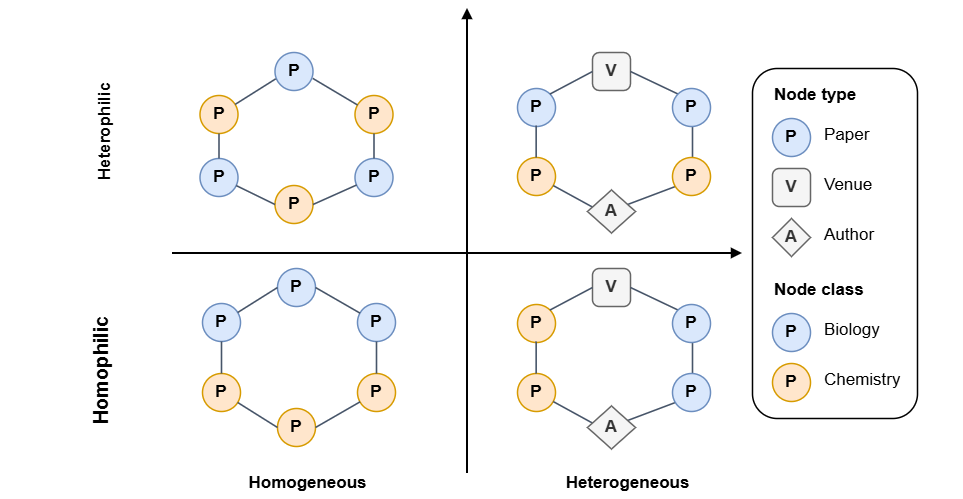
\includegraphics[width=\columnwidth]{figure/Het_HomGraph.drawio.png}
  \caption{An example of heterogeneous heterophilic graph. The graph contains multiple types of nodes and edges, and connected nodes may have different properties.}
  \label{fig:het_hom_graph}
\end{figure}

Many existing methods address either heterogeneous graphs without explicitly considering heterophily \cite{hu2020heterogeneous,mao2023hinormer,he2024spectral,yang2023simple,wang2019heterogeneous,zhang2019heterogeneous} or heterophilic graphs without modeling heterogeneous node and edge types \cite{grover2025spectro,yue2025graph,bodnar2022neural,ribeiro2026cooperative}. Recent methods have begun to address heterogeneous heterophilic graphs through meta-path-based latent subgraphs \cite{lu2026addressing,chen2025adaptive,li2025hetero2net,guo2023homophily,shen2025heterophily,wang2025homophily}, graph rewiring \cite{tao2025cross}, graph transformers \cite{lin2025heterophily}, and sheaf-based mappings \cite{braithwaite2024heterogeneous}. Among these directions, meta-paths can express information that is not contained in either endpoint alone \cite{sun2011pathsim}. For instance, an \texttt{Author-Paper-Author} meta-path describes a co-authorship relation in citation networks, as shown in Figure~\ref{fig:meta_path}. However, existing methods either ignore meta-paths completely, use meta-paths as semantic views, filtered edge sets, or aggregation channels rather than retaining each concrete path instance as part of the propagation structure. For example, an \texttt{A-P-A} meta-path can connect two authors through a shared paper, but after it is converted into an author-author view, the shared paper and the two authorship edges no longer directly shape the propagation operator. This is limiting under heterophily, because whether information should be reinforced or contrasted can depend on the relations along the path, not only on the endpoint connection. This can weaken locality and higher-order information from meta-paths as a part of graph structure.

\begin{figure}
  \centering
  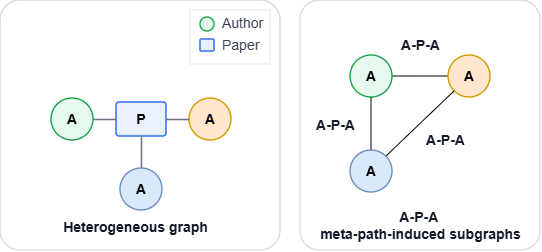
\includegraphics[width=\columnwidth]{figure/meta_path.drawio.png}
  \caption{Illustration of meta-path-induced graph transformation. Under the A-P-A meta-path, authors that share a paper in the original heterogeneous graph are connected in an author-level subgraph.}
  \label{fig:meta_path}
\end{figure}

Manual meta-path specification creates a second bottleneck. Hand-crafted meta-paths are difficult in complex networks, and some useful paths might be ignored \cite{zhong2022pmhgnn,li2024lmsps}. Moreover, datasets often lack such predefined meta-paths. There exists multiple methods for finding useful meta-paths automatically, but they are usually computationally expensive. Some
methods reduce this burden through progressive sampling \cite{li2024lmsps}, searching algorithm \cite{zhang2026mctshgnn,li2023pmmm,li2026amphgnas,sun2025hgsearch}, or reinforcement learning
\cite{zhong2022pmhgnn}.
Although automatic meta-path search reduces reliance on expert knowledge, most methods still select or weight meta-paths at the schema level. However, it is too coarse: a \texttt{PAP} schema may be useful overall, while some concrete \texttt{PAP} instances connect unrelated papers and introduce noise. Schema-level selection must therefore keep noisy instances with useful ones or discard the entire schema. In addition, many search methods select schemas before training the prediction model, so schema choice and instance relevance cannot be refined jointly by the task objective.

To address these challenges, we propose the Heterophilic Heterogeneous Sheaf Neural Network (\method{}), a sheaf–Hodge neural architecture for heterogeneous graphs with heterophily. \method{} represents meta-path instances as higher-order structures by modeling the input graph as a two-dimensional cellular complex. It then learns structural information through sheaf restriction maps and diffusion while preserving the local interactions that give rise to heterophily and heterogeneity.

We further introduce Automatic Meta-Path Selection for Sheaf Neural Networks (\ampss{}), a two-stage component that identifies informative meta-paths during training. \ampss{} learns weights at both the meta-path-schema level and the individual path-instance level.

For graph classification, node and edge sheaf states must be aggregated into a single graph-level representation. Because these states belong to local vector spaces, the readout should be independent of arbitrary choices of local basis. We therefore propose Sheaf Covariance Pooling (\sheafcovpool{}), a gauge- and permutation-invariant readout that aggregates attention-weighted mean and covariance statistics derived from Gram descriptors of node and edge sheaf states. By construction, the resulting graph representation is invariant under the orthogonal transformations associated with \method{}'s restriction maps.

Together, these components form a unified framework for learning meta-paths as higher-order relation in original graphs, heterogeneous, and heterophilic graph representations.




Our main contributions are summarized as follows:
\begin{enumerate}
  \item We introduce \method{}, a heterogeneous sheaf-Hodge framework that retains concrete typed
  path instances as a face-like component on our proposed 2D-cellular graphs, resulting in a learned graph structure that preserves locality without breaking heterophily on heterogeneous graphs.
  \item We propose \ampss{}, a two-stage schema-to-cell selection mechanism that combines
  training-only candidate preselection with differentiable schema- and instance-level refinement
  inside the upper edge Laplacian. This subcomponent allows \method{} to learn which concrete occurrences
  of a schema are useful for the task.
  \item For graph classification, we introduce \sheafcovpool{} as a readout function for graph classification task in \method{}, a gauge-invariant and permutation invariant readout that scores per-node and per-edge learned attention and pools their
  attention-weighted mean and covariance, producing a graph-level representation that is suitable for sheaf neural network.
\end{enumerate}

To this end, we evaluate the framework across node classification, graph classification, and
heterogeneous link prediction. As a result, \method{} achieves the best overall performance across all tasks including node classification, graph classification, and heterogeneous link prediction.

\section{Preliminaries}
\label{sec:background}


\subsection{Heterogeneous graphs}

A heterogeneous graph is a tuple $G=(V,E,\phi,\psi)$, where $V$ and $E$ are the node and edge
sets, $\phi:V\rightarrow\mathcal{T}$ assigns each node a type, and
$\psi:E\rightarrow\mathcal{R}$ assigns each edge a relation type. The realized type sets are
$\mathcal{T}=\{\phi(v):v\in V\}$ and $\mathcal{R}=\{\psi(e):e\in E\}$. The graph is heterogeneous
when it contains more than one node type or more than one relation type, i.e.,
$|\mathcal{T}|>1$ or $|\mathcal{R}|>1$; it reduces to a homogeneous graph when
$|\mathcal{T}|=|\mathcal{R}|=1$ \cite{lu2026addressing}.

\subsection{Homophily and Heterophily}
Homophily describes the tendency of connected nodes to share the same label. For a graph
$G'=(V',E')$ whose endpoint labels are comparable, its edge homophily is
\begin{equation}
  H_{\mathrm{edge}}(G')
  = \frac{1}{|E'|}\sum_{(u,v)\in E'}\mathbf{1}[y_u=y_v],
  \label{eq:background-edge-homophily}
\end{equation}
where $y_u$ is the label of node $u$ and $\mathbf{1}[\cdot]$ is the indicator function
\cite{zhu2020beyond}. Heterophily describes the opposite tendency: adjacent nodes are more likely to have different labels. Larger homophily values indicate stronger label agreement. For heterogeneous graphs, we compute homophily on each meta-path-induced homogeneous subgraph and average across the considered meta-paths \cite{shen2025UHGRL}:
\begin{equation}
    \mathcal{H}
    =
    \frac{1}{|\mathcal{P}|}
    \sum_{p \in \mathcal{P}}
    H_{\mathrm{edge}}(G'_p),
    \label{eq:overall-homophily}
\end{equation}
where $\mathcal{P}$ denotes the set of all considered meta-paths and $G'_p$ is the homogeneous subgraph induced by meta-path $p$.

\subsection{Meta-path}
A meta-path schema of length $\ell$ is a typed relation sequence
\begin{equation}
  \sigma:
  t_0 \xrightarrow{r_1} t_1 \xrightarrow{r_2}\cdots
  \xrightarrow{r_\ell} t_\ell,
  \qquad t_i\in\mathcal{T},\; r_i\in\mathcal{R},
  \label{eq:background-metapath-schema}
\end{equation}
which specifies a composite relation between its endpoint types \cite{sun2011pathsim}. For each
relation $r$, let $A_r\in\{0,1\}^{|V|\times|V|}$ be its adjacency matrix, with
$(A_r)_{uv}=1$ when an edge of type $r$ connects $u$ to $v$. The schema induces the walk-count
matrix
\begin{equation}
  A_\sigma=A_{r_1}A_{r_2}\cdots A_{r_\ell},
  \label{eq:background-metapath-adjacency}
\end{equation}
where $(A_\sigma)_{uv}$ counts the concrete walks from $u$ to $v$ that follow $\sigma$. When
$t_0=t_\ell$, thresholding $A_\sigma$ produces a homogeneous endpoint graph on which
Eq.~\eqref{eq:background-edge-homophily} can be evaluated. For example, the
paper-author-paper schema has $A_{\mathrm{PAP}}=A_{\mathrm{PA}}A_{\mathrm{AP}}$ and connects
papers that share an author. A concrete path instance is an ordered sequence
$f=(v_0,e_1,v_1,\ldots,e_\ell,v_\ell)$ satisfying $\phi(v_i)=t_i$ and $\psi(e_i)=r_i$. Thus,
$\sigma$ describes a type-level pattern, whereas $f$ identifies one occurrence of that pattern in
the observed graph.

\subsection{Cellular sheaves and neural diffusion}

A cellular complex represents a structure using cells of different dimensions. Nodes are
\(0\)-cells, edges are \(1\)-cells, and surfaces bounded by edges are \(2\)-cells. A graph is
therefore a one-dimensional cellular complex, while adding faces produces a two-dimensional
complex. We write \(\sigma\unlhd\tau\) when a lower-dimensional cell \(\sigma\) is incident to a
higher-dimensional cell \(\tau\).

A cellular sheaf \(\cF\) equips this combinatorial structure with local vector spaces and maps
between them. It assigns a vector space, called a \emph{stalk}, \(\cF(\sigma)\) to each cell
\(\sigma\), together with a linear restriction map
\(F_{\sigma\unlhd\tau}:\cF(\sigma)\rightarrow\cF(\tau)\) for every incident pair. These maps
specify how information stored on different cells is transported into a common space.

On a graph \(G=(V,E)\), a cellular sheaf assigns stalks \(\cF(v)\) to nodes and \(\cF(e)\) to
edges. Node and edge assignments form the cochain spaces
\begin{equation}
  C^0(G,\cF)=\bigoplus_{v\in V}\cF(v),
  \qquad
  C^1(G,\cF)=\bigoplus_{e\in E}\cF(e).
\end{equation}
For each incident pair \(v\unlhd e\), a restriction map
\(F_{v\unlhd e}:\cF(v)\rightarrow\cF(e)\) transports the node representation into the shared edge
space. Given an oriented edge \(e=(u\rightarrow v)\), the first coboundary operator
\(\delta_0:C^0(G,\cF)\rightarrow C^1(G,\cF)\) measures disagreement between the transported endpoint
representations:
\begin{equation}
  (\delta_0x)_e
  =
  F_{v\unlhd e}x_v-F_{u\unlhd e}x_u.
  \label{eq:prelim-delta0}
\end{equation}
The corresponding sheaf Laplacian is
\(L_0=\delta_0^{\transpose}\delta_0\), with energy
\(x^{\transpose}L_0x=\lVert\delta_0x\rVert_2^2\). When all stalks are one-dimensional and all
restriction maps are identities, \(L_0\) reduces to the ordinary graph Laplacian.

There are several approaches to sheaf neural networks. Neural Sheaf Diffusion learns restriction maps from node features and uses the resulting Laplacian to propagate information \cite{bodnar2022neural}. This allows connected nodes to be transformed
before comparison, which is useful when their raw features are dissimilar. HetSheaf extends this
mechanism to heterogeneous graphs by conditioning restriction maps on node and relation types
\cite{braithwaite2024heterogeneous}. However, these models define sheaf structure only over observed
node-edge incidences. In contrast, \method{} additionally retains selected meta-path instances as
face-like supports and learns edge-to-face maps, enabling diffusion over an explicit edge cochain.

\section{Methodology}
\label{sec:method}

\subsection{Problem Formulation}

We study supervised learning on directed heterogeneous heterophilic graphs.  The
input is a graph
\(G=(V,E,\phi,\psi,X^{\mathrm{raw}})\), where
\(\phi:V\rightarrow\mathcal{T}\) assigns node types,
\(\psi:E\rightarrow\mathcal{R}\) assigns relation types, and
\(X^{\mathrm{raw}}=\{x_v^{\mathrm{raw}}\}_{v\in V}\) contains type-dependent node features with
\(x_v^{\mathrm{raw}}\in\R^{d_{\phi(v)}}\).  Because different node types may have different feature
spaces, and because adjacent or path-connected nodes may have different labels or dissimilar
attributes, the learner cannot rely on a shared feature encoder or a homophilic aggregation rule.

In addition to the typed graph, the model is given a pool of meta-path schemas
\(\Sigma\), either supplied manually or selected by \ampss{}.  A schema
\(\sigma=(t_0,r_1,t_1,\ldots,r_\ell,t_\ell)\) specifies a valid typed relation sequence, while
\(f=(v_0,e_1,v_1,\ldots,e_\ell,v_\ell)\) denotes one concrete path instance satisfying
\(\phi(v_i)=t_i\) and \(\psi(e_i)=r_i\).  Let \(\mathcal{I}_\sigma\) be the set of observed
instances of schema \(\sigma\), and let
\(\mathcal{I}_\Sigma=\bigcup_{\sigma\in\Sigma}\mathcal{I}_\sigma\).  Unlike methods that collapse a
meta-path into an endpoint-level homogeneous graph, we retain each
\(f\in\mathcal{I}_\Sigma\) as an ordered face-like support over its path edges.

The learning problem is to construct a predictor
\[
  \hat{y}_s
  =
  g_\theta(s;G,\mathcal{I}_\Sigma),
\]
for a task-specific supervised object \(s\).  For node classification, \(s\) is a target node; for
link prediction, \(s\) is a candidate typed node pair; and for graph classification, \(s\) is an
entire graph.  Given labeled training objects \(\mathcal{S}_{\mathrm{train}}\), the parameters are
learned by minimizing
\[
  \min_\theta
  \frac{1}{|\mathcal{S}_{\mathrm{train}}|}
  \sum_{s\in\mathcal{S}_{\mathrm{train}}}
  \mathcal{L}\!\left(g_\theta(s;G,\mathcal{I}_\Sigma),y_s\right).
\]
Thus, the central challenge is to learn type-aware and relation-aware propagation operators that
can use selected meta-path instances as higher-order structure, while avoiding the assumption that
connected nodes should become similar.

\subsection{Framework Overview}

We introduce \method{}, a Heterophilic Heterogeneous Sheaf--Hodge Neural Network for supervised learning on heterogeneous heterophilic graphs. As illustrated in Figure~\ref{fig}, the \method{} framework comprises four stages. First, the \emph{Data Input} stage prepares typed node features, relations, and training-only diagnostic statistics. Second, \method{} employs its Automatic Meta-Path Selection subcomponent, \ampss{}, to construct a compact pool of meta-path schemas and learn the importance of their corresponding path instances. Third, the selected paths are incorporated into the sheaf--Hodge encoder, which learns node--edge--face geometry through restriction maps and performs diffusion over node and edge cochains. Finally, \method{} applies a task-specific prediction head. Node classification reads the final states of selected target nodes, link prediction scores pairs of final node representations, and graph classification uses the \sheafcovpool{} subcomponent to aggregate node and edge sheaf states into a graph-level representation.

Thus, \ampss{} serves as the meta-path selection mechanism within \method{}, while \sheafcovpool{} serves as its graph-level readout for graph classification. All tasks share the same underlying sheaf--Hodge encoder and learned geometric operators.

\begin{figure*}[t]
  \centering
  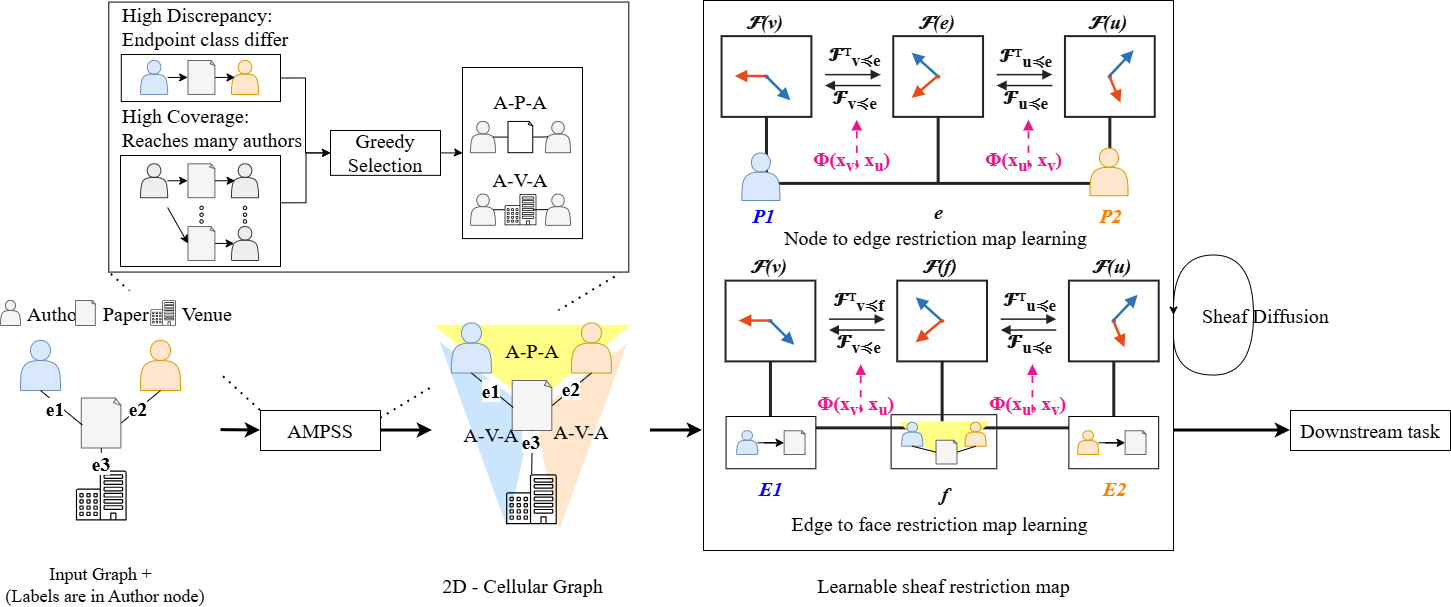
\includegraphics[width=\textwidth]{figure/h2snn_framework_overview.png}
  \caption{Overview of \method{}.  Typed graph data enter a training-only \ampss{} selection stage;
  selected schemas and weighted path instances then parameterize the node-edge-face geometry.
  Node and edge cochains diffuse in parallel before task-specific node, link, or graph prediction,
  with graph classification routed through \sheafcovpool{}.}
  \Description{A left-to-right four-stage diagram.  Data Input feeds AMPSS schema and instance
  selection, which feeds H2S-NN sheaf-Hodge geometry and parallel node and edge diffusion.  The
  output branches to node classification, link prediction, and graph classification through
  SheafCovPool.}
  \label{fig:pipeline}
\end{figure*}



\subsection{Node Stalks and Sheaf Restrictions Initialization}

Firstly, \method{} maps all node types into a shared stalk space and learns relation-aware restrictions
for each typed edge. This is needed because heterogeneous features are not directly comparable since each embedding has a different semantic spaces, and heterophilic edges should measure transported disagreement rather than raw similarity. These
restrictions define the first coboundary \(\delta_0\), which provides the node-to-edge geometry used
by the later edge-to-face construction in cellular sheaves of our \method{}. We therefore map
each type into the common stalk space before comparing adjacent nodes:
\begin{equation}
  h_v^{(0)}
  =\operatorname{Dropout}\!\left[
    \operatorname{GELU}\!\left(
      \operatorname{LN}(W_{\phi(v)}x_v+b_{\phi(v)})+q_{\phi(v)}
    \right)
  \right]\in\R^d ,
  \label{eq:node-encoder}
\end{equation}
where \(W_t,b_t\) are type-specific parameters and \(q_t\) is a learned type embedding.  A learned
node table supplies \(h_v^{(0)}\) when raw attributes are unavailable.  We initialize the diffused
node cochain as \(x^{(0)}=h^{(0)}\), and represent each relation \(r\) by
\(z_r\in\R^{d_r}\).

To ensure Relation-conditioned restrictions, given an oriented edge \(e=(u\xrightarrow{r}v)\), two relation-conditioned networks infer
\(F_{u\unlhd e},F_{v\unlhd e}\in\R^{d\times d}\) from
\(h_u^{(0)}\), \(h_v^{(0)}\), and \(z_r\).  Each restriction is scaled orthogonal:
\begin{equation}
  F_{v\unlhd e}=\lambda_{v,e}Q_{v,e},
  \qquad Q_{v,e}^{\transpose}Q_{v,e}=I,
  \qquad \lambda_{v,e}>0 ,
  \label{eq:conformal-map}
\end{equation}
and analogously for \(F_{u\unlhd e}\).  The orthogonal factor aligns local coordinates, while the
positive scale adjusts the strength of the incidence.  These restrictions define the first
coboundary immediately:
\begin{equation}
  (\delta_0x)_e
  =F_{v\unlhd e}x_v-F_{u\unlhd e}x_u .
  \label{eq:delta0}
\end{equation}
Thus, \(\delta_0x\) measures endpoint disagreement after relation-specific transport rather than
raw feature difference. Then, we initialize the edge cochain with a learnable MLP,
\begin{equation}
  s_e^{(0)}
  =\operatorname{MLP}_{\mathrm{init}}\!\left(
    h_u^{(0)}\concat h_v^{(0)}\concat z_r
    \concat(\delta_0h^{(0)})_e
  \right),
  \label{eq:edge-init}
\end{equation}
so \(s^{(0)}\neq\delta_0h^{(0)}\) in general.  This preserves an edge component outside
\(\operatorname{im}\delta_0\) for the subsequent lower- and upper-Hodge interactions.

\subsection{\ampss{}: Adaptive Meta-Path Schema-to-Cell Selection}
\label{sec:ampss}

\ampss{} separates economical structure search from task-driven refinement.  The first stage is a
non-differentiable, training-only construction of a candidate pool; the second stage learns soft
weights for the retained schemas and their concrete instances jointly with \method{}.

\paragraph{Stage I: candidate generation and preselection.}
The first stage constructs a small set of typed higher-order supports before the neural model is
trained.  It does so at the level of the heterogeneous schema rather than by immediately traversing
all concrete node paths.  We first form a directed type graph whose nodes are entity types and whose
directed edges are relation types, e.g., \(P\xrightarrow{\mathrm{writes}^{-1}}A\) and
\(A\xrightarrow{\mathrm{writes}}P\) in a paper--author network.  A bounded depth-first search over
this type graph enumerates valid schema candidates
\(\sigma=(t_0,r_1,t_1,\ldots,r_\ell,t_\ell)\) subject to the allowed length range and, when
required by the task, the start and end target types.  This step therefore proposes only type-valid
relational routes; it does not yet decide that any route is useful.

For each candidate schema, \ampss{} then samples concrete instances in the original graph.  Starting
from nodes of type \(t_0\), it follows the prescribed relation sequence
\((r_1,\ldots,r_\ell)\) and records paths
\(f=(v_0,e_1,v_1,\ldots,e_\ell,v_\ell)\) whose node and edge types match the schema.  Separate
budgets cap the number of candidate schemas, the number of instances expanded from one anchor node,
the number of instances retained for one schema, and the total number of materialized instances.
These caps make the construction economical while still exposing the model to the main typed
relational patterns present in the graph.

The preselection score is designed to keep schemas that are both informative and usable as
face-like supports.  For node classification, training labels are propagated for a fixed number of
steps to obtain soft endpoint distributions \(\widehat y_v\).  A concrete path receives a large
discrepancy when its two endpoints carry different training-derived class evidence, and a schema
receives the average discrepancy of its sampled instances:
\begin{equation}
  d(f)=\norm{\widehat y_{v_0}-\widehat y_{v_\ell}}_2^2,
  \qquad
  D(\sigma)=\frac{1}{|\mathcal{I}_{\sigma}|}
  \sum_{f\in\mathcal{I}_{\sigma}}d(f).
  \label{eq:discrepancy}
\end{equation}
Intuitively, this favors schemas whose endpoints expose nontrivial class contrast under the
training signal, which can create useful edge-level disagreement for the subsequent Hodge diffusion.
For link prediction, the same idea is implemented with two propagated endpoint-role channels that
mark source and target positions using training-positive edges only.  Neither validation nor test
labels or links contribute to these statistics.

For graph classification, endpoint discrepancy is not the relevant signal.  Let
\(n_{\sigma,c}^{\mathrm{pres}}\) be the number of training graphs of class \(c\) in which schema
\(\sigma\) occurs, \(N_c\) the number of training graphs in that class, and \(n_\sigma\) the total
number of its materialized instances.  The presence score is
\begin{equation}
  P_G(\sigma)
  =\operatorname{Var}_{c}\!\left(
    \frac{n_{\sigma,c}^{\mathrm{pres}}}{\max(N_c,1)}
  \right)+10^{-3}\log(1+n_\sigma).
  \label{eq:graph-presence-score}
\end{equation}
This favors schemas whose presence differs across training classes, with frequency used only as a
small tie breaker.

For node and link tasks, \ampss{} greedily builds the selected pool one schema at a time.  The
score combines four quantities.  The discrepancy \(D(\sigma)\) measures task relevance.  The
endpoint coverage \(C(\sigma)\) measures how many target-type endpoints are reached by the sampled
instances, so a schema that appears only in a tiny corner of the graph is not selected merely
because it has a high local score.  The type diversity \(V(\sigma)\) rewards schemas that pass
through multiple semantic types rather than repeatedly using the same type pattern.  Finally,
\(J(\sigma,\sigma')\) measures endpoint-set overlap with an already selected schema
\(\sigma'\), discouraging several selected schemas from describing nearly the same region of the
graph.  Given the current pool \(S\), the greedy score is
\begin{equation}
  q(\sigma\mid S)=
  \frac{D(\sigma)^{a_d}C(\sigma)^{a_c}V(\sigma)^{a_v}}
       {1+\max_{\sigma'\in S}J(\sigma,\sigma')} ,
  \label{eq:topology-score}
\end{equation}
The numerator prefers schemas that are informative, sufficiently covered, and semantically varied;
the denominator lowers the priority of schemas that are redundant with the pool already chosen.
Graph tasks use the class-presence score \(P_G(\sigma)\) instead of Equation~\ref{eq:topology-score}.
After this greedy pass, the selected schemas are materialized as ordered path supports, together
with the closure pairs used by the node-side correction.  This entire stage fixes the candidate
support and is intentionally non-differentiable; the next stage decides how strongly the retained
schemas and their individual instances should participate in the learned operator.

\paragraph{Stage II: differentiable schema and instance refinement.}
Preselection decides what can be considered; it does not force every retained structure to
contribute equally.  We learn one gate per schema and a state-dependent gate for every path
instance:
\begin{equation}
  \begin{aligned}
  \alpha_\sigma&=\operatorname{sigmoid}(\theta_\sigma),\\
  \beta_f&=\operatorname{sigmoid}\!\left(
    g_\beta(h_{v_0}^{(0)}\concat h_{v_\ell}^{(0)}\concat e_\sigma)
  \right),\\
  w_f&=\alpha_{\sigma(f)}\beta_f .
  \end{aligned}
  \label{eq:gates}
\end{equation}
Here \(e_\sigma\) is a learned schema embedding.  Schema logits are warm-started from standardized
preselection scores, while \(\beta_f\) lets two instances of the same schema have different
effects.  During training, partial-schema propagation retains each schema with probability
\(p_{\mathrm{keep}}\) and rescales a retained gate by \(1/p_{\mathrm{keep}}\), following the
stabilization idea of partial message propagation \cite{li2023pmmm}.

The discovery loss applies complementary pressures rather than a single hard selection rule:
\begin{equation}
  \begin{aligned}
  \cL_{\mathrm{disc}}={}&
  \lambda_s\cL_{\mathrm{sparse\text{-}schema}}
  +\lambda_i\cL_{\mathrm{sparse\text{-}instance}}
  +\lambda_r\cL_{\mathrm{redundancy}}\\
  &+\lambda_v\cL_{\mathrm{coverage}}
  +\lambda_{\mathrm{cost}}\cL_{\mathrm{cost}}
  +\lambda_H\cL_{\mathrm{entropy}} .
  \end{aligned}
  \label{eq:discovery-loss}
\end{equation}
Schema and instance terms discourage diffuse activation; redundancy penalizes similar active
coverage profiles; the negative coverage reward discourages a trivial empty pool; cost suppresses
long, frequently instantiated schemas; and entropy minimization sharpens schema decisions.  These
terms refine only the preselected pool and do not make candidate generation differentiable.

\begin{algorithm}[t]
  \caption{\ampss{} candidate preselection and differentiable refinement}
  \label{alg:ampss}
  \begin{algorithmic}[1]
    \REQUIRE Typed relation graph, training split, schema and instance budgets
    \STATE \textbf{Stage I: Candidate generation and training-only preselection}
    \STATE Enumerate bounded typed schemas and sample concrete instances
    \STATE Compute node/link discrepancy scores or graph presence scores
    \STATE Greedily retain a compact pool \(\Sigma\) and materialize its path supports
    \STATE Initialize \(\theta_\sigma\) from standardized preselection scores
    \FOR{each training epoch}
      \STATE \textbf{Stage II: Differentiable schema and instance refinement}
      \STATE Use uniform face weights during warm-up
      \STATE Compute \(\alpha_\sigma\), \(\beta_f\), and \(w_f=\alpha_{\sigma(f)}\beta_f\)
      \STATE Apply partial-schema propagation with keep probability \(p_{\mathrm{keep}}\)
      \STATE Run matrix-free sheaf-Hodge diffusion and the task readout
      \STATE Optimize Equation~\ref{eq:loss}
    \ENDFOR
  \end{algorithmic}
\end{algorithm}

\subsection{2D-cellular Sheaf-Hodge Geometry Construction}

The sheaf-Hodge encoder begins by defining the cellular object on which diffusion is performed.
A graph is already a \(1\)-dimensional cellular complex: nodes are \(0\)-cells and typed edges are
\(1\)-cells.  \method{} extends this complex with selected meta-path instances.  A concrete
instance
\[
  f=(v_0,e_1,v_1,\ldots,e_\ell,v_\ell)
\]
is treated as a face-like \(2\)-cell supported on its ordered path edges.  Since an open path is not
itself the boundary of a \(2\)-cell, the model also attaches one closure \(1\)-cell
\(e_{\mathrm{cl}}=(v_\ell\rightarrow v_0)\).  Thus the boundary used by the upper Hodge term is
\[
  \partial f=(e_1,\ldots,e_\ell,e_{\mathrm{cl}}).
\]
This keeps the intermediate nodes and relations visible to the operator, rather than replacing the
meta-path by a shortcut edge between \(v_0\) and \(v_\ell\).

We write \(\sigma\unlhd\tau\) when a lower-dimensional cell \(\sigma\) is incident to a
higher-dimensional cell \(\tau\).  A cellular sheaf \(\cF\) equips each cell with a local vector
space, or \emph{stalk}, and assigns a linear restriction map
\(F_{\sigma\unlhd\tau}:\cF(\sigma)\rightarrow\cF(\tau)\) to every incidence.  In \method{}, node,
edge, and face stalks all have dimension \(d\).  The node cochain space and the extended edge
cochain space are
\begin{equation}
  C^0(\cF)=\bigoplus_{v\in V}\cF(v),
  \qquad
  C^1(\cF)=\bigoplus_{e\in E\cup E_{\mathrm{cl}}}\cF(e),
\end{equation}
where \(E_{\mathrm{cl}}\) denotes the closure \(1\)-cells introduced by the selected path
instances.  The selected instances form the face cochain space
\begin{equation}
  C^2(\cF)=\bigoplus_{f\in\mathcal{I}_{\Sigma}}\cF(f).
\end{equation}

The node-to-edge restrictions from the previous subsection define the first coboundary
\(\delta_0:C^0(\cF)\rightarrow C^1(\cF)\).  For an oriented edge \(e=(u\rightarrow v)\),
\begin{equation}
  (\delta_0x)_e
  =
  F_{v\unlhd e}x_v-F_{u\unlhd e}x_u .
  \label{eq:background-delta0}
\end{equation}
Thus \(\delta_0x\) is not a homophilic average.  It is a transported endpoint disagreement, which
is the edge-level signal used by the later Hodge operator.  The next step is to define compatible
edge-to-face restrictions, so that selected path supports can act on edge states without breaking
the cochain structure.

\subsection{Path-Supported Edge-Face Geometry}
\label{sec:face-geometry}

The edge-face construction turns each selected path instance into a face-like operator on edge
cochains.  For a selected \(P\!-\!A\!-\!P\) instance, the two path edges remain two boundary edges
of one support; the instance is not collapsed into a paper-paper shortcut.  For a general instance
\(f=(v_0,e_1,v_1,\ldots,e_\ell,v_\ell)\), \method{} first learns a single free map \(A_f\) from the
ordered path.  This map fixes the face stalk's frame for that instance.  The individual
edge-to-face maps are then derived from \(A_f\) and the node-to-edge restrictions already used by
\(\delta_0\).

Every face group materializes one schema, so all instances in the group have the same length
\(\ell\) and the same relation sequence \((r_1,\ldots,r_\ell)\).  What varies across instances is
the ordered tuple of node states.  The default face encoder therefore concatenates the node states
in path order together with the schema's relation embeddings and applies one network per length:
\begin{equation}
  A_f
  =\operatorname{reshape}\!\Big(
    \operatorname{MLP}_{\ell}\big(
      h_{v_0}^{(0)}\concat\cdots\concat h_{v_\ell}^{(0)}
      \concat z_{r_1}\concat\cdots\concat z_{r_\ell}
    \big),\,d,d\Big).
  \label{eq:face-map}
\end{equation}
Position is preserved because each slot of the concatenation has its own parameters.  Therefore
\(A_f\) can distinguish \((v_0,\ldots,v_\ell)\) from a reordered tuple.  Since
\(\operatorname{MLP}_\ell\) is shared across schemas of the same length, the parameter count depends
on the set of path lengths rather than on the number of selected schemas.

The per-edge maps are not emitted independently.  The upper Hodge term should measure edge-level
curl around a selected path support, not create curl from a pure node-induced gradient.  Therefore
the edge-to-face maps must compose with the node-to-edge maps beneath them.  \method{} enforces this
by carrying a transport to the base vertex \(v_0\) along the path:
\begin{equation}
  \begin{aligned}
  T_{v_0}&=A_f,
  \qquad
  T_{v_i}=T_{v_{i-1}}F_{u\unlhd e_i}^{-1}F_{v\unlhd e_i},\\
  F_{e_i\unlhd f}&=T_{v_{i-1}}F_{u\unlhd e_i}^{-1},
  \end{aligned}
  \label{eq:transport}
\end{equation}
where \(u=v_{i-1}\) and \(v=v_i\) are the endpoints of \(e_i\).  The inverse is available in closed
form: by Eq.~\eqref{eq:conformal-map}, each node-to-edge map is a positive scale times an
orthogonal factor, so \(F^{-1}=F^{\transpose}/\lambda^2\).  No general linear solve is required.

The closure edge is also defined from the same transport:
\begin{equation}
  F_{v_0\unlhd e_{\mathrm{cl}}}=I,
  \qquad
  F_{v_\ell\unlhd e_{\mathrm{cl}}}=T_{v_0}^{-1}T_{v_\ell},
  \qquad
  F_{e_{\mathrm{cl}}\unlhd f}=A_f .
  \label{eq:closure-maps}
\end{equation}
The middle map is the path holonomy
\(\prod_i F_{u\unlhd e_i}^{-1}F_{v\unlhd e_i}\), so the closure edge adds no learned relation
parameters.  It is a bookkeeping \(1\)-cell that makes ``walk along the path and return'' a closed
boundary cycle, not an assertion that the endpoints have an observed relation.

Let \(\eta(e,f)\in\{-1,+1\}\) be the stored incidence orientation.  The schema-instance gate enters
the weighted second coboundary:
\begin{equation}
  (\delta_{1,w}s)_f
  =\sqrt{w_f}\sum_{e\in\partial f}
    \eta(e,f)F_{e\unlhd f}s_e .
  \label{eq:delta1}
\end{equation}
Writing
\(B_fs=\sum_{e\in\partial f}\eta(e,f)F_{e\unlhd f}s_e\), its upper-Hodge contribution is
\begin{equation}
  \delta_{1,w}^{\transpose}\delta_{1,w}
  =\sum_{\sigma\in\Sigma}\sum_{f\in\mathcal{I}_{\sigma}}
    w_f B_f^{\transpose}B_f .
  \label{eq:weighted-up}
\end{equation}
The square root makes each face contribute linearly in \(w_f\), not quadratically.
Figure~\ref{fig:sheaf-hodge-operator} makes this boundary explicit.

\begin{proposition}[Exact cochain condition]
\label{prop:chain}
For every instance whose node sequence is a simple path, the maps of
Eqs.~\eqref{eq:transport}--\eqref{eq:closure-maps} satisfy
\(\delta_{1,w}\delta_0=0\) identically, for every node cochain and every value of the learned
parameters, with no assumption that the sheaf has trivial holonomy.
\end{proposition}

\begin{proof}
By construction \(F_{e_i\unlhd f}F_{u\unlhd e_i}=T_{v_{i-1}}\) and
\(F_{e_i\unlhd f}F_{v\unlhd e_i}=T_{v_i}\), so the \(i\)-th boundary term of
\(\delta_{1,w}\delta_0x\) equals
\(T_{v_i}x_{v_i}-T_{v_{i-1}}x_{v_{i-1}}\).  Summing over the path telescopes to
\(T_{v_\ell}x_{v_\ell}-T_{v_0}x_{v_0}\).  Eq.~\eqref{eq:closure-maps} gives
\(F_{e_{\mathrm{cl}}\unlhd f}F_{v_0\unlhd e_{\mathrm{cl}}}=T_{v_0}\) and
\(F_{e_{\mathrm{cl}}\unlhd f}F_{v_\ell\unlhd e_{\mathrm{cl}}}=T_{v_\ell}\), so the closure term
contributes \(T_{v_0}x_{v_0}-T_{v_\ell}x_{v_\ell}\) and the total vanishes.  Simplicity is required
because the transport assigns one map per node position; a revisited node, including a coincident
endpoint pair, would be assigned two values.
\end{proof}

\noindent This condition explains why the face maps are built by transport.  Exact node-induced
edge signals lie in \(\operatorname{im}\delta_0\), and the upper term should not treat them as face
curl.  The implementation tests this condition directly for the supported face encoders and
face-map parameterizations.

\begin{figure}[t]
  \centering
  \fbox{\rule{0pt}{4.2cm}\rule{0.94\columnwidth}{0pt}}
  %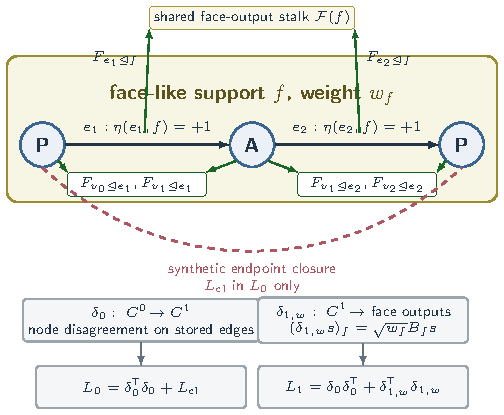
\includegraphics[width=\columnwidth]{figure/h2snn_sheaf_hodge_operator.pdf}
  \caption{AMPSS-selected path instances define a sheaf-Hodge operator. Currently in construction.}
  \label{fig:sheaf-hodge-operator}
\end{figure}

\subsection{Matrix-Free Sheaf-Hodge Diffusion}
\label{sec:closure}

After the node-edge and edge-face maps have been constructed, \method{} diffuses node and edge
cochains with the induced Hodge operators.  The two coboundaries give one node operator and one edge
operator:
\begin{align}
  L_0x
  &=\delta_0^{\transpose}\delta_0x,
  \label{eq:l0}\\
  L_1s
  &=\underbrace{\delta_0\delta_0^{\transpose}s}_{\text{lower edge term}}
    +\underbrace{\delta_{1,w}^{\transpose}\delta_{1,w}s}_{\text{upper edge term}} .
  \label{eq:l1}
\end{align}
The lower edge term compares edge signals through their incident nodes; the upper term couples the
edges of a boundary cycle through their shared face.  Because the closure \(1\)-cell of
Section~\ref{sec:face-geometry} is an ordinary member of the extended edge set, it enters
\(\delta_0\), \(L_0\), and the lower edge term exactly like a data edge; no separate node-side
correction is applied.  Its restriction maps are the path holonomy of Eq.~\eqref{eq:transport}, so
it introduces no parameters of its own.  A positive scale \(\gamma\) can be applied to these closure
restrictions and compensated inside \(F_{e_{\mathrm{cl}}\unlhd f}\), leaving
Proposition~\ref{prop:chain} unaffected while tuning how strongly the boundary cycle closes at the
node level.

Starting from \(x^{(0)}=h^{(0)}\) and the independently initialized edge cochain \(s^{(0)}\),
\(K\) explicit Euler steps give
\begin{equation}
  \begin{aligned}
  x^{(k+1)}&=x^{(k)}-\eta_0L_0x^{(k)},\\
  s^{(k+1)}&=s^{(k)}-\eta_1L_1s^{(k)},
  \qquad k=0,\ldots,K-1 .
  \end{aligned}
  \label{eq:diffusion}
\end{equation}
The positive step sizes may be learned.  Node and edge cochains evolve in parallel under geometry
inferred from the same initial node states; there is no cross-rank recurrence between Euler steps.
Layer normalization yields the terminal states \(x^\star\) and \(s^\star\).

Execution is matrix-free.  The model applies \(\delta_0\), \(\delta_0^{\transpose}\),
\(\delta_{1,w}\), and \(\delta_{1,w}^{\transpose}\) by batching local restriction maps and
aggregating incident contributions, without materializing global \(Nd\times Nd\) or
\(Md\times Md\) matrices.  Three implementation boundaries remain consequential.  First,
\(\delta_{1,w}\) spans the complete boundary cycle: the \(\ell\) path edges together with the
closure \(1\)-cell.  Second, signed incidences are supported, and the uniform \(+1\) used here is
the correct boundary map precisely because enumeration traverses every edge along its stored
direction and stores the closure cell oriented along the cycle; the pipeline asserts this rather
than assuming it.  Third, because faces must be simple paths for the transport of
Eq.~\eqref{eq:transport} to be well defined, instances that revisit a node, including those whose
endpoints coincide, are excluded during enumeration.  Under these constraints,
\(\delta_{1,w}\delta_0=0\) is not encouraged by a penalty but holds identically
(Proposition~\ref{prop:chain}).



\subsection{\sheafcovpool{}}

In sheaf neural diffusion, each node stores its embedding in its own local coordinate system, so embeddings from different nodes cannot simply be pooled together. We therefore introduce \sheafcovpool{}, a readout function that combines node and edge information into a single graph embedding while ignoring these arbitrary coordinate choices. As a result, the graph representation captures the meaningful relationships encoded in \(x^\star\), \(h^{(0)}\), and \(s^\star\), ensuring that the final graph representation reflects the underlying structural information, not the specific basis used to represent each embedding.

The readout first forms small view stacks for nodes and edges.  For a node \(v\), the three views
are its diffused node state, its initial typed state, and the mean state of incident edges.  For an
edge \(e\), the views are the post-diffusion node-to-edge disagreement, the initial disagreement,
and the diffused edge state:
\begin{equation}
  \begin{aligned}
  Z_v^{(0)}
  &=\begin{bmatrix}x_v^\star&h_v^{(0)}&\bar s_v^\star\end{bmatrix}
    \in\R^{d\times3},\\
  Z_e^{(1)}
  &=\begin{bmatrix}
    (\delta_0x^\star)_e&(\delta_0h^{(0)})_e&s_e^\star
  \end{bmatrix}
    \in\R^{d\times3}.
  \end{aligned}
\end{equation}
The Gram descriptor
\[
  G_i^{(r)}=(Z_i^{(r)})^{\transpose}Z_i^{(r)}\in\R^{3\times3},
  \qquad r\in\{0,1\},
\]
records only inner products among these views.  If a local orthogonal gauge changes coordinates as
\(Z_i^{(r)}\mapsto Q_iZ_i^{(r)}\), then \(G_i^{(r)}\) is unchanged.  Thus the classifier sees, for
example, how strongly a node's final state aligns with its initial state or with its incident-edge
summary, but not the arbitrary orientation of the stalk basis.

Nodes and edges play different roles, so separate networks project their descriptors:
\(u_i^{(r)}=\rho_r(\operatorname{vec}G_i^{(r)})\in\R^{d_p}\).  A learned score then selects which
nodes or edges are most informative inside graph \(g\), while the per-graph softmax keeps the
summary permutation invariant:
\begin{equation}
  a_i^{(r)}
  =\frac{\exp(g_r(u_i^{(r)}))}
         {\sum_{j\in\mathcal{C}_r(g)}\exp(g_r(u_j^{(r)}))},
  \qquad
  \mu_r(g)=\sum_{i\in\mathcal{C}_r(g)}a_i^{(r)}u_i^{(r)} .
\end{equation}
Here \(\mathcal{C}_0(g)\) and \(\mathcal{C}_1(g)\) are the nodes and edges of \(g\).  The weighted
mean tells what evidence is present on average, but not whether that evidence is uniform or
concentrated in a few parts of the graph.  \sheafcovpool{} therefore also keeps a weighted
covariance:
\begin{equation}
  \Sigma_r(g)
  =\sum_{i\in\mathcal{C}_r(g)}a_i^{(r)}
    (u_i^{(r)}-\mu_r(g))(u_i^{(r)}-\mu_r(g))^{\transpose}.
\end{equation}
Finally, the graph MLP consumes
\begin{equation}
  \gamma_g=
  \bigl[
  \mu_0(g)\concat\operatorname{triu}(\Sigma_0(g))
  \concat\mu_1(g)\concat\operatorname{triu}(\Sigma_1(g))
  \bigr].
\end{equation}
The result is a single-level readout that uses node and edge evidence, preserves first- and
second-order graph statistics, and remains invariant to node/edge order and orthogonal stalk gauges.

\begin{figure}[t]
  \centering
  \fbox{\rule{0pt}{4.2cm}\rule{0.94\columnwidth}{0pt}}
  %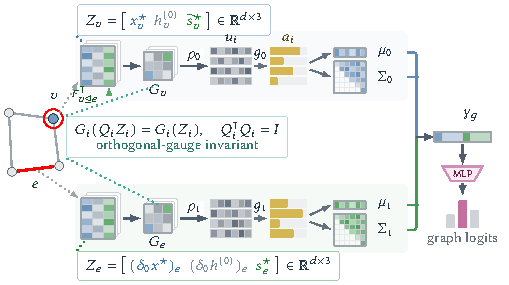
\includegraphics[width=\columnwidth]{figure/sheafcovpool_architecture.pdf}
  \caption{\sheafcovpool{} graph readout. Node and edge view stacks become
  gauge-invariant Gram descriptors; separate attention weights their first and second moments
  before graph classification.}
  \Description{Two parallel node and edge branches.  Each starts with three stalk-valued views,
  forms a Gram descriptor, applies a learned projection and invariant attention, and computes a
  weighted mean and covariance.  Upper-triangular covariance vectors join the means, and the two
  branches concatenate before an MLP outputs graph logits.}
  \label{fig:sheafcovpool}
\end{figure}

\subsection{Training Objective}

\method{} is trained with the supervised task loss and, in auto-discovery mode, the scheduled
\ampss{} discovery objective:
\begin{equation}
  \cL
  =\cL_{\mathrm{task}}
   +\rho(t)\cL_{\mathrm{disc}} .
  \label{eq:loss}
\end{equation}
Here \(\cL_{\mathrm{task}}\) is the task-specific loss, cross-entropy for single-label node and graph classification, and
binary cross-entropy for multi-label classification or link prediction. The \(\cL_{\mathrm{disc}}\) loss combines
the schema- and instance-level gate regularizers used by \ampss{}. The time-dependent coefficient \(\rho(t)\) keeps the discovery regularizers inactive during warm-up and then increases their influence, so the model can first learn task-relevant signals before the \ampss{} discovery process to make the model learn the task first, prevent the discovery process from being collapsed too early.



\section{Experiments}
\label{sec:experiments}


Model selection was performed using hyperparameter sweeps, and the full per-dataset hyperparameters are listed in Appendix~\ref{app:hyperparameters}. To ensure a fair comparison, we ran each experiment with five random seeds and report the mean performance with standard deviation. The code is available at \url{placeholder_for_code_repository.com}. Results for node classification, link prediction, and graph classification are reported in Tables~\ref{tab:node-cls}, \ref{tab:link-pred}, and~\ref{tab:graph-cls}, respectively. Baselines are grouped by graph type and homophily assumption: Hom./hom., Het./hom., Hom./het., and Het./het., where the first term denotes whether the graph is treated as homogeneous or heterogeneous, and the second denotes whether the method targets homophilic or heterophilic settings.

\subsection{Node Classification}
\label{sec:setup-node}


\paragraph{Datasets.}
On the node classification task, we used three benchmark heterogeneous graph datasets: DBLP \cite{lv2021hgb} and IMDB \cite{lv2021hgb}, and ACM \cite{wang2019han}. The statistics of these datasets are summarized in Table~\ref{tab:node-datasets} given in
Appendix~\ref{app:benchmark-datasets}.


\paragraph{Baselines.} We compared \method{} against four groups of baselines: (i) homogeneous homophilic models, including GCN
\cite{kipf2017gcn}, GAT \cite{velickovic2018gat}, and ChebNetII \cite{he2022chebnetii}; (ii) homogeneous heterophilic models, including NSD
\cite{bodnar2022neural} and CSNN \cite{ribeiro2026cooperative}; (iii)
heterogeneous homophilic models, including HAN \cite{wang2019han}, SeHGNN \cite{yang2023sehgnn},
HiNormer \cite{mao2023hinormer}, and PSHGCN \cite{he2024spectral}; and heterogeneous heterophilic models, including HDHGR \cite{guo2023homophily}, Hetero$^2$Net \cite{li2025hetero2net}, H2SGNN
\cite{lu2026addressing}, HetSheaf \cite{braithwaite2024heterogeneous}, and LatGRL
\cite{shen2025heterophily}.


\paragraph{Evaluation Settings.} We followed the HGB benchmark \cite{lv2021hgb} by using the training/validation/test splits in a ratio of 20\%/20\%/60\% on transductive learning. We used Macro-F1 and Micro-F1 as the evaluation metrics.

\paragraph{Results.}
From the results in Table~\ref{tab:node-cls}, \method{} achieved the best performance on all three benchmark datasets in node classification tasks. \method{} outperforms every baselines in every dataset and every setting. This demonstrates the effectiveness of \method{} in capturing complex heterogeneous graph structures and relationships, leading to improved node classification performance.

\begin{table*}[t]
  \centering
  \caption{Performance on node classification benchmarks reporting in Macro-F1 and Micro-F1. Best values are bold.}
  \label{tab:node-cls}
  \scriptsize
  \resizebox{0.8\textwidth}{!}{%
  \begin{tabular}{llcccccc}
    \toprule
    & &
    \multicolumn{2}{c}{DBLP (59.76)} &
    \multicolumn{2}{c}{ACM (72.39)} &
    \multicolumn{2}{c}{IMDB (50.04)} \\
    \cmidrule(lr){3-4}
    \cmidrule(lr){5-6}
    \cmidrule(lr){7-8}
    \textbf{Group} & \textbf{Model}
    & Macro & Micro
    & Macro & Micro
    & Macro & Micro \\
    \midrule

    \multirow{3}{*}{Hom./hom.}
    & GCN
    & $90.77 \pm 0.76$
    & $90.28 \pm 0.20$
    & $91.63 \pm 0.44$
    & $91.38 \pm 0.39$
    & $62.33 \pm 0.58$
    & $67.69 \pm 0.59$ \\

    & GAT
    & $94.39 \pm 1.03$
    & $92.52 \pm 0.27$
    & $92.07 \pm 0.57$
    & $90.71 \pm 0.21$
    & $62.13 \pm 0.26$
    & $68.09 \pm 0.48$ \\
    
    & ChebNetII
    & $92.89 \pm 1.07$
    & $92.67 \pm 0.50$
    & $91.70 \pm 0.27$
    & $91.59 \pm 0.27$
    & $62.97 \pm 0.66$
    & $68.47 \pm 0.55$ \\

    \midrule

    \multirow{2}{*}{Het./hom.}
    & NSD
    & $92.96 \pm 0.21$
    & $93.42 \pm 0.37$
    & $92.33 \pm 0.78$
    & $92.05 \pm 0.69$
    & $61.61 \pm 0.26$
    & $65.23 \pm 0.51$ \\


    & CSNN
    & $93.73 \pm 0.95$
    & $92.12 \pm 0.19$
    & $93.13 \pm 0.94$
    & $92.81 \pm 0.83$
    & $62.92 \pm 0.34$
    & $62.59 \pm 0.22$ \\


    \midrule

    \multirow{4}{*}{Hom./het.}
    & HAN
    & $91.78 \pm 0.92$
    & $92.24 \pm 0.86$
    & $90.88 \pm 0.67$
    & $91.61 \pm 1.07$
    & $61.95 \pm 0.36$
    & $67.76 \pm 0.51$ \\

    & SeHGNN
    & $95.52 \pm 0.98$
    & $95.48 \pm 0.78$
    & $94.38 \pm 1.00$
    & $94.04 \pm 0.73$
    & $72.01 \pm 0.65$
    & $72.59 \pm 0.18$ \\

    & HiNormer
    & $94.06 \pm 0.40$
    & $94.14 \pm 0.46$
    & $91.87 \pm 0.26$
    & $89.64 \pm 0.39$
    & $64.13 \pm 0.19$
    & $67.53 \pm 0.32$ \\

    & PSHGCN
    & $95.58 \pm 0.80$
    & $95.70 \pm 0.54$
    & $93.66 \pm 0.53$
    & $94.70 \pm 0.39$
    & $71.82 \pm 0.34$
    & $74.34 \pm 0.84$ \\
    \midrule

    \multirow{5}{*}{Het./het.}
    & HDHGR
    & $95.35 \pm 0.81$
    & $95.00 \pm 0.77$
    & $93.99 \pm 0.35$
    & $94.13 \pm 0.87$
    & $59.41 \pm 0.22$
    & $59.63 \pm 0.35$ \\

    & Hetero2Net
    & $93.54 \pm 1.11$
    & $93.54 \pm 0.79$
    & $94.05 \pm 0.71$
    & $92.87 \pm 0.82$
    & $65.34 \pm 0.68$
    & $70.63 \pm 0.69$ \\

    & H2SGNN
    & $95.82 \pm 0.41$
    & $95.11 \pm 0.22$
    & $94.90 \pm 0.49$
    & $94.08 \pm 0.44$
    & $74.23 \pm 0.31$
    & $75.29 \pm 0.86$ \\

    & HetSheaf
    & $93.87 \pm 0.00$
    & $93.77 \pm 0.00$
    & $95.09 \pm 0.00$
    & $94.94 \pm 0.00$
    & $64.65 \pm 0.00$
    & $67.18 \pm 0.00$ \\

    & LatGRL
    & $94.32 \pm 0.44$
    & $94.51 \pm 0.42$
    & $93.47 \pm 0.71$
    & $92.29 \pm 0.43$
    & $58.27 \pm 0.46$
    & $58.81 \pm 0.65$ \\
    \midrule

    Ours
    & \textbf{\method{}}
    & $\mathbf{96.01 \pm 0.58}$
    & $\mathbf{96.31 \pm 0.40}$
    & $\mathbf{95.91 \pm 1.15}$
    & $\mathbf{95.72 \pm 0.68}$
    & $\mathbf{75.05 \pm 0.22}$
    & $\mathbf{76.68 \pm 0.19}$ \\
    \bottomrule
  \end{tabular}%
  }
\end{table*}



\subsection{Graph classification}
\label{sec:setup-graph}
\paragraph{Datasets.}
On the graph classification task, we used four benchmark heterogeneous graph datasets from TUDataset \cite{morris2020tudataset}: biological graphs, including PROTEINS and ENZYMES, and chemical compound graphs, including MUTAG and NCI1. To make those graphs heterogeneous, we treated the node and edge labels supplied by TUDataset as different node and edge types. The detail is  in Table~\ref{tab:graph-datasets} given in Appendix~\ref{app:benchmark-datasets}.



\paragraph{Baselines.} We compared \method{} against four groups of baselines: (i) homogeneous homophilic models, including GCN \cite{kipf2017gcn} and GAT \cite{velickovic2018gat}; (ii) homogeneous heterophilic models, including NSD \cite{bodnar2022neural} and CSNN \cite{ribeiro2026cooperative}; (iii) heterogeneous homophilic models, including HAN \cite{wang2019han} and PSHGCN \cite{he2024spectral}; and (iv) heterogeneous heterophilic models, including HDHGR \cite{guo2023homophily}, Hetero$^2$Net \cite{li2025hetero2net}, H2SGNN \cite{lu2026addressing}, HetSheaf \cite{braithwaite2024heterogeneous}, and LatGRL \cite{shen2025heterophily}.

\paragraph{Evaluation Settings.} Following the graph classification research \cite{zhang2018end, amouzad2024graphunet}, we used 10-fold cross-validation and reported the best evaluation score obtained during training. We used Macro-F1 and Micro-F1 as the evaluation metrics. To ensure a fair comparison, we conducted the experiments with 5 different random seeds, each with 100 epochs for early stopping, and reported the average performance with standard deviation. For the ENZYMES dataset, we used a one-vs-rest (OVR) strategy.

\paragraph{Results.}

From the results in Table~\ref{tab:graph-cls}, \method{} achieved the best performance on all four benchmark datasets in graph classification tasks, tying the MUTAG ceiling and leading PROTEINS, ENZYMES, and NCI1 outright over every compared heterogeneous heterophilic baseline. This suggests that treating the typed node and edge labels as heterogeneous structure, rather than as plain homogeneous graphs with categorical attributes, remains useful even outside the citation- and social-network domains where heterogeneity is usually studied.


\begin{table*}[t]
  \centering
  \caption{Performance on graph classification benchmarks reporting in Macro-F1 and Micro-F1. Best values are bold.}
  \label{tab:graph-cls}
  \scriptsize
  \resizebox{0.8\textwidth}{!}{%
  \begin{tabular}{llcccccccc}
    \toprule
    & &
    \multicolumn{2}{c}{MUTAG} &
    \multicolumn{2}{c}{PROTEINS} &
    \multicolumn{2}{c}{ENZYMES} &
    \multicolumn{2}{c}{NCI1} \\
    \cmidrule(lr){3-4}
    \cmidrule(lr){5-6}
    \cmidrule(lr){7-8}
    \cmidrule(lr){9-10}
    \textbf{Group} & \textbf{Model}
    & Ma. & Mi.
    & Ma. & Mi.
    & Ma. & Mi.
    & Ma. & Mi. \\
    \midrule

    \multirow{2}{*}{Hom./hom.}
    & GCN
    & $89.58 \pm 0.63$
    & $90.00 \pm 0.38$
    & $75.92 \pm 0.55$
    & $79.83 \pm 0.49$
    & $12.75 \pm 0.01$
    & $28.33 \pm 0.03$
    & $64.17 \pm 0.29$
    & $64.96 \pm 0.38$ \\

    & GAT
    & $89.58 \pm 0.06$
    & $90.00 \pm 0.96$
    & $75.27 \pm 0.59$
    & $78.38 \pm 0.71$
    & $14.03 \pm 0.05$
    & $16.55 \pm 0.12$
    & $64.17 \pm 0.27$
    & $64.96 \pm 0.69$ \\
    \midrule

    \multirow{2}{*}{Het./hom.}
    & NSD
    & $\mathbf{100.00 \pm 0.23}$
    & $\mathbf{100.00 \pm 0.31}$
    & $73.60 \pm 0.22$
    & $75.89 \pm 0.49$
    & $33.65 \pm 0.37$
    & $35.00 \pm 0.21$
    & $72.30 \pm 0.31$
    & $72.30 \pm 0.10$ \\

    & CSNN
    & $\mathbf{100.00 \pm 0.39}$
    & $\mathbf{100.00 \pm 0.40}$
    & $76.64 \pm 0.28$
    & $77.92 \pm 0.07$
    & $35.15 \pm 0.07$
    & $37.22 \pm 0.13$
    & $74.11 \pm 0.75$
    & $74.30 \pm 0.80$ \\
    \midrule

    \multirow{2}{*}{Hom./het.}
    & HAN
    & $82.91 \pm 0.61$
    & $85.00 \pm 0.19$
    & $79.19 \pm 0.82$
    & $82.22 \pm 0.50$
    & $46.24 \pm 0.06$
    & $45.02 \pm 0.06$
    & $77.60 \pm 0.43$
    & $77.50 \pm 0.29$ \\

    & PSHGCN
    & $94.88 \pm 0.10$
    & $95.00 \pm 0.42$
    & $70.61 \pm 0.13$
    & $72.32 \pm 0.74$
    & $60.18 \pm 0.24$
    & $58.33 \pm 0.38$
    & $74.17 \pm 0.34$
    & $74.96 \pm 0.37$ \\
    \midrule

    \multirow{5}{*}{Het./het.}
    & HDHGR
    & $84.65 \pm 0.71$
    & $85.00 \pm 0.64$
    & $77.64 \pm 0.83$
    & $81.25 \pm 0.65$
    & $58.27 \pm 0.21$
    & $58.33 \pm 0.64$
    & $79.29 \pm 0.61$
    & $79.32 \pm 0.18$ \\

    & Hetero2Net
    & $89.58 \pm 0.16$
    & $90.00 \pm 0.62$
    & $74.66 \pm 0.69$
    & $78.57 \pm 0.43$
    & $61.53 \pm 0.21$
    & $61.36 \pm 0.49$
    & $63.67 \pm 0.66$
    & $65.45 \pm 0.38$ \\

    & H2SGNN
    & $94.88 \pm 0.09$
    & $95.00 \pm 0.35$
    & $70.61 \pm 0.37$
    & $72.32 \pm 0.14$
    & $62.18 \pm 0.44$
    & $61.31 \pm 0.45$
    & $64.17 \pm 0.06$
    & $64.96 \pm 0.44$ \\

    & HetSheaf
    & $\mathbf{100.00 \pm 0.00}$
    & $\mathbf{100.00 \pm 0.00}$
    & $80.56 \pm 0.00$
    & $82.14 \pm 0.00$
    & $62.35 \pm 0.00$
    & $63.33 \pm 0.00$
    & $79.46 \pm 0.00$
    & $79.46 \pm 0.00$ \\

    & LatGRL
    & $90.88 \pm 0.99$
    & $91.01 \pm 0.11$
    & $71.61 \pm 0.20$
    & $72.32 \pm 0.33$
    & $60.41 \pm 0.09$
    & $60.03 \pm 0.39$
    & $77.98 \pm 0.11$
    & $78.10 \pm 0.41$ \\
    \midrule

    Ours
    & \textbf{\method{}}
    & $\mathbf{100.00 \pm 0.35}$
    & $\mathbf{100.00 \pm 0.83}$
    & $\mathbf{84.44 \pm 0.21}$
    & $\mathbf{86.23 \pm 0.15}$
    & $\mathbf{64.52 \pm 0.56}$
    & $\mathbf{65.10 \pm 0.37}$
    & $\mathbf{81.22 \pm 0.06}$
    & $\mathbf{81.52 \pm 0.20}$ \\
    \bottomrule
  \end{tabular}%
  }
\end{table*}



\subsection{Heterogeneous link prediction}
\label{sec:setup-link}

\paragraph{Datasets.}
On the link prediction task, we used four benchmark heterogeneous graph datasets from HGB \cite{lv2021hgb}: user-item interaction networks, including LastFM, YouTube, and Amazon; and a biological knowledge graph, including PubMed. The statistics of these datasets are summarized in Table~\ref{tab:link-datasets} given in Appendix~\ref{app:benchmark-datasets}.


\paragraph{Baselines.} We compared \method{} against four groups of baselines: (i) homogeneous homophilic models, including GCN \cite{kipf2017gcn} and GAT \cite{velickovic2018gat}; (ii) homogeneous heterophilic models, including NSD \cite{bodnar2022neural} and CSNN \cite{ribeiro2026cooperative}; (iii) heterogeneous homophilic models, including HAN \cite{wang2019han} and PSHGCN \cite{he2024spectral}; and (iv) heterogeneous heterophilic models, including HDHGR \cite{guo2023homophily}, Hetero$^2$Net \cite{li2025hetero2net}, H2SGNN \cite{lu2026addressing}, HetSheaf \cite{braithwaite2024heterogeneous}, and LatGRL \cite{shen2025heterophily}.

\paragraph{Evaluation Settings.} We followed the HGB benchmark \cite{lv2021hgb} by using the training/validation/test splits in a ratio of 81\%/9\%/10\% on transductive learning. We used AUPR and AUROC as the evaluation metrics. The negative sampling strategy is followed the HGB benchmark approach \cite{lv2021hgb} by sampling negative edges for each positive edge in a ratio of 1:1 from the 2-hop neighborhood. 

\paragraph{Results.} From the results in Table~\ref{tab:link-pred}, \method{} achieves the highest mean score on all four link-prediction datasets and all eight reported metrics. The improvement is consistent across both multi-node-type graphs, LastFM and PubMed, and single-node-type multi-relation graphs, Amazon and YouTube. This suggests that the \method{} can capture the complex relationships in heterogeneous heterophilic graphs and \ampss{} path-instance weighting can support link prediction even when heterogeneity is expressed mainly through relation types rather than through multiple node types.

\begin{table*}[t]
  \centering
  \caption{Performance on link prediction benchmarks reporting in AUPR and AUROC. Best values are bold.}
  \label{tab:link-pred}
  \scriptsize
  \setlength{\tabcolsep}{2.5pt}
  \resizebox{0.8\textwidth}{!}
  {%
  \begin{tabular}{llcccccccc}
    \toprule
    & & \multicolumn{2}{c}{LastFM} & \multicolumn{2}{c}{PubMed} & \multicolumn{2}{c}{Amazon} & \multicolumn{2}{c}{YouTube} \\
    \cmidrule(lr){3-4}\cmidrule(lr){5-6}\cmidrule(lr){7-8}\cmidrule(lr){9-10}
    \textbf{Group} & \textbf{Model} & AUPR & AUROC & AUPR & AUROC & AUPR & AUROC & AUPR & AUROC \\
    \midrule

    \multirow{2}{*}{Hom./hom.}
    & GCN
    & $97.06 \pm 0.48$ & $96.96 \pm 0.41$
    & $96.05 \pm 0.52$ & $92.93 \pm 0.36$
    & $92.40 \pm 0.61$ & $89.66 \pm 0.73$
    & $89.30 \pm 0.39$ & $83.26 \pm 0.52$ \\
    & GAT
    & $63.06 \pm 0.27$ & $51.14 \pm 0.19$
    & $96.07 \pm 0.43$ & $93.27 \pm 0.68$
    & $88.62 \pm 0.34$ & $86.10 \pm 0.45$
    & $66.76 \pm 0.31$ & $58.40 \pm 0.22$ \\
    \midrule

    \multirow{2}{*}{Het./hom.}
    & NSD
    & $97.16 \pm 0.71$ & $96.58 \pm 0.65$
    & $96.41 \pm 0.58$ & $93.65 \pm 0.74$
    & $92.63 \pm 0.49$ & $90.04 \pm 0.38$
    & $89.32 \pm 0.43$ & $83.36 \pm 0.57$ \\
    & CSNN
    & $97.99 \pm 0.42$ & $97.75 \pm 0.39$
    & $96.14 \pm 0.30$ & $92.87 \pm 0.29$
    & $92.10 \pm 0.53$ & $89.62 \pm 0.41$
    & $88.64 \pm 0.34$ & $82.97 \pm 0.48$ \\
    \midrule

    \multirow{2}{*}{Hom./het.}
    & HAN
    & $88.26 \pm 0.37$ & $83.32 \pm 0.46$
    & $95.78 \pm 0.49$ & $93.62 \pm 0.62$
    & $95.24 \pm 0.56$ & $93.64 \pm 0.60$
    & $92.46 \pm 0.51$ & $90.10 \pm 0.42$ \\
    & PSHGCN
    & $88.02 \pm 0.44$ & $80.55 \pm 0.50$
    & $97.58 \pm 0.35$ & $93.27 \pm 0.68$
    & $94.28 \pm 0.46$ & $92.34 \pm 0.42$
    & $93.15 \pm 0.63$ & $90.66 \pm 0.58$ \\
    \midrule

    \multirow{5}{*}{Het./het.}
    & HDHGR
    & $97.89 \pm 0.51$ & $97.93 \pm 0.45$
    & $95.03 \pm 0.77$ & $93.15 \pm 0.36$
    & $93.37 \pm 0.40$ & $91.42 \pm 0.59$
    & $91.68 \pm 0.65$ & $88.33 \pm 0.38$ \\
    & Hetero2Net
    & $97.58 \pm 0.29$ & $97.45 \pm 0.61$
    & $94.66 \pm 0.53$ & $92.57 \pm 0.47$
    & $94.71 \pm 0.54$ & $92.34 \pm 0.42$
    & $90.67 \pm 0.70$ & $86.45 \pm 0.41$ \\
    & H2SGNN
    & $97.88 \pm 0.36$ & $97.22 \pm 0.68$
    & $95.22 \pm 0.42$ & $92.32 \pm 0.55$
    & $93.18 \pm 0.61$ & $92.31 \pm 0.50$
    & $90.17 \pm 0.46$ & $88.96 \pm 0.64$ \\
    & LatGRL
    & $96.88 \pm 0.62$ & $96.01 \pm 0.71$
    & $96.61 \pm 0.48$ & $92.32 \pm 0.52$
    & $94.41 \pm 0.43$ & $92.03 \pm 0.57$
    & $89.98 \pm 0.35$ & $88.10 \pm 0.49$ \\
    & HetSheaf
    & $98.51 \pm 0.00$ & $98.00 \pm 0.00$
    & $96.36 \pm 0.00$ & $93.00 \pm 0.00$
    & $93.76 \pm 0.00$ & $91.00 \pm 0.00$
    & $91.27 \pm 0.00$ & $88.00 \pm 0.00$ \\
    \midrule

    Ours
    & \textbf{\method{}}
    & $\mathbf{98.91 \pm 0.37}$ & $\mathbf{98.72 \pm 0.35}$
    & $\mathbf{97.63 \pm 0.41}$ & $\mathbf{96.48 \pm 0.54}$ 
    & $\mathbf{98.53 \pm 0.56}$ & $\mathbf{98.33 \pm 0.44}$
    & $\mathbf{93.95 \pm 0.47}$ & $\mathbf{91.81 \pm 0.33}$  \\
    \bottomrule
  \end{tabular}%
  }
\end{table*}

\section{Discussion}
\label{sec:analysis-results}

\subsection{Ablation Study: Contribution of {\ampss{}}}

To evaluate \ampss{}, we compared the full \method{} on DBLP node classification with variants using no meta-path cells, predefined meta-paths, \ampss{} without the instance-level gate, and the full \ampss{}. As shown in Table~\ref{tab:ablation-schema}, removing meta-path cells decreased Macro-F1/Micro-F1 from $96.01/96.31$ to $93.85/93.72$, confirming that higher-order semantic relations contribute to node classification. Predefined meta-paths recovered most of this loss, while automatically selected schemas achieved comparable performance. The full \ampss{} model performed best after adding the instance-level gate $\beta$, reaching $96.01$ Macro-F1 and $96.31$ Micro-F1. These results suggest that schema-level selection is useful but insufficient: instance-level weighting is needed to filter noisy or uninformative path realizations.

\begin{table}[t]
  \centering
  \caption{Ablation Study of \ampss{} on DBLP node classification.}
  \label{tab:ablation-schema}
  \small
  \begin{tabular}{lcc}
    \toprule
    \textbf{Configuration} & Macro-F1 & Micro-F1 \\
    \midrule
    No meta-path cells & 93.85 & 93.72 \\
    Predefined meta-paths & 95.75 & 96.01 \\
    \ampss{}, $\alpha$ only & 95.88 & 95.92 \\
    \textbf{Full \ampss{}, $\alpha+\beta$} & \textbf{96.01} & \textbf{96.31} \\
    \bottomrule
  \end{tabular}
\end{table}

\subsection{Ablation Study: Contribution of {\sheafcovpool{}}}

To evaluate \sheafcovpool{}, we compared the full \method{} on ENZYMES graph classification with sum, mean, and max pooling over the diffused node state \(x^\star\), SheafPool~\cite{braithwaite2024heterogeneous}, and \sheafcovpool{}. As shown in Table~\ref{tab:ablation-pooling}, the three plain pooling baselines performed similarly. SheafPool improved Macro-F1/Micro-F1 to \(64.05/64.96\), confirming that gauge-invariant readout captures information missed by plain aggregation. \sheafcovpool{} performed best, reaching \(64.52\) Macro-F1 and \(65.10\) Micro-F1. Unlike SheafPool, it pools both node and edge Gram descriptors and retains attention-weighted means together with across-node and across-edge covariances. These results suggest that gauge invariance is useful but not sufficient: second-moment information provides an additional signal for graph-level classification.

\begin{table}[t]
  \centering
  \caption{Ablation study of graph-level readouts on ENZYMES graph classification.}
  \label{tab:ablation-pooling}
  \small
  \begin{tabular}{lcc}
    \toprule
    \textbf{Readout} & Macro-F1 & Micro-F1 \\
    \midrule
    Sum + MLP & 61.25 & 61.79 \\
    Mean + MLP & 61.42 & 62.09 \\
    Max + MLP & 61.38 & 61.62 \\
    SheafPool & 64.05 & 64.96 \\
    \textbf{\sheafcovpool{}} & \textbf{64.52} & \textbf{65.10} \\
    \bottomrule
  \end{tabular}
\end{table}

\section{Conclusion}

To addressed heterogeneous graph learning under heterophily, we introduced \method{}, which treats heterogeneity and heterophily as operator requirements: relation-conditioned node-to-edge maps compare endpoints in a shared local space, while selected meta-path instances remain face-like supports that shape diffusion over an explicit edge cochain instead of being collapsed into induced node-to-node views. Matrix-free Hodge operators propagate node and edge cochains jointly; \ampss{} combines training-only schema preselection with differentiable schema- and instance-level refinement inside the upper edge Laplacian; and \sheafcovpool{} provides a single-level, gauge-invariant readout for graph classification.

The experiments shows that \method{} ranks first among the compared baselines on all three tasks including node-classification, graph-classification , and link prediction on every dataset. Further ablation studies show that the proposed meta-path searching method, \ampss{},  is effective, and that the proposed readout function for graph classification task, \sheafcovpool{}'s, adds useful graph-level signal and improves performance. Together, these results support jointly that modeling type-aware relational structure and heterophily. Altogether, these results indicate complementary benefits from the three components: \method{}
propagates type-aware heterophilic signals through relation-conditioned Hodge operators, \ampss{} subcomponent
learns which schema and path-instance supports should shape the upper edge Laplacian, and
\sheafcovpool{} subcomponent pools gauge-invariant node and edge statistics for graph classification, resulting in a more robust and informative graph neural networks for heterogeneous heterophilic graphs.

\bibliographystyle{ACM-Reference-Format}
\bibliography{references}

\appendix

\section{Data Preparation}
\label{sec:data-prep}
\subsection{Feature Preprocessing}

As feature preprocessing, \method{} uses the same typed input representation for node classification, link prediction,
and graph classification.  We flatten the heterogeneous graph into a single node set and a
directed edge table, while retaining the node-type map \(\phi(v)\) and relation-type map
\(\psi(e)\).  If a node type \(t\) has raw feature width \(d_t\), we store all node features in a
shared padded tensor with width \(D=\max_t d_t\):
\begin{equation}
  \widetilde x_v
  =
  \begin{bmatrix}
    x_v \\ 0_{D-d_{\phi(v)}}
  \end{bmatrix}
  \in\R^D .
  \label{eq:typed-feature-padding}
\end{equation}
The padding is only a storage convention.  The encoder applies the type-specific projection in
Equation~\ref{eq:node-encoder} only to the real feature prefix \(x_v\in\R^{d_{\phi(v)}}\).  For
node types without raw attributes, the same role is played by a learned per-node embedding,
equivalent to applying a linear map to one-hot identity features.  This follows the HGB and
HetSheaf preprocessing convention \cite{lv2021hgb,braithwaite2024heterogeneous}, but keeps the
typed projection inside the model rather than treating the padded tensor as a shared feature
vocabulary.

The only task-dependent preprocessing is used to construct or score candidate schemas for
\ampss{}.  For node classification, we form a training-only label signal
\(Y^{(0)}\in\R^{|V|\times C}\), where \(Y^{(0)}_v\) is the one-hot or multi-hot training label for
\(v\in\mathcal{T}_{\mathrm{train}}\) and is zero otherwise.  Let \(A\) be the directed adjacency
of the flattened graph and let \(D_{\mathrm{in}}\) be the diagonal in-degree matrix.  We propagate
for \(P\) steps with clamping on the training nodes:
\begin{equation}
  Y^{(p+1)}
  =
  \operatorname{row\text{-}norm}
  \!\left(D_{\mathrm{in}}^{-1}A^{\transpose}Y^{(p)}\right),
  \qquad
  Y^{(p+1)}_{\mathcal{T}_{\mathrm{train}}}
  =
  Y^{(0)}_{\mathcal{T}_{\mathrm{train}}}.
  \label{eq:training-label-propagation}
\end{equation}
The resulting \(\widehat Y=Y^{(P)}\) is used only for schema scoring, for example through the
endpoint discrepancy in Equation~\ref{eq:discrepancy}.  For link prediction, the same construction
is applied to training-positive endpoint-role indicators rather than class labels.  For graph
classification, schema scores are computed from typed-path occurrence statistics within the
training graphs of the current split, as in Equation~\ref{eq:graph-presence-score}.  These
signals never modify \(\widetilde x\) and never use validation or test labels or links.  The
preprocessing output is therefore the typed graph, the padded typed feature tensor, and the
selected face-like path supports used by the sheaf-Hodge operators.

\subsection{Downstream Readouts}
\label{sec:readouts}

The sheaf-Hodge backbone produces final node states \(x^\star\), final edge states
\(s^\star\), and initial typed node states \(h^{(0)}\).  We leave this backbone unchanged across
tasks and attach a task-specific decoder that maps the relevant final representation to logits.

\paragraph{Node classification.}
For node classification, the readout pools incident edge states back to each node,
\begin{equation}
  \bar s_v^\star
  =
  \begin{cases}
    |E(v)|^{-1}\sum_{e\in E(v)}s_e^\star, & |E(v)|>0,\\
    0, & |E(v)|=0 ,
  \end{cases}
  \label{eq:node-edge-summary}
\end{equation}
and feeds the concatenated node representation into an MLP:
\begin{equation}
  \ell_v
  =
  \operatorname{MLP}_{\mathrm{node}}
  \left(
    x_v^\star\concat h_v^{(0)}\concat\bar s_v^\star
  \right),
  \qquad v\in\mathcal{T}_{\mathrm{target}} .
  \label{eq:node-readout}
\end{equation}
Here \(\ell_v\) denotes the classification logits.  For multiclass node classification we use
cross-entropy loss; for multilabel classification we use binary cross-entropy with logits.

\paragraph{Link prediction.}
For link prediction, the current decoder scores candidate pairs using only the final node states.
Given a candidate pair \((u,v)\), the dot-product decoder returns
\begin{equation}
  \ell_{uv}^{\mathrm{dot}}
  =
  (x_u^\star)^{\transpose}x_v^\star .
  \label{eq:link-dot}
\end{equation}
The concatenation decoder applies an MLP to the endpoint states:
\begin{equation}
  \ell_{uv}^{\mathrm{MLP}}
  =
  \operatorname{MLP}_{\mathrm{link}}
  \left(x_u^\star\concat x_v^\star\right).
  \label{eq:link-mlp}
\end{equation}
The selected decoder output is treated as a raw logit and trained with binary cross-entropy with
logits.

\paragraph{Graph classification.}
For graph classification, \sheafcovpool{} first converts the node and edge cochains of a graph
\(g\) into a permutation- and orthogonal-gauge-invariant summary vector \(\gamma_g\), using the
Gram-descriptor attention and covariance construction described above.  The graph classifier is
then a final MLP:
\begin{equation}
  \ell_g
  =
  \operatorname{MLP}_{\mathrm{graph}}(\gamma_g).
  \label{eq:graph-readout}
\end{equation}
The logits \(\ell_g\) are trained with cross-entropy for single-label graph classification, or
binary cross-entropy with logits for multilabel graph classification.

\section{Hyperparameter Tuning}

For all experiments, we used the same base hyperparameter values for the ACM, DBLP, and IMDB configurations. Dataset-specific overrides are stored in the resolved configuration of each run. The base hyperparameter values are summarized in Table~\ref{tab:hyperparameters}.
Not yet ready
\label{app:hyperparameters}

\begin{table*}[t]
  \centering
  \caption{Base hyperparameter values used in the ACM, DBLP, and IMDB
  configurations. Dataset-specific overrides are stored in the resolved
  configuration of each run.}
  \label{tab:hyperparameters}
  \scriptsize
  
\end{table*}

\section{Benchmark Datasets Explanation}
\label{app:benchmark-datasets}

We evaluated the models on benchmark datasets covering node classification,
link prediction, and graph classification. DBLP, IMDB, and the link-prediction
datasets follow the Heterogeneous Graph Benchmark (HGB)~\cite{lv2021hgb}, while
ACM follows the setup of HAN~\cite{wang2019han}. For graph classification, we
used molecular and biological datasets from TUDataset~\cite{morris2020tudataset};
node and edge labels are treated as node and edge types to instantiate
heterogeneous graph inputs.

\subsection{Node Classification}

\begin{table}[H]
  \centering
  \caption{Node-classification dataset statistics and semantic meta-paths. The \#N and
  \#E columns indicate nodes and edges.}
  \label{tab:node-datasets}
  \scriptsize
  \setlength{\tabcolsep}{2.5pt}
  \resizebox{\columnwidth}{!}
  {%
  \begin{tabular}{lrrrrrll}
    \toprule
    \textbf{Dataset} & \textbf{\#N} & \textbf{\#N types} & \textbf{\#E} &
    \textbf{\#E types} & \textbf{Classes} & \textbf{Target} & \textbf{Meta-paths} \\
    \midrule
    DBLP & 26{,}128 & 4 & 239{,}566 & 6 & 4 & author & APA, APCPA, APTPA \\
    IMDB & 21{,}420 & 4 & 86{,}642 & 6 & 5 & movie & MAM, MDM \\
    ACM & 10{,}942 & 4 & 547{,}806 & 7 & 3 & paper & PAP, PSP \\
    \bottomrule
  \end{tabular}%
  }
\end{table}

\paragraph{DBLP}
is a bibliographic network containing four types of entities: authors,
papers, venues, and terms. These entities are connected through six relation
types, including authorship, publication-venue, paper-term, and author-venue
relations. The prediction target is the author node type, where each author is
assigned to one of four research areas: database systems, data mining,
artificial intelligence, or information retrieval.

\paragraph{IMDB}
is a heterogeneous movie network composed of movies, directors, actors,
and keywords. Its six edge types represent relations such as movie-director,
movie-actor, and movie-keyword associations. The task is multi-label movie
classification, in which a movie may belong to one or more of five genres:
action, comedy, drama, romance, and thriller.

\paragraph{ACM}
is an academic citation network with four node types: papers, authors,
subjects, and terms. Its relations include paper citations, authorship,
paper-subject associations, and paper-term associations. The objective is to
classify papers into three research categories: database systems, wireless
communication, and data mining.

\subsection{Link Prediction}

\begin{table}[H]
  \centering
  \caption{Heterogeneous link-prediction dataset statistics. The \#N and \#E columns
  indicate nodes and edges.}
  \label{tab:link-datasets}
  \scriptsize
  \resizebox{\columnwidth}{!}
  {%
  \begin{tabular}{lrrrrl}
    \toprule
    \textbf{Dataset} & \textbf{\#N} & \textbf{\#N types} & \textbf{\#E} &
    \textbf{\#E types} & \textbf{Target} \\
    \midrule
    LastFM & 20{,}612 & 3 & 141{,}521 & 3 & user-artist \\
    PubMed & 63{,}109 & 4 & 244{,}986 & 10 & disease-disease \\
    YouTube & 2{,}000 & 1 & 1{,}177{,}130 & 5 & user-user \\
    Amazon & 10{,}099 & 1 & 148{,}659 & 2 & product-product \\
    \bottomrule
  \end{tabular}%
  }
\end{table}

\paragraph{LastFM}
is a music-oriented heterogeneous network containing users, artists,
and tags. The graph includes user-artist, user-user, and artist-tag
relations. The link-prediction task determines whether an interaction exists
between a user and an artist.

\paragraph{PubMed}
is a biomedical knowledge graph containing genes, diseases, chemicals,
and species. Ten relation types describe biomedical associations, including
gene-disease, chemical-chemical, and species-disease relations. Evaluation
focuses on predicting links between disease nodes.

\paragraph{YouTube}
is a social interaction graph containing 2,000 user nodes connected by
five distinct types of user interactions. The prediction task is to infer
missing user-user links.

\paragraph{Amazon}
is a product interaction graph with one node type and two relation types. The
task is to predict missing product-product links.

\subsection{Graph Classification}

\begin{table}[H]
  \centering
  \caption{Graph-classification dataset statistics. The Graphs column indicates the
  number of graphs, and \#E indicates edges.}
  \label{tab:graph-datasets}
  \scriptsize
  \setlength{\tabcolsep}{2.5pt}
  \resizebox{\columnwidth}{!}
  {%
  \begin{tabular}{lrrrrl}
    \toprule
    \textbf{Dataset} & \textbf{Graphs} & \textbf{\#N types} & \textbf{\#E} &
    \textbf{\#E types} & \textbf{Target} \\
    \midrule
    MUTAG & 188 & 7 & 7{,}442 & 4 & mutagenicity \\
    PROTEINS & 1{,}113 & 3 & 162{,}088 & 1 & enzyme/non-enzyme \\
    ENZYMES & 600 & 3 & 19{,}580 & 1 & enzyme class \\
    NCI1 & 4{,}110 & 37 & 49{,}205 & 1 & anti-cancer activity \\
    \bottomrule
  \end{tabular}%
  }
\end{table}

\paragraph{MUTAG}
contains 188 molecular graphs representing aromatic and heteroaromatic
nitro compounds. Nodes correspond to seven atom types, while edges encode four
bond types. Each graph is classified according to whether the corresponding
compound exhibits a mutagenic effect.
\paragraph{PROTEINS}
consists of 1,113 protein graphs. Nodes represent secondary-structure
elements belonging to three types, and edges connect elements that are
adjacent either in the amino-acid sequence or in three-dimensional space. The
task is binary classification of proteins into enzyme and non-enzyme classes.
\paragraph{ENZYMES}
contains 600 graph representations of protein tertiary structures
collected from the BRENDA enzyme database. Its nodes describe three types of
secondary-structure elements. Each graph is assigned to one of the six
top-level Enzyme Commission classes.
\paragraph{NCI1}
comprises 4,110 chemical compounds evaluated for their ability to inhibit
the growth of human tumor cell lines. Molecular nodes represent 37 atom types.
The graph-classification objective is to determine whether each compound
exhibits anti-cancer activity.




\section{Additional Experiments: Node Clustering}
\label{sec:additional-clustering}

For a more intuitively comparation and to ensure the performance of keeping locality after training. Although the main experiments evaluate supervised graph-learning tasks, we also used clustering as an additional diagnostic of representation quality. Following the clustering protocol used in the Heterogeneous Graph Attention Network paper \cite{wang2019han}, we ran $k$-means on the learned node embeddings after supervised training. We used DBLP with $k=4$ and ACM with $k=3$, matching the number of classes in each dataset, and set the maximum number of iterations to 300.

We compared \method{} against four groups of baselines: (i) homogeneous homophilic models, including GCN \cite{kipf2017gcn} and GAT \cite{velickovic2018gat}; (ii) homogeneous heterophilic models, including NSD \cite{bodnar2022neural} and CSNN \cite{ribeiro2026cooperative}; (iii) heterogeneous homophilic models, including HAN \cite{wang2019han} and PSHGCN \cite{he2024spectral}; and (iv) heterogeneous heterophilic models, including HDHGR \cite{guo2023homophily}, Hetero$^2$Net \cite{li2025hetero2net}, H2SGNN \cite{lu2026addressing}, HetSheaf \cite{braithwaite2024heterogeneous}, and LatGRL \cite{shen2025heterophily}.

We used Normalized Mutual Information (NMI) and Adjusted Rand Index (ARI) to evaluate clustering quality. We repeated the clustering step over five random seeds and report the mean and standard deviation. As shown in Table~\ref{tab:clustering-diagnostic}, \method{} achieved the highest mean NMI and ARI on both DBLP and ACM. These results suggest that the embeddings learned by \method{} are more separable under this clustering diagnostic. The t-SNE visualizations in Figures~\ref{fig:clustering-acm} and~\ref{fig:clustering-dblp} provide a qualitative view of the learned embeddings \cite{van2008tsne}.

\begin{figure}[H]
    \centering
    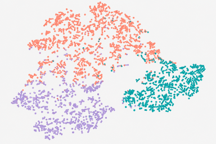
\includegraphics[width=0.45\linewidth]{figure/ACM_clusters.png}
    \caption{t-SNE visualization of learned ACM paper embeddings. Each point represents one paper, and color denotes its class.}
    \label{fig:clustering-acm}
\end{figure}

\begin{figure}[H]
    \centering
    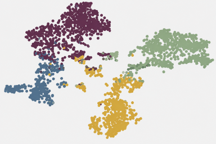
\includegraphics[width=0.45\linewidth]{figure/DBLP_clusters.png}
    \caption{t-SNE visualization of learned DBLP author embeddings. Each point represents one author, and color denotes its research area.}
    \label{fig:clustering-dblp}
\end{figure}

\begin{table}[H]
  \centering
  \caption{Additional clustering-quality diagnostics on DBLP and ACM,
  reported as mean $\pm$ standard deviation over five runs. Best mean
  values are bold.}
  \label{tab:clustering-diagnostic}
  \scriptsize
  \setlength{\tabcolsep}{2.5pt}
  \resizebox{\columnwidth}{!}{%
  \begin{tabular}{llcccc}
    \toprule
    & & \multicolumn{2}{c}{DBLP} & \multicolumn{2}{c}{ACM} \\
    \cmidrule(lr){3-4}
    \cmidrule(lr){5-6}
    \textbf{Group} & \textbf{Model}
    & NMI & ARI
    & NMI & ARI \\
    \midrule

    Hom./hom.
    & GAT
    & $71.50 \pm 0.36$
    & $77.26 \pm 0.48$
    & $57.22 \pm 0.19$
    & $60.47 \pm 0.31$ \\
    \midrule

    \multirow{2}{*}{Het./hom.}
    & NSD
    & $80.21 \pm 0.62$
    & $84.04 \pm 0.43$
    & $62.56 \pm 0.37$
    & $65.02 \pm 0.28$ \\

    & CSNN
    & $81.72 \pm 0.39$
    & $84.25 \pm 0.55$
    & $69.28 \pm 0.45$
    & $71.10 \pm 0.34$ \\
    \midrule

    \multirow{2}{*}{Hom./het.}
    & HAN
    & $79.12 \pm 0.47$
    & $84.76 \pm 0.58$
    & $60.63 \pm 0.22$
    & $64.28 \pm 0.41$ \\

    & PSHGCN
    & $80.38 \pm 0.52$
    & $82.65 \pm 0.36$
    & $71.89 \pm 0.49$
    & $74.31 \pm 0.57$ \\
    \midrule

    \multirow{2}{*}{Het./het.}
    & Hetero2Net
    & $80.54 \pm 0.33$
    & $84.98 \pm 0.46$
    & $70.14 \pm 0.40$
    & $73.42 \pm 0.51$ \\

    & LatGRL
    & $81.36 \pm 0.56$
    & $86.07 \pm 0.38$
    & $72.52 \pm 0.61$
    & $76.75 \pm 0.44$ \\
    \midrule

    Ours
    & \textbf{\method{}}
    & $\mathbf{82.41 \pm 0.35}$
    & $\mathbf{86.52 \pm 0.42}$
    & $\mathbf{75.78 \pm 0.37}$
    & $\mathbf{78.29 \pm 0.31}$ \\
    \bottomrule
  \end{tabular}
  }
\end{table}

\section{Additional Analysis: Diffusion Process of {\method{}}}
\label{sec:diffusion-process-analysis}

We further inspected the training dynamics of \method{} on a controlled four-class
\texttt{FakeHeteroDataset} from torch geometric library. The model was trained with the default synthetic-data settings, and
the visualization includes only nodes with class labels. We recorded the classified-node embedding
layout every five epochs. As shown in Figure~\ref{fig:fakehetero-diffusion-process}, at the beginning of training, nodes from different classes are strongly interleaved. As training proceeds, same-class nodes gradually move toward compact regions, and the
four class-level groups become increasingly separated. This observation suggests that \method{} effectively learns to diffuse information across the heterogeneous graph structure, leading to improved class separability in the learned embeddings.

 \begin{figure}[H]
   \centering
   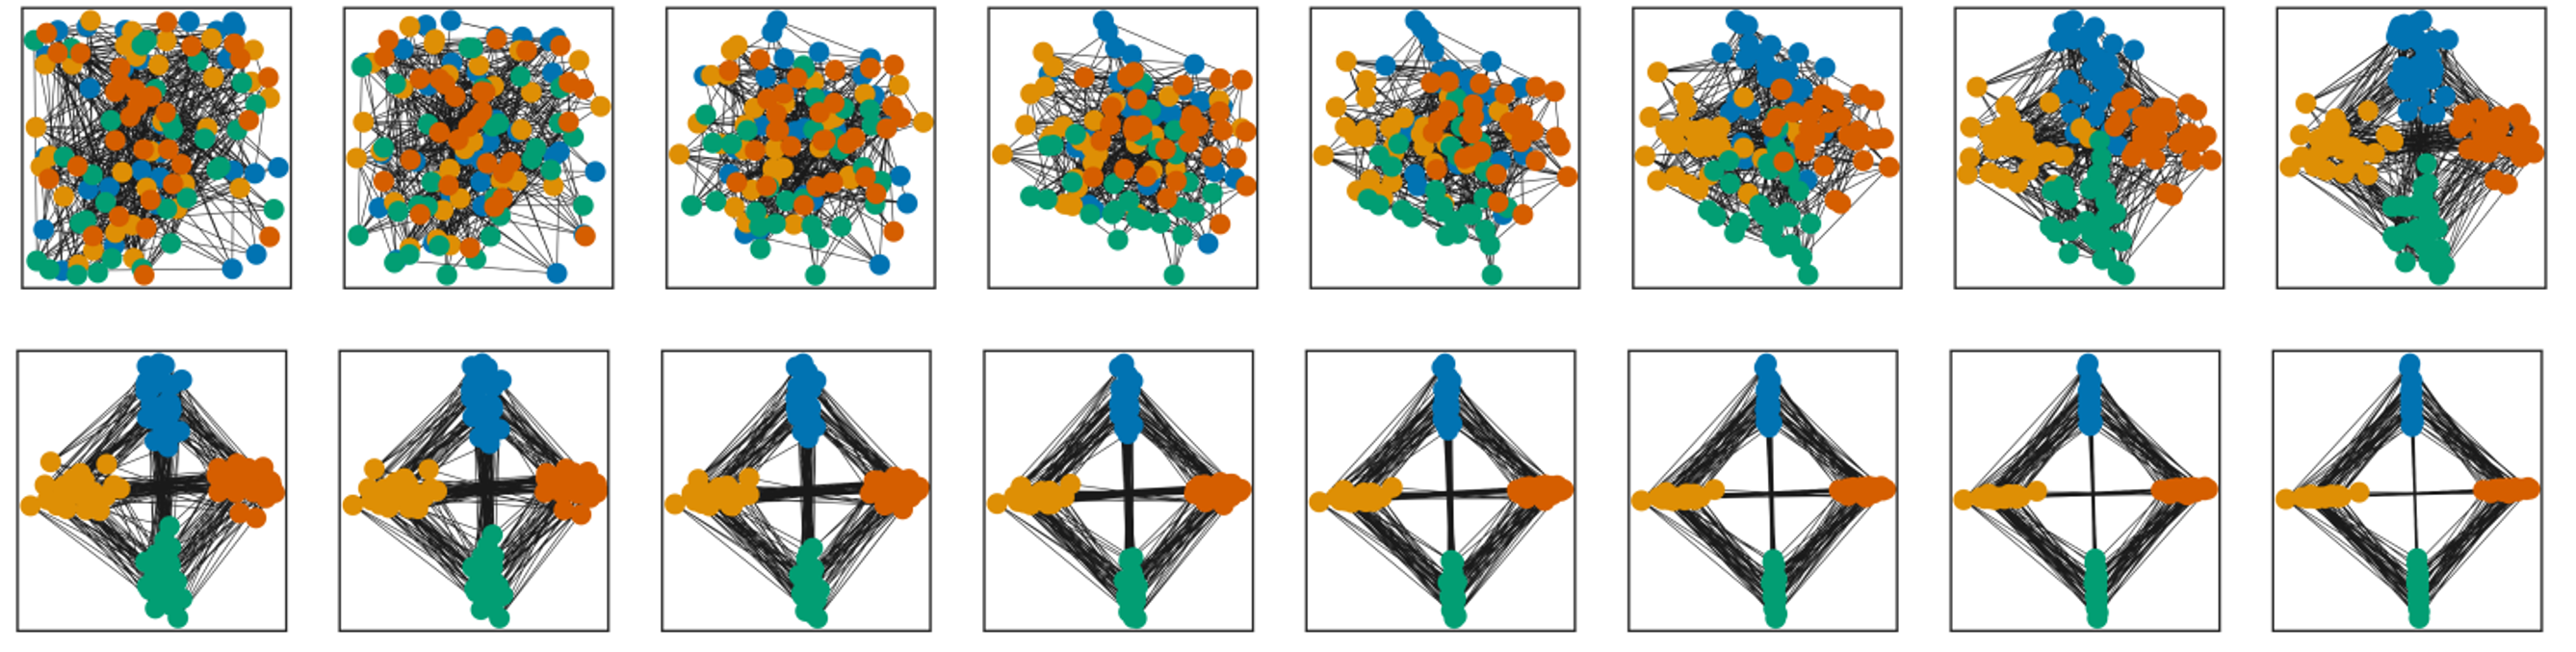
\includegraphics[width=\linewidth]{figure/fakehetero_diffusion_process.png}
   \caption{Training-time diffusion trajectory of \method{} on the four-class
   \texttt{FakeHeteroDataset}. Only labeled nodes are visualized, and consecutive panels are
   separated by five training epochs.}
  \label{fig:fakehetero-diffusion-process}
\end{figure}

\section{Computational Efficiency}

To have a better understanding of the computational cost, we conducted a big-O analysis of \method{}'s, \ampss{}'s, and \sheafcovpool{}'s time and space complexity.

Let $N=|V|$ and
$M=|E|$ be the number of nodes and directed edges, $F$ the number of retained path instances,
and $I=\sum_{f=1}^F \ell_f$ the total edge-face incidences ($\ell_f$ = length of instance
$f$). Let $d$ and $d_r$ denote the stalk and relation-embedding dimensions, and $K$ the number
of Hodge-diffusion steps. Because every edge on a retained path contributes its own edge-to-face
restriction map, the upper Hodge term scales with $I$ rather than $F$ alone.

\paragraph{\ampss{} preprocessing.} Schema construction runs once, before training. With $P$
label-propagation steps, $C_y$ classes, $C_\Sigma$ candidate schemas, $S$ retained schemas,
maximum schema length $L$, and $Q_{\mathrm{type}}$, $Q_{\mathrm{path}}$ the number of typed
and concrete path prefixes visited during enumeration and scoring, preprocessing costs
\[
O\!\left(P(M+N)C_y + Q_{\mathrm{type}} + Q_{\mathrm{path}} + \widehat{F}C_y + C_\Sigma S U + I\right)
\]
time and $O\!\left(M+NC_y+C_\Sigma(L+U)+I\right)$ space, where $\widehat{F}$ instances are
sampled for scoring and $U$ bounds a sampled endpoint set. In the worst case
$Q_{\mathrm{type}}=O(Tb_\Sigma^{L})$ and $Q_{\mathrm{path}}=O((C_\Sigma+S)N\bar{d}^{\,L})$;
in practice \ampss{} caps $C_\Sigma$, $S$, and the number of materialized instances, so the
realized cost is output-sensitive rather than exponential. At inference, the schema gates
cost $O(S)$ per forward pass, and the instance gates (MLP width $h_\beta$) add
$O\!\left(F(2d+d_r)h_\beta\right)$ time and $O(F)$ space.

\paragraph{\method{}.} Table~\ref{tab:complexity} summarizes the per-component
cost of a forward pass, with node-to-edge and edge-to-face MLP widths $h_e$, $h_f$, and
$q(d)=O(d^3)$ for the Householder parameterizations we implement ($O(d^2)$ for
unrestricted dense maps).

\begin{table}[h]
\centering
\scriptsize
\caption{Per-component time and space complexity of the \method{} model. $K$ is the number of diffusion steps}
\label{tab:complexity}
\begin{tabular}{lll}
\toprule
Component & Time & Space \\
\midrule
Node-to-edge & $M\left[(2d+d_r)h_e+h_ed^2+q(d)\right]$ & $Md^2$ \\
Edge-to-face & $(I+F)(d+d_r)h_f+Fh_fd^2$ & $Id^2$ \\
Hodge diffusion & $K(M+I)d^2$ & $(M+I)d^2$ \\
\bottomrule
\end{tabular}
\end{table}

Since node-to-edge and edge-to-face maps are cached and reused across all $K$ diffusion
steps, the full forward pass (excluding readout) costs
\[
O\!\left(Nd_{\mathrm{in}}d + (M+I)d^3 + K(M+I)d^2\right)
\]
once hidden widths scale with $d$, linear in the number of edges and retained edge-face
incidences for fixed $d$. Inference memory is $O\!\left((M+I)d^2+(N+M)d+Fh_f\right)$,
dominated by the cached maps; training adds up to $O(K(N+M)d)$ for the diffusion trajectory.
Note that the edge-to-face encoder holds one hidden vector per path \emph{instance} rather than
one per incidence, since the concatenation in Eq.~\eqref{eq:face-map} collapses the position axis
in its first layer.

\paragraph{\sheafcovpool{} readout.} With $r=3$ node/edge views, projected-descriptor
dimension $f$, pooling width $h_p$, batch size $G$, and $C$ classes, the readout costs
\[
\begin{array}{@{}l@{}}
O\bigl((N+M)[dr^2+r^2h_p+h_pf+f^2] \\
\qquad{}+G[h_pf^2+h_pC]\bigr)
\end{array}
\]
time and
\[
O\!\left((N+M)(dr+f^2)+Gf^2\right)
\]
space. With $r=3$ and $f=8$ fixed, this reduces to $O((N+M)d)$: a linear-time readout
added on top of the model, with no dense Laplacian, node-node covariance, or coarsened graph
ever built.

Furthermore, we reported measured runtime, parameter count, and memory on the ACM node
classification task in Table~\ref{tab:efficiency}.

\begin{table}[H]
  \centering
  \caption{Efficiency comparison on ACM. Best values are bold. Hetsheaf's code is not available, so we used the Hetsheaf-ensemble model reported results in the original paper.}
  \label{tab:efficiency}
  \scriptsize
  \begin{tabular}{lccc}
    \toprule
    \textbf{Model} & Runtime (s) & Parameters & Memory (MB) \\
    \midrule
    R-GCN & \textbf{22.1} & 43M & 1{,}240 \\
    HAN & 28.9 & 2.2M & 1{,}780 \\
    HGT & 1{,}025.8 & 7.2M & 6{,}120 \\
    Sheaf-NSD & 47.6 & \textbf{155K} & \textbf{980} \\
    Hetsheaf & 55.7 & 174K & - \\
    \midrule
    \textbf{\method{}} & 72.1 & 517K & 1120 \\
    \bottomrule
  \end{tabular}
\end{table}

\method{} is not the cheapest model in Table~\ref{tab:efficiency}: R-GCN has the lowest runtime,
and Sheaf-NSD, which models neither relation types nor meta-paths, uses the fewest parameters and
the least memory among the compared models. \method{}'s runtime and parameter count are higher
than Hetsheaf's, the closest heterogeneous sheaf baseline, which we attribute to the additional
edge-to-face maps and \ampss{} schema and instance gates that Hetsheaf does not have. Its memory
footprint nonetheless stays within the same order of magnitude as the other compared models and
well below the heterogeneous transformer baseline HGT, so retaining explicit face-level edge state
does not come at a disproportionate memory cost.

\end{document}

For graph-level prediction, standard pooling operators are
permutation-invariant but not generally invariant to node-wise stalk reparameterisations
\cite{TODO_diffpool,TODO_sagpool,TODO_graphunet,TODO_set2set}, motivating gauge-aware sheaf readouts
such as SheafPool and \sheafcovpool{} \cite{braithwaite2024heterogeneous}.

First, \method{} maps all node types into a shared stalk space and learns relation-aware
restrictions for typed edges. This is needed because heterogeneous features are not directly comparable since each embedding has a different semantic spaces, and heterophilic edges should measure transported disagreement rather than raw similarity. For the observed typed edges, these restrictions provide the node-to-edge geometry used by the later
edge-to-face construction.  After the closure \(1\)-cells are defined, the same coboundary formula is
evaluated on the extended edge set. We therefore map
each type into the common stalk space before comparing adjacent nodes:
\begin{equation}
  h_v^{(0)}
  =\operatorname{Dropout}\!\left[
    \operatorname{GELU}\!\left(
      \operatorname{LN}(W_{\phi(v)}x_v+b_{\phi(v)})+q_{\phi(v)}
    \right)
  \right]\in\R^d ,
  \label{eq:node-encoder}
\end{equation}
where \(W_t,b_t\) are type-specific parameters and \(q_t\) is a learned type embedding.  A learned
node table supplies \(h_v^{(0)}\) when raw attributes are unavailable.  We initialize the diffused
node cochain as \(x^{(0)}=h^{(0)}\), and represent each relation \(r\) by
\(z_r\in\R^{d_r}\).

Given an oriented edge \(e=(u\xrightarrow{r}v)\), two relation-conditioned networks infer
\(F_{u\unlhd e},F_{v\unlhd e}\in\R^{d\times d}\) from
\(h_u^{(0)}\), \(h_v^{(0)}\), and \(z_r\).  Each restriction is scaled orthogonal:
\begin{equation}
  F_{v\unlhd e}=\lambda_{v,e}Q_{v,e},
  \qquad Q_{v,e}^{\transpose}Q_{v,e}=I,
  \qquad \lambda_{v,e}>0 ,
  \label{eq:conformal-map}
\end{equation}
and analogously for \(F_{u\unlhd e}\).  The orthogonal factor aligns local coordinates, while the
positive scale adjusts the strength of the incidence.  On any oriented edge \(e=(u\rightarrow v)\) with available endpoint restrictions, the first coboundary is
\begin{equation}
  (\delta_0x)_e
  =F_{v\unlhd e}x_v-F_{u\unlhd e}x_u .
  \label{eq:delta0}
\end{equation}
Thus, \(\delta_0x\) measures endpoint disagreement after relation-specific transport rather than
raw feature difference. Then, we initialize the edge cochain with a learnable MLP,
\begin{equation}
  s_e^{(0)}
  =\operatorname{MLP}_{\mathrm{init}}\!\left(
    h_u^{(0)}\concat h_v^{(0)}\concat z_r
    \concat(\delta_0h^{(0)})_e
  \right),
  \label{eq:edge-init}
\end{equation}
so \(s^{(0)}\neq\delta_0h^{(0)}\) in general. In the implemented forward pass, this initialization is applied after closure edges have been added, so \(s^{(0)}\) spans both observed edges and closure \(1\)-cells.  This preserves an edge component outside
\(\operatorname{im}\delta_0\) for the subsequent lower- and upper-Hodge interactions.

\\morning


\documentclass[sigconf,anonymous,review]{acmart}

\usepackage{amsthm}
\usepackage{algorithm}
\usepackage{algorithmic}
\usepackage{multirow}

\AtBeginDocument{%
  \providecommand\BibTeX{{Bib\TeX}}}

% Replace the ACM metadata below with the values supplied by the proceedings venue.
\setcopyright{acmlicensed}
\copyrightyear{2026}
\acmYear{2026}
\acmDOI{XXXXXXX.XXXXXXX}
\acmConference[Conference acronym 'XX]{ACM Conference}{Month DD-DD, 2026}{City, Country}
\acmISBN{978-1-4503-XXXX-X/2026/MM}

\newcommand{\R}{\mathbb{R}}
\newcommand{\method}{\textsc{H2S-NN}}
\newcommand{\ampss}{\textsc{AMPSS}}
\newcommand{\sheafcovpool}{\textsc{SheafCovPool}}
\newcommand{\cF}{\mathcal{F}}
\newcommand{\cL}{\mathcal{L}}
\newcommand{\norm}[1]{\left\lVert #1\right\rVert}
\newcommand{\transpose}{\mathsf{T}}
\newcommand{\concat}{\mathbin\Vert}
\newtheorem{proposition}{Proposition}

\title[H2S-NN]{H2S-NN: Heterophilic Heterogeneous Neural Networks with Adaptive Meta-Path Selection}

% Replace the affiliation placeholder before submission.
\author{Peeradon Sarnkaew}
\email{peeradonsarnkaew46@gmail.com}
\affiliation{%
  \institution{Independent Researcher}
  \city{Bangkok}
  \country{Thailand}
}
\renewcommand{\shortauthors}{Sarnkaew}

\begin{document}

\begin{abstract}
Heterogeneous graphs contain many node and relation types, and learning on them raises two problems that are usually handled separately but really occur together. Different relation types carry different meanings, so a single shared update rule can blur information that should stay type-aware; and many of these relations are heterophilic, where connected nodes need not share a label or similar features, so a model that assumes neighbors agree can discard the very signal a relation carries. Meta-paths, typed relations such as author-paper-author, are the standard way to expose multi-hop semantics, but existing methods collapse each into a node-to-node view and lose the path structure a heterophily-aware model could act on. We introduce \method{}, which keeps both problems in view. It compares each edge's endpoints in a shared space, so that a relation-aware disagreement rather than a raw feature gap drives learning, and it retains selected meta-path instances as higher-order structure instead of reducing them to endpoint pairs. To avoid hand-picking meta-paths, \ampss{} learns which schemas and instances matter jointly with the task, while \sheafcovpool{} pools the result for graph classification. Across benchmarks, \method{} leads on node and graph classification and stays competitive on link prediction; ablations confirm that each component contributes.
\end{abstract}

\ccsdesc[500]{Computing methodologies~Neural networks}

\keywords{heterogeneous graph neural networks, heterophily, sheaf neural networks, meta-path discovery, graph pooling}

\maketitle

\section{Introduction}
\label{sec:introduction}


Heterogeneous graphs are a common representation for modeling complex relational structures, such as citation 
networks \cite{liu2014meta} or social interactions \cite{singh2025overview}. Unlike homogeneous graphs, heterogeneous graphs contain multiple types of nodes and edges wwith distinct semantic roles \cite{sun2013mining}. Moreover, many graphs are also heterophilic, where nodes may have different properties. A graph can therefore be both heterogeneous and heterophilic, resulting in a much more complex learning task called heterogeneous heterophilic graph learning, as shown in Figure \ref{fig:het_hom_graph}. Furthermore, modeling graphs under the simplifying assumptions of homogeneity or homophily can obscure important structural and relational patterns. This mismatch provides the model with an incomplete representation of the original graph and may consequently degrade predictive performance \cite{lin2025heterophily}. 

\begin{figure}
  \centering
  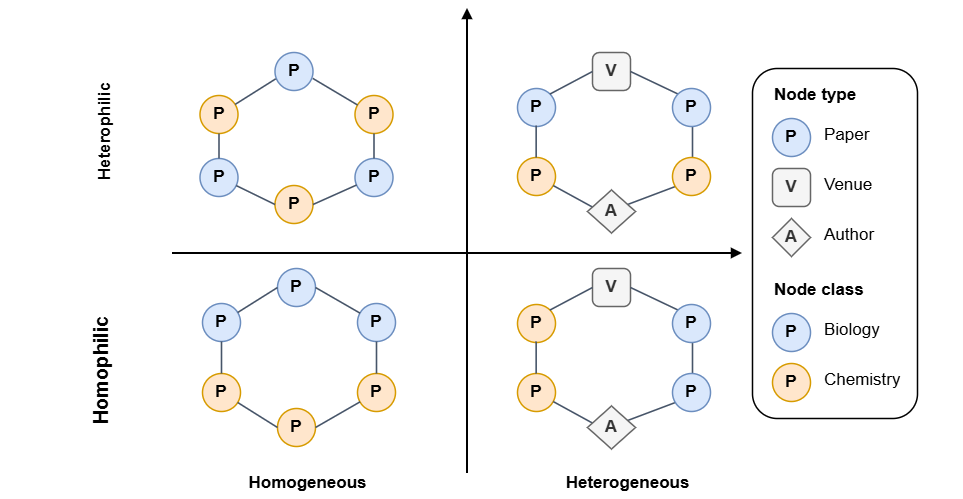
\includegraphics[width=\columnwidth]{figure/Het_HomGraph.drawio.png}
  \caption{An example of heterogeneous heterophilic graph. The graph contains multiple types of nodes and edges, and connected nodes may have different properties.}
  \label{fig:het_hom_graph}
\end{figure}

Many existing methods address either heterogeneous graphs without explicitly considering heterophily \cite{hu2020heterogeneous,mao2023hinormer,he2024spectral,yang2023simple,wang2019heterogeneous,zhang2019heterogeneous} or heterophilic graphs without modeling heterogeneous node and edge types \cite{grover2025spectro,yue2025graph,bodnar2022neural,ribeiro2026cooperative}. Recent methods have begun to address heterogeneous heterophilic graphs through meta-path-based latent subgraphs \cite{lu2026addressing,chen2025adaptive,li2025hetero2net,guo2023homophily,shen2025heterophily,wang2025homophily}, graph rewiring \cite{tao2025cross}, graph transformers \cite{lin2025heterophily}, and sheaf-based mappings \cite{braithwaite2024heterogeneous}. Among these directions, meta-paths can express information that is not contained in either endpoint alone \cite{sun2011pathsim}. For instance, an \texttt{Author-Paper-Author} meta-path describes a co-authorship relation in citation networks, as shown in Figure~\ref{fig:meta_path}. However, existing methods either ignore meta-paths completely, use meta-paths as semantic views, filtered edge sets, or aggregation channels rather than retaining each concrete path instance as part of the propagation structure. For example, an \texttt{A-P-A} meta-path can connect two authors through a shared paper, but after it is converted into an author-author view, the shared paper and the two authorship edges no longer directly shape the propagation operator. This is limiting under heterophily, because whether information should be reinforced or contrasted can depend on the relations along the path, not only on the endpoint connection. This can weaken locality and higher-order information from meta-paths as a part of graph structure.

\begin{figure}
  \centering
  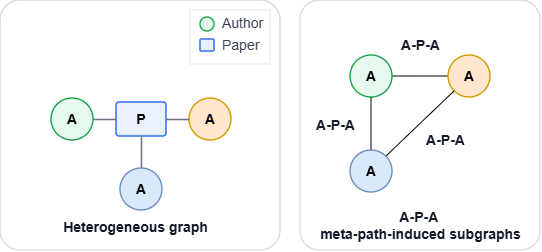
\includegraphics[width=\columnwidth]{figure/meta_path.drawio.png}
  \caption{Illustration of meta-path-induced graph transformation. Under the A-P-A meta-path, authors that share a paper in the original heterogeneous graph are connected in an author-level subgraph.}
  \label{fig:meta_path}
\end{figure}

Manual meta-path specification creates a second bottleneck. Hand-crafted meta-paths are difficult in complex networks, and some useful paths might be ignored \cite{zhong2022pmhgnn,li2024lmsps}. Moreover, datasets often lack such predefined meta-paths. There exists multiple methods for finding useful meta-paths automatically, but they are usually computationally expensive. Some
methods reduce this burden through greedy selection \cite{meng2015discovering}, progressive sampling \cite{li2024lmsps}, searching algorithm \cite{zhang2026mctshgnn,li2023pmmm,li2026amphgnas,sun2025hgsearch}, or reinforcement learning
\cite{zhong2022pmhgnn}.
Although automatic meta-path search reduces reliance on expert knowledge, most methods still select or weight meta-paths at the schema level. However, it is too coarse: a \texttt{PAP} schema may be useful overall, while some concrete \texttt{PAP} instances connect unrelated papers and introduce noise. Schema-level selection must therefore keep noisy instances with useful ones or discard the entire schema. In addition, many search methods select schemas before training the prediction model, so schema choice and instance relevance cannot be refined jointly by the task objective.

To address these challenges, we propose the Heterophilic Heterogeneous Sheaf Neural Network (\method{}), a sheaf–Hodge neural architecture for heterogeneous graphs with heterophily. \method{} represents meta-path instances as higher-order structures by modeling the input graph as a two-dimensional cellular complex. It then learns structural information through sheaf restriction maps and diffusion while preserving the local interactions that give rise to heterophily and heterogeneity.

We further introduce Automatic Meta-Path Selection for Sheaf Neural Networks (\ampss{}), a two-stage component that identifies informative meta-paths during training. \ampss{} learns weights at both the meta-path-schema level and the individual path-instance level.

For graph classification, node and edge sheaf states must be aggregated into a single graph-level representation. Because these states belong to local vector spaces, the readout should be independent of arbitrary choices of local basis. We therefore propose Sheaf Covariance Pooling (\sheafcovpool{}), a gauge- and permutation-invariant readout that aggregates attention-weighted mean and covariance statistics derived from Gram descriptors of node and edge sheaf states. By construction, the resulting graph representation is invariant under the orthogonal transformations associated with \method{}'s restriction maps.

Together, these components form a unified framework for learning meta-paths as higher-order relation in original graphs, heterogeneous, and heterophilic graph representations.




Our main contributions are summarized as follows:
\begin{enumerate}
  \item We introduce \method{}, a heterogeneous sheaf-Hodge framework that retains concrete typed
  path instances as a face-like component on our proposed 2D-cellular graphs, resulting in a learned graph structure that preserves locality without breaking heterophily on heterogeneous graphs.
  \item We propose \ampss{}, a two-stage schema-to-cell selection mechanism that combines
  training-only candidate preselection with differentiable schema- and instance-level refinement
  inside the upper edge Laplacian. This subcomponent allows \method{} to learn which concrete occurrences
  of a schema are useful for the task.
  \item For graph classification, we introduce \sheafcovpool{} as a readout function for graph classification task in \method{}, a gauge-invariant and permutation invariant readout that scores per-node and per-edge learned attention and pools their
  attention-weighted mean and covariance, producing a graph-level representation that is suitable for sheaf neural network.
\end{enumerate}

To this end, we evaluate the framework across node classification, graph classification, and
heterogeneous link prediction. As a result, \method{} achieves the best overall performance across all tasks including node classification, graph classification, and heterogeneous link prediction.

\section{Preliminaries}
\label{sec:background}


\subsection{Heterogeneous graphs}

A heterogeneous graph is a tuple $G=(V,E,\phi,\psi)$, where $V$ and $E$ are the node and edge
sets, $\phi:V\rightarrow\mathcal{T}$ assigns each node a type, and
$\psi:E\rightarrow\mathcal{R}$ assigns each edge a relation type. The realized type sets are
$\mathcal{T}=\{\phi(v):v\in V\}$ and $\mathcal{R}=\{\psi(e):e\in E\}$. The graph is heterogeneous
when it contains more than one node type or more than one relation type, i.e.,
$|\mathcal{T}|>1$ or $|\mathcal{R}|>1$; it reduces to a homogeneous graph when
$|\mathcal{T}|=|\mathcal{R}|=1$ \cite{lu2026addressing}.

\subsection{Homophily and Heterophily}
Homophily describes the tendency of connected nodes to share the same label. For a graph
$G'=(V',E')$ whose endpoint labels are comparable, its edge homophily is
\begin{equation}
  H_{\mathrm{edge}}(G')
  = \frac{1}{|E'|}\sum_{(u,v)\in E'}\mathbf{1}[y_u=y_v],
  \label{eq:background-edge-homophily}
\end{equation}
where $y_u$ is the label of node $u$ and $\mathbf{1}[\cdot]$ is the indicator function
\cite{zhu2020beyond}. Heterophily describes the opposite tendency: adjacent nodes are more likely to have different labels. Larger homophily values indicate stronger label agreement. For heterogeneous graphs, we compute homophily on each meta-path-induced homogeneous subgraph and average across the considered meta-paths \cite{shen2025UHGRL}:
\begin{equation}
    \mathcal{H}
    =
    \frac{1}{|\mathcal{P}|}
    \sum_{p \in \mathcal{P}}
    H_{\mathrm{edge}}(G'_p),
    \label{eq:overall-homophily}
\end{equation}
where $\mathcal{P}$ denotes the set of all considered meta-paths and $G'_p$ is the homogeneous subgraph induced by meta-path $p$.

\subsection{Meta-path}
A meta-path schema of length $\ell$ is a typed relation sequence
\begin{equation}
  \sigma:
  t_0 \xrightarrow{r_1} t_1 \xrightarrow{r_2}\cdots
  \xrightarrow{r_\ell} t_\ell,
  \qquad t_i\in\mathcal{T},\; r_i\in\mathcal{R},
  \label{eq:background-metapath-schema}
\end{equation}
which specifies a composite relation between its endpoint types \cite{sun2011pathsim}. For each
relation $r$, let $A_r\in\{0,1\}^{|V|\times|V|}$ be its adjacency matrix, with
$(A_r)_{uv}=1$ when an edge of type $r$ connects $u$ to $v$. The schema induces the walk-count
matrix
\begin{equation}
  A_\sigma=A_{r_1}A_{r_2}\cdots A_{r_\ell},
  \label{eq:background-metapath-adjacency}
\end{equation}
where $(A_\sigma)_{uv}$ counts the concrete walks from $u$ to $v$ that follow $\sigma$. When
$t_0=t_\ell$, thresholding $A_\sigma$ produces a homogeneous endpoint graph on which
Eq.~\eqref{eq:background-edge-homophily} can be evaluated. For example, the
paper-author-paper schema has $A_{\mathrm{PAP}}=A_{\mathrm{PA}}A_{\mathrm{AP}}$ and connects
papers that share an author. A concrete path instance is an ordered sequence
$f=(v_0,e_1,v_1,\ldots,e_\ell,v_\ell)$ satisfying $\phi(v_i)=t_i$ and $\psi(e_i)=r_i$. Thus,
$\sigma$ describes a type-level pattern, whereas $f$ identifies one occurrence of that pattern in
the observed graph.

\subsection{Cellular Sheaves and Sheaf Neural Networks}

Based sheaf theory, a graph can be viewed as a one-dimensional cellular complex, with nodes as \(0\)-cells and edges as
\(1\)-cells. More general cellular complexes may include higher-dimensional cells, such as
\(2\)-cells bounded by edges, but most sheaf neural networks on graphs operate on the node--edge
complex. We write \(\sigma\unlhd\tau\) when a lower-dimensional cell \(\sigma\) is incident to a
higher-dimensional cell \(\tau\).

A cellular sheaf \(\cF\) assigns each cell \(\sigma\) a vector space, or \emph{stalk},
\(\cF(\sigma)\), and each incident pair \(\sigma\unlhd\tau\) a linear restriction map
\(F_{\sigma\unlhd\tau}:\cF(\sigma)\rightarrow\cF(\tau)\). On a graph \(G=(V,E)\), node and edge
assignments form the cochain spaces
\begin{equation}
  C^0(G,\cF)=\bigoplus_{v\in V}\cF(v),
  \qquad
  C^1(G,\cF)=\bigoplus_{e\in E}\cF(e).
\end{equation}
For an oriented edge \(e=(u\rightarrow v)\), the first coboundary operator
\(\delta_0:C^0(G,\cF)\rightarrow C^1(G,\cF)\) compares endpoint signals after transport into the
edge stalk:
\begin{equation}
  (\delta_0x)_e
  =
  F_{v\unlhd e}x_v-F_{u\unlhd e}x_u.
  \label{eq:prelim-delta0}
\end{equation}
The corresponding sheaf Laplacian is
\(L_0=\delta_0^{\transpose}\delta_0\), with energy
\(x^{\transpose}L_0x=\lVert\delta_0x\rVert_2^2\). When all stalks are one-dimensional and all
restriction maps are identities, \(L_0\) recovers the ordinary graph Laplacian.

Sheaf neural networks can address oversmoothing \cite{alon2020bottleneck}, oversquashing \cite{cai2020note}, and heterophily by replacing direct
feature averaging with diffusion through local stalks and learned restriction maps
\cite{hansen2020sheaf,bodnar2022neural}. Furthermore, other research has extended this idea with
attention, connection Laplacians, positional encodings, nonlinear or polynomial diffusion,
directional variants, and applications beyond ordinary graphs
\cite{barbero2022sheaf,hernandez2024jointdifsheaf,fiorini2025sheaves,mule2025directional,ribeiro2026cooperative,purificato2025sheaf4rec}. HetSheaf further adapts learned
sheaf maps to heterogeneous graphs by conditioning restrictions on node and relation types
\cite{braithwaite2024heterogeneous}.  However, these models
define sheaf structure primarily over observed node-edge incidences. In contrast, \method{}
additionally retains selected meta-path instances as face-like supports and learns edge-to-face maps,
enabling diffusion over an explicit edge cochain.

\section{Methodology}
\label{sec:method}

\subsection{Problem Formulation}

We study supervised learning on directed heterogeneous heterophilic graphs.  The
input is a graph
\(G=(V,E,\phi,\psi,X^{\mathrm{raw}})\), where
\(\phi:V\rightarrow\mathcal{T}\) assigns node types,
\(\psi:E\rightarrow\mathcal{R}\) assigns relation types, and
\(X^{\mathrm{raw}}=\{x_v^{\mathrm{raw}}\}_{v\in V}\) contains type-dependent node features with
\(x_v^{\mathrm{raw}}\in\R^{d_{\phi(v)}}\).  Because different node types may have different feature
spaces, and because adjacent or path-connected nodes may have different labels or dissimilar
attributes, the learner cannot rely on a shared feature encoder or a homophilic aggregation rule.

In addition to the typed graph, the model is given a pool of meta-path schemas
\(\Sigma\), either supplied manually or selected by \ampss{}.  A schema
\(\sigma=(t_0,r_1,t_1,\ldots,r_\ell,t_\ell)\) specifies a valid typed relation sequence, while
\(f=(v_0,e_1,v_1,\ldots,e_\ell,v_\ell)\) denotes one concrete path instance satisfying
\(\phi(v_i)=t_i\) and \(\psi(e_i)=r_i\).  Let \(\mathcal{I}_\sigma\) be the set of observed
instances of schema \(\sigma\), and let
\(\mathcal{I}_\Sigma=\bigcup_{\sigma\in\Sigma}\mathcal{I}_\sigma\).  Unlike methods that collapse a
meta-path into an endpoint-level homogeneous graph, we retain each
\(f\in\mathcal{I}_\Sigma\) as an ordered face-like support over its path edges.

The learning problem is to construct a predictor
\[
  \hat{y}_s
  =
  g_\theta(s;G,\mathcal{I}_\Sigma),
\]
for a task-specific supervised object \(s\).  For node classification, \(s\) is a target node; for
link prediction, \(s\) is a candidate typed node pair; and for graph classification, \(s\) is an
entire graph.  Given labeled training objects \(\mathcal{S}_{\mathrm{train}}\), the parameters are
learned by minimizing
\[
  \min_\theta
  \frac{1}{|\mathcal{S}_{\mathrm{train}}|}
  \sum_{s\in\mathcal{S}_{\mathrm{train}}}
  \mathcal{L}\!\left(g_\theta(s;G,\mathcal{I}_\Sigma),y_s\right).
\]
Thus, the central challenge is to learn type-aware and relation-aware propagation operators that
can use selected meta-path instances as higher-order structure, while avoiding the assumption that
connected nodes should become similar.

\subsection{Framework Overview}

We introduce \method{}, a Heterophilic Heterogeneous Sheaf--Hodge Neural Network for supervised learning on heterogeneous heterophilic graphs. As illustrated in Figure~\ref{fig:pipeline}, the \method{} framework comprises four stages. First, the \emph{Data Input} stage prepares typed node features, relations, and training-only diagnostic statistics. Second, \method{} employs its Automatic Meta-Path Selection subcomponent, \ampss{}, to construct a compact pool of meta-path schemas and learn the importance of their corresponding path instances. Third, the selected paths are incorporated into the sheaf--Hodge encoder, which learns node--edge--face geometry through restriction maps and performs diffusion over node and edge cochains. Finally, \method{} applies a task-specific prediction head. Node classification reads the final states of selected target nodes, link prediction scores pairs of final node representations, and graph classification uses the \sheafcovpool{} subcomponent to aggregate node and edge sheaf states into a graph-level representation.

Thus, \ampss{} serves as the meta-path selection mechanism within \method{}, while \sheafcovpool{} serves as its graph-level readout for graph classification. All tasks share the same underlying sheaf--Hodge encoder and learned geometric operators.

\begin{figure*}[t]
  \centering
  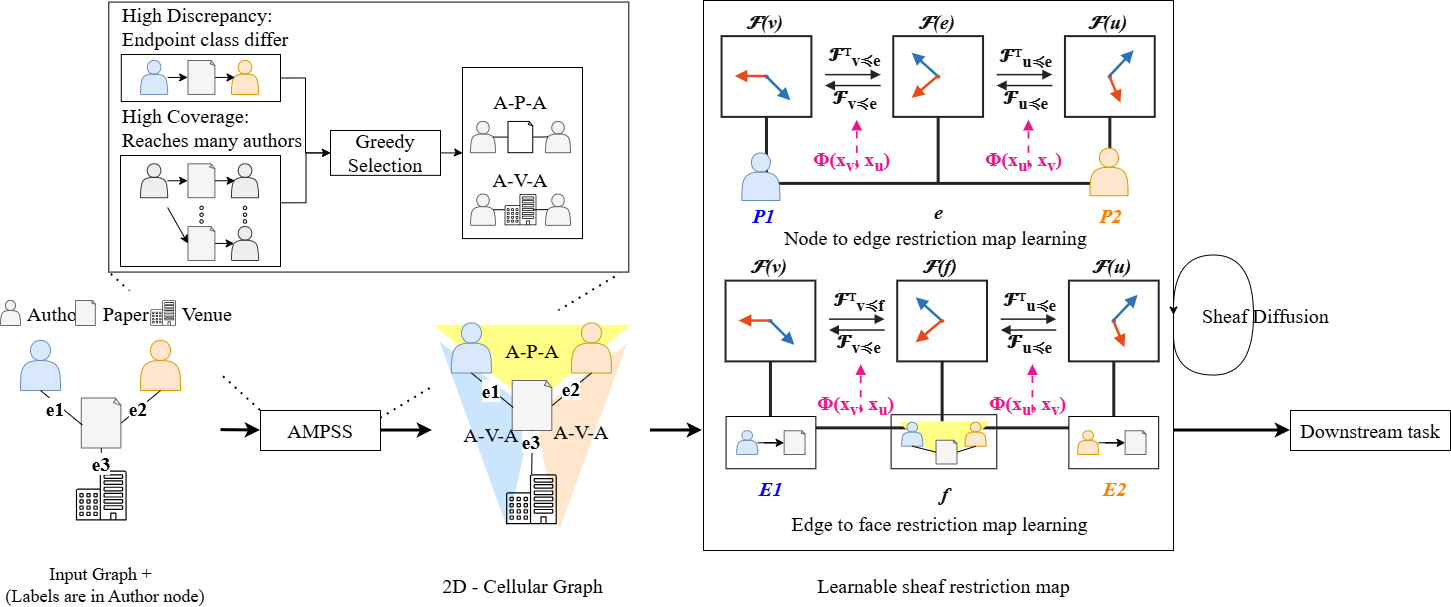
\includegraphics[width=\textwidth]{figure/h2snn_framework_overview.png}
  \caption{Overview of \method{}.  Typed graph data enter a training-only \ampss{} selection stage;
  selected schemas and weighted path instances then parameterize the node-edge-face geometry.
  Node and edge cochains diffuse in parallel before task-specific node, link, or graph prediction,
  with graph classification routed through \sheafcovpool{}.}
  \Description{A left-to-right four-stage diagram.  Data Input feeds AMPSS schema and instance
  selection, which feeds H2S-NN sheaf-Hodge geometry and parallel node and edge diffusion.  The
  output branches to node classification, link prediction, and graph classification through
  SheafCovPool.}
  \label{fig:pipeline}
\end{figure*}



\subsection{Node Stalks and Sheaf Restrictions Initialization}

\method{} First maps all node types into a shared stalk space and learns relation-aware
restrictions for typed edges. This is needed because heterogeneous features occupy different
semantic spaces, while heterophilic edges should measure transported disagreement rather than raw
similarity. For observed typed edges, these restrictions define the node-to-edge geometry later used
by the edge-to-face construction; after closure \(1\)-cells are added, the same coboundary formula is
evaluated on the extended edge set. We therefore map each type into the common stalk space before
comparing adjacent nodes:
\begin{equation}
  h_v^{(0)}
  =\operatorname{Dropout}\!\left[
    \operatorname{GELU}\!\left(
      \operatorname{LN}(W_{\phi(v)}x_v+b_{\phi(v)})+q_{\phi(v)}
    \right)
  \right]\in\R^d ,
  \label{eq:node-encoder}
\end{equation}
where \(W_t,b_t\) are type-specific parameters and \(q_t\) is a learned type embedding.  A learned
node table supplies \(h_v^{(0)}\) when raw attributes are unavailable.  We initialize the diffused
node cochain as \(x^{(0)}=h^{(0)}\), and represent each relation \(r\) by
\(z_r\in\R^{d_r}\).

Given an oriented edge \(e=(u\xrightarrow{r}v)\), two relation-conditioned networks infer
\(F_{u\unlhd e},F_{v\unlhd e}\in\R^{d\times d}\) from
\(h_u^{(0)}\), \(h_v^{(0)}\), and \(z_r\).  Each restriction is scaled orthogonal:
\begin{equation}
  F_{v\unlhd e}=\lambda_{v,e}Q_{v,e},
  \qquad Q_{v,e}^{\transpose}Q_{v,e}=I,
  \qquad \lambda_{v,e}>0 ,
  \label{eq:conformal-map}
\end{equation}
and analogously for \(F_{u\unlhd e}\).  The orthogonal factor aligns local coordinates, while the
positive scale adjusts the strength of the incidence.  On any oriented edge \(e=(u\rightarrow v)\) with available endpoint restrictions, the first coboundary is
\begin{equation}
  (\delta_0x)_e
  =F_{v\unlhd e}x_v-F_{u\unlhd e}x_u .
  \label{eq:delta0}
\end{equation}
Thus, \(\delta_0x\) measures endpoint disagreement after relation-specific transport rather than
raw feature difference. Then, we initialize the edge cochain with a learnable MLP,
\begin{equation}
  s_e^{(0)}
  =\operatorname{MLP}_{\mathrm{init}}\!\left(
    h_u^{(0)}\concat h_v^{(0)}\concat z_r
    \concat(\delta_0h^{(0)})_e
  \right),
  \label{eq:edge-init}
\end{equation}
so \(s^{(0)}\neq\delta_0h^{(0)}\) in general. In the implemented forward pass, this initialization is applied after closure edges have been added, so \(s^{(0)}\) spans both observed edges and closure \(1\)-cells.  This preserves an edge component outside
\(\operatorname{im}\delta_0\) for the subsequent lower- and upper-Hodge interactions.

\subsection{\ampss{}: Adaptive Meta-Path Schema-to-Cell Selection}
\label{sec:ampss}

\ampss{} separates economical structure search from task-driven refinement.  The first stage is a
non-differentiable, training-only construction of a candidate pool; the second stage learns soft
weights for the retained schemas and their concrete instances jointly with \method{}.

\paragraph{Stage I: candidate generation and preselection.}
The first stage constructs a small set of typed higher-order supports before the neural model is
trained.  It does so at the level of the heterogeneous schema rather than by immediately traversing
all concrete node paths.  We first form a directed type graph whose nodes are entity types and whose
directed edges are relation types, e.g., \(P\xrightarrow{\mathrm{writes}^{-1}}A\) and
\(A\xrightarrow{\mathrm{writes}}P\) in a paper--author network.  A bounded depth-first search over
this type graph enumerates valid schema candidates
\(\sigma=(t_0,r_1,t_1,\ldots,r_\ell,t_\ell)\) subject to the allowed length range and, when
required by the task, the start and end target types.  This step therefore proposes only type-valid
relational routes; it does not yet decide that any route is useful.

For each candidate schema, \ampss{} then samples concrete instances in the original graph.  Starting
from nodes of type \(t_0\), it follows the prescribed relation sequence
\((r_1,\ldots,r_\ell)\) and records paths
\(f=(v_0,e_1,v_1,\ldots,e_\ell,v_\ell)\) whose node and edge types match the schema.  Separate
budgets cap the number of candidate schemas, the number of instances expanded from one anchor node,
the number of instances retained for one schema, and the total number of materialized instances.
These caps make the construction economical while still exposing the model to the main typed
relational patterns present in the graph.

Only viable candidates enter preselection.  A schema is viable when sampling produces at least one
unique typed path and its incidence cost
\(c_\sigma=|\mathcal{I}_\sigma|\ell_\sigma\) is compatible with the materialization budget.
Sampling attempts, successful traversals, unique-path counts, and rejected candidates are recorded
for reproducibility and failure diagnosis; they are not separate relevance scores.

We measure relevance through a task-aligned linear probe on an inner split of the outer training
set.  Each viable schema \(\sigma\) contributes a small feature block \(Z_\sigma\).  For node
classification, this block contains the normalized number of sampled paths incident to each target
node, the fraction of unique counterpart nodes, and endpoint evidence propagated from inner-fit
training labels.  For link prediction, it contains direct path counts and source/destination role
evidence propagated from inner-fit positive links.  For graph classification, it records schema
presence and frequency within each inner-training graph.  These quantities are treated jointly as
probe inputs rather than as independent schema-quality claims.

Let \(\mathcal{T}_{\mathrm{fit}}\) and \(\mathcal{T}_{\mathrm{sel}}\) denote the inner probe-fit
and probe-selection partitions, respectively.  For a schema set \(S\), let
\(\cL_{\mathrm{probe}}(S)\) be the task loss on \(\mathcal{T}_{\mathrm{sel}}\) of a regularized
linear probe fitted on \(\mathcal{T}_{\mathrm{fit}}\) using the concatenated blocks
\(\concat_{\sigma\in S}Z_\sigma\).  The marginal task gain of a candidate is
\begin{equation}
  \Delta_{\mathrm{task}}(\sigma\mid S)
  =
  \cL_{\mathrm{probe}}(S)
  -
  \cL_{\mathrm{probe}}(S\cup\{\sigma\}).
  \label{eq:probe-task-gain}
\end{equation}
Thus, a schema is useful only insofar as it improves prediction on training examples not used to
fit the probe.

\ampss{} greedily adds feasible schemas by combining this held-out task gain with one coverage
guard.  Let \(\mathcal{C}_\sigma\) be the target nodes or supervised examples covered by sampled
instances of \(\sigma\), and let \(N_{\mathrm{cov}}\) be the corresponding number of eligible
targets or examples.  With \(\mathcal{C}(S)=\bigcup_{\sigma\in S}\mathcal{C}_\sigma\), the marginal
coverage gain and selection objective are
\begin{equation}
  \begin{aligned}
  \Delta_{\mathrm{cov}}(\sigma\mid S)
  &=
  \frac{|\mathcal{C}(S\cup\{\sigma\})|-|\mathcal{C}(S)|}
       {\max(N_{\mathrm{cov}},1)},\\
  q(\sigma\mid S)
  &=
  \Delta_{\mathrm{task}}(\sigma\mid S)
  +\lambda_{\mathrm{cov}}^{\mathrm{I}}
   \Delta_{\mathrm{cov}}(\sigma\mid S),
  \end{aligned}
  \label{eq:probe-selection-gain}
\end{equation}
subject to \(\sum_{\sigma\in S\cup\{\sigma\}}c_\sigma\leq B_{\mathrm{inc}}\).  Selection stops
when the schema limit is reached, no candidate remains budget-feasible, or the best marginal gain
is non-positive.  The selected schemas are then materialized as ordered path supports together
with the closure pairs used by the node-side correction.  This training-only stage fixes the
candidate support and is intentionally non-differentiable; the next stage decides how strongly
the retained schemas and their individual instances participate in the learned operator.

\paragraph{Stage II: differentiable schema and instance refinement.}
Preselection decides what can be considered; it does not force every retained structure to
contribute equally.  We learn one gate per schema and a state-dependent gate for every path
instance:
\begin{equation}
  \begin{aligned}
  \alpha_\sigma&=\operatorname{sigmoid}(\theta_\sigma),\\
  \beta_f&=\operatorname{sigmoid}\!\left(
    g_\beta(h_{v_0}^{(0)}\concat h_{v_\ell}^{(0)}\concat e_\sigma)
  \right),\\
  w_f&=\alpha_{\sigma(f)}\beta_f .
  \end{aligned}
  \label{eq:gates}
\end{equation}
Here \(e_\sigma\) is a learned schema embedding.  The main probe-based path initializes schema
logits at zero, so \(\alpha_\sigma=0.5\) before learning; \(\beta_f\) then lets two instances of
the same schema have different effects.  During training, partial-schema propagation retains each
schema with probability
\(p_{\mathrm{keep}}\) and rescales a retained gate by \(1/p_{\mathrm{keep}}\), following the
stabilization idea of partial message propagation \cite{li2023pmmm}.

The discovery loss applies complementary pressures rather than a single hard selection rule:
\begin{equation}
  \begin{aligned}
  \cL_{\mathrm{disc}}={}&
  \lambda_s\cL_{\mathrm{sparse\text{-}schema}}
  +\lambda_i\cL_{\mathrm{sparse\text{-}instance}}
  +\lambda_v\cL_{\mathrm{coverage}}\\
  &
  +\lambda_{\mathrm{cost}}\cL_{\mathrm{cost}}
  +\lambda_H\cL_{\mathrm{entropy}} .
  \end{aligned}
  \label{eq:discovery-loss}
\end{equation}
Schema and instance terms discourage diffuse activation; the negative coverage reward discourages
a trivial empty pool; cost suppresses long, frequently instantiated schemas; and entropy
minimization sharpens schema decisions.  These terms refine only the preselected pool and do not
make candidate generation differentiable.  We do not include a redundancy term because the current
metadata do not encode pairwise schema overlap.

\begin{algorithm}[t]
  \caption{\ampss{} candidate preselection and differentiable refinement}
  \label{alg:ampss}
  \begin{algorithmic}[1]
    \REQUIRE Typed relation graph, training split, schema and instance budgets
    \STATE \textbf{Stage I: Candidate generation and training-only preselection}
    \STATE Enumerate bounded typed schemas and sample concrete instances
    \STATE Remove candidates with no unique path or infeasible incidence cost
    \STATE Build task-specific probe blocks from training-only signals
    \STATE Greedily select by probe-loss reduction plus coverage gain under the incidence budget
    \STATE Materialize the selected pool \(\Sigma\) and initialize \(\theta_\sigma=0\)
    \FOR{each training epoch}
      \STATE \textbf{Stage II: Differentiable schema and instance refinement}
      \STATE Use uniform face weights during warm-up
      \STATE Compute \(\alpha_\sigma\), \(\beta_f\), and \(w_f=\alpha_{\sigma(f)}\beta_f\)
      \STATE Apply partial-schema propagation with keep probability \(p_{\mathrm{keep}}\)
      \STATE Run matrix-free sheaf-Hodge diffusion and the task readout
      \STATE Optimize Equation~\ref{eq:loss}
    \ENDFOR
  \end{algorithmic}
\end{algorithm}


\subsection{2D-cellular Sheaf-Hodge Geometry Construction}

The sheaf-Hodge encoder uses the selected path instances to define the cellular support on which
diffusion is performed.  A graph is naturally a \(1\)-dimensional cellular complex: nodes are
\(0\)-cells and typed edges are \(1\)-cells.  \method{} augments this graph with selected
meta-path instances, but it does not collapse a meta-path into an endpoint shortcut.  Instead, a
concrete instance
\[
  f=(v_0,e_1,v_1,\ldots,e_\ell,v_\ell)
\]
is treated as a face-like \(2\)-cell whose boundary contains the ordered path edges.  Since an open
path is not a closed cellular boundary, \method{} also attaches one synthetic closure \(1\)-cell
\(e_{\mathrm{cl}}=(v_\ell\rightarrow v_0)\).  The boundary used by the upper Hodge operator is
therefore
\[
  \partial f=(e_1,\ldots,e_\ell,e_{\mathrm{cl}}).
\]
The closure edge is a modeling device for defining a valid boundary cycle.  It is not an observed
relation and is not interpreted as evidence that the endpoints should be similar.

We write \(\sigma\unlhd\tau\) when a lower-dimensional cell \(\sigma\) is incident to a
higher-dimensional cell \(\tau\).  A cellular sheaf \(\cF\) assigns a local vector space, or
\emph{stalk}, to each cell and a linear restriction map
\(F_{\sigma\unlhd\tau}:\cF(\sigma)\rightarrow\cF(\tau)\) to each incidence.  In \method{}, node,
edge, and face stalks all have dimension \(d\).  The relevant cochain spaces are
\begin{equation}
  C^0(\cF)=\bigoplus_{v\in V}\cF(v),
  \qquad
  C^1(\cF)=\bigoplus_{e\in E\cup E_{\mathrm{cl}}}\cF(e),
  \qquad
  C^2(\cF)=\bigoplus_{f\in\mathcal{I}_{\Sigma}}\cF(f).
\end{equation}
Thus the edge cochain space contains both observed graph edges and closure \(1\)-cells.  This is
important for consistency: the final \(\delta_0\), the initial edge cochain \(s^{(0)}\), \(L_0\),
and the lower part of \(L_1\) are all evaluated on this extended edge set.

For an oriented edge \(e=(u\rightarrow v)\), the first coboundary is
\begin{equation}
  (\delta_0x)_e
  =
  F_{v\unlhd e}x_v-F_{u\unlhd e}x_u .
  \label{eq:background-delta0}
\end{equation}
This quantity is a transported endpoint disagreement, not an average of neighboring features.
It provides the edge-level signal that lets \method{} model heterophily: adjacent or path-connected
nodes may disagree after relation-aware alignment, and this disagreement can itself be informative.
The remaining task is to define the edge-to-face maps so that selected path supports act on edge
cochains without breaking the cochain structure.

\subsection{Path-Supported Edge-Face Geometry}
\label{sec:face-geometry}

The edge-face construction turns each selected path instance into an operator on edge states.  For a
selected \(P\!-\!A\!-\!P\) instance, for example, the two paper-author edges remain the boundary
edges of one face-like support.  The intermediate author is therefore still part of the operator,
rather than disappearing into a paper-paper shortcut.  Operationally, this lets the upper Hodge term
couple disagreements along the whole paper-author-paper pattern.

For a general instance \(f=(v_0,e_1,v_1,\ldots,e_\ell,v_\ell)\), \method{} first predicts one free
map \(A_f\in\R^{d\times d}\) from the ordered path.  Each face group materializes one schema, so all
instances in the group have the same length \(\ell\) and relation sequence
\((r_1,\ldots,r_\ell)\).  The default face encoder concatenates the node states in path order
together with the schema's relation embeddings:
\begin{equation}
  A_f
  =\operatorname{reshape}\!\Big(
    \operatorname{MLP}_{\ell}\big(
      h_{v_0}^{(0)}\concat\cdots\concat h_{v_\ell}^{(0)}
      \concat z_{r_1}\concat\cdots\concat z_{r_\ell}
    \big),\,d,d\Big).
  \label{eq:face-map}
\end{equation}
The order of the path is explicit in this representation, since each node position occupies a
different input slot.  The map \(A_f\) fixes the face stalk's frame for the instance.  It is not used
to independently rescale each boundary edge.

The edge-to-face maps are derived from \(A_f\) by transport.  This constraint is necessary because
the upper Hodge term should measure edge-level curl around a selected support, not create curl from
a pure node-induced gradient.  \method{} therefore carries a transport from the base vertex \(v_0\)
along the path:
\begin{equation}
  \begin{aligned}
  T_{v_0}&=A_f,
  \qquad
  T_{v_i}=T_{v_{i-1}}F_{u\unlhd e_i}^{-1}F_{v\unlhd e_i},\\
  F_{e_i\unlhd f}&=T_{v_{i-1}}F_{u\unlhd e_i}^{-1},
  \end{aligned}
  \label{eq:transport}
\end{equation}
where \(u=v_{i-1}\) and \(v=v_i\).  The inverse is cheap to compute because
Eq.~\eqref{eq:conformal-map} parameterizes node-to-edge maps as a positive scale times an
orthogonal factor, so \(F^{-1}=F^{\transpose}/\lambda^2\).

The closure edge uses the same transported geometry:
\begin{equation}
  F_{v_0\unlhd e_{\mathrm{cl}}}=I,
  \qquad
  F_{v_\ell\unlhd e_{\mathrm{cl}}}=T_{v_0}^{-1}T_{v_\ell},
  \qquad
  F_{e_{\mathrm{cl}}\unlhd f}=A_f .
  \label{eq:closure-maps}
\end{equation}
The middle map is the holonomy of the path,
\(\prod_i F_{u\unlhd e_i}^{-1}F_{v\unlhd e_i}\).  Hence the closure edge introduces no additional
learned relation map.  It only closes the boundary so that the path instance can be used as a
face-like support.

Let \(\eta(e,f)\in\{-1,+1\}\) denote the incidence orientation.  The weighted second coboundary is
\begin{equation}
  (\delta_{1,w}s)_f
  =\sqrt{w_f}\sum_{e\in\partial f}
    \eta(e,f)F_{e\unlhd f}s_e .
  \label{eq:delta1}
\end{equation}
If
\(B_fs=\sum_{e\in\partial f}\eta(e,f)F_{e\unlhd f}s_e\), then the corresponding upper Hodge
contribution is
\begin{equation}
  \delta_{1,w}^{\transpose}\delta_{1,w}
  =\sum_{\sigma\in\Sigma}\sum_{f\in\mathcal{I}_{\sigma}}
    w_f B_f^{\transpose}B_f .
  \label{eq:weighted-up}
\end{equation}
The square root makes the operator linear in the face weight \(w_f\).

\begin{proposition}[Exact cochain condition]
\label{prop:chain}
For every instance whose node sequence is a simple path, the maps of
Eqs.~\eqref{eq:transport}--\eqref{eq:closure-maps} satisfy
\(\delta_{1,w}\delta_0=0\) identically, for every node cochain and every value of the learned
parameters, with no assumption that the sheaf has trivial holonomy.
\end{proposition}

\begin{proof}
By construction \(F_{e_i\unlhd f}F_{u\unlhd e_i}=T_{v_{i-1}}\) and
\(F_{e_i\unlhd f}F_{v\unlhd e_i}=T_{v_i}\).  The \(i\)-th path term of
\(\delta_{1,w}\delta_0x\) is therefore
\(T_{v_i}x_{v_i}-T_{v_{i-1}}x_{v_{i-1}}\), and summing over the path telescopes to
\(T_{v_\ell}x_{v_\ell}-T_{v_0}x_{v_0}\).  The closure maps give
\(F_{e_{\mathrm{cl}}\unlhd f}F_{v_0\unlhd e_{\mathrm{cl}}}=T_{v_0}\) and
\(F_{e_{\mathrm{cl}}\unlhd f}F_{v_\ell\unlhd e_{\mathrm{cl}}}=T_{v_\ell}\), so the closure term
contributes \(T_{v_0}x_{v_0}-T_{v_\ell}x_{v_\ell}\).  The total sum is zero.  The simple-path
condition is required because the transport assigns one map to each node position; a revisited node,
including a coincident endpoint pair, would require two transported values for the same node.
\end{proof}

The chain condition in Proposition~\ref{prop:chain} is not optimized as an additional penalty; it is enforced
by the transported face construction. Its role is to keep
the interpretation of the Hodge decomposition clean: edge signals in \(\operatorname{im}\delta_0\)
come from node potentials, while the upper term acts on edge-level residuals around selected
path-supported cycles.

\begin{figure}[t]
  \centering
  \fbox{\rule{0pt}{4.2cm}\rule{0.94\columnwidth}{0pt}}
  %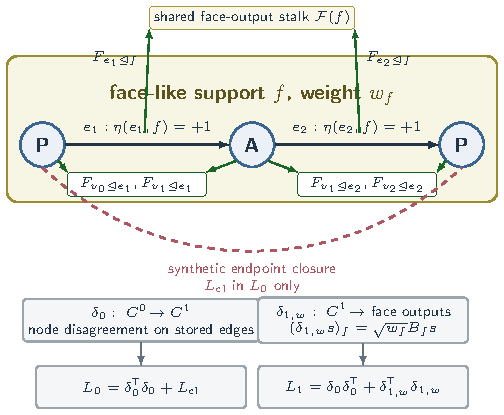
\includegraphics[width=\columnwidth]{figure/h2snn_sheaf_hodge_operator.pdf}
  \caption{AMPSS-selected path instances define a sheaf-Hodge operator. Currently in construction.}
  \label{fig:sheaf-hodge-operator}
\end{figure}

\subsection{Matrix-Free Sheaf-Hodge Diffusion}
\label{sec:closure}

After the restriction maps have been constructed, \method{} applies sheaf-Hodge diffusion to node
and edge cochains.  The two coboundaries define one node operator and one edge operator:
\begin{align}
  L_0x
  &=\delta_0^{\transpose}\delta_0x,
  \label{eq:l0}\\
  L_1s
  &=\underbrace{\delta_0\delta_0^{\transpose}s}_{\text{lower edge term}}
    +\underbrace{\delta_{1,w}^{\transpose}\delta_{1,w}s}_{\text{upper edge term}} .
  \label{eq:l1}
\end{align}
The node operator \(L_0\) acts on transported endpoint disagreements.  The lower edge term in
\(L_1\) compares edge signals through their incident nodes, while the upper edge term couples the
edges around selected path-supported cycles.  Because each closure \(1\)-cell is part of the
extended edge set, it enters \(\delta_0\), \(L_0\), and the lower edge term of \(L_1\) exactly like
other \(1\)-cells.  There is no separate node-side closure correction.

Starting from \(x^{(0)}=h^{(0)}\) and the independently initialized edge cochain \(s^{(0)}\),
\(K\) explicit Euler steps give
\begin{equation}
  \begin{aligned}
  x^{(k+1)}&=x^{(k)}-\eta_0L_0x^{(k)},\\
  s^{(k+1)}&=s^{(k)}-\eta_1L_1s^{(k)},
  \qquad k=0,\ldots,K-1 .
  \end{aligned}
  \label{eq:diffusion}
\end{equation}
The positive step sizes may be learned.  Node and edge cochains evolve in parallel under geometry
built from the same initial node states.  There is no cross-rank recurrence between Euler steps.
Layer normalization then gives the terminal states \(x^\star\) and \(s^\star\), which are passed to
the task-specific readout.

The operators are applied matrix-free.  Rather than constructing global \(Nd\times Nd\) or
\(Md\times Md\) matrices, the implementation batches local restriction maps and aggregates
contributions with indexed sums.  This applies \(\delta_0\), \(\delta_0^{\transpose}\),
\(\delta_{1,w}\), and \(\delta_{1,w}^{\transpose}\) directly on node, edge, and face tensors.

Three implementation boundaries are important.  First, \(\delta_{1,w}\) uses the complete boundary
cycle, consisting of the \(\ell\) path edges and the closure \(1\)-cell.  Second, incidence signs are
represented explicitly.  The currently materialized paths use \(+1\) signs because enumeration
follows stored edge directions and orients the closure edge along the cycle.  Third, the exact
transport argument assumes simple paths, so instances that revisit a node, including coincident
endpoints, are excluded during enumeration.  Under these constraints, the chain condition is a
property of the constructed operator, not a penalty added to the training objective.



\subsection{\sheafcovpool{}}

In sheaf neural diffusion, each node stores its embedding in its own local coordinate system, so embeddings from different nodes cannot simply be pooled together. We therefore introduce \sheafcovpool{}, a readout function that combines node and edge information into a single graph embedding while ignoring these arbitrary coordinate choices. As a result, the graph representation captures the meaningful relationships encoded in \(x^\star\), \(h^{(0)}\), and \(s^\star\), ensuring that the final graph representation reflects the underlying structural information, not the specific basis used to represent each embedding.

The readout first forms small view stacks for nodes and edges.  For a node \(v\), the three views
are its diffused node state, its initial typed state, and the mean state of incident edges.  For an
edge \(e\), the views are the post-diffusion node-to-edge disagreement, the initial disagreement,
and the diffused edge state:
\begin{equation}
  \begin{aligned}
  Z_v^{(0)}
  &=\begin{bmatrix}x_v^\star&h_v^{(0)}&\bar s_v^\star\end{bmatrix}
    \in\R^{d\times3},\\
  Z_e^{(1)}
  &=\begin{bmatrix}
    (\delta_0x^\star)_e&(\delta_0h^{(0)})_e&s_e^\star
  \end{bmatrix}
    \in\R^{d\times3}.
  \end{aligned}
\end{equation}
The Gram descriptor
\[
  G_i^{(r)}=(Z_i^{(r)})^{\transpose}Z_i^{(r)}\in\R^{3\times3},
  \qquad r\in\{0,1\},
\]
records only inner products among these views.  If a local orthogonal gauge changes coordinates as
\(Z_i^{(r)}\mapsto Q_iZ_i^{(r)}\), then \(G_i^{(r)}\) is unchanged.  Thus the classifier sees, for
example, how strongly a node's final state aligns with its initial state or with its incident-edge
summary, but not the arbitrary orientation of the stalk basis.

Nodes and edges play different roles, so separate networks project their descriptors:
\(u_i^{(r)}=\rho_r(\operatorname{vec}G_i^{(r)})\in\R^{d_p}\).  A learned score then selects which
nodes or edges are most informative inside graph \(g\), while the per-graph softmax keeps the
summary permutation invariant:
\begin{equation}
  a_i^{(r)}
  =\frac{\exp(g_r(u_i^{(r)}))}
         {\sum_{j\in\mathcal{C}_r(g)}\exp(g_r(u_j^{(r)}))},
  \qquad
  \mu_r(g)=\sum_{i\in\mathcal{C}_r(g)}a_i^{(r)}u_i^{(r)} .
\end{equation}
Here \(\mathcal{C}_0(g)\) and \(\mathcal{C}_1(g)\) are the nodes and edges of \(g\).  The weighted
mean tells what evidence is present on average, but not whether that evidence is uniform or
concentrated in a few parts of the graph.  \sheafcovpool{} therefore also keeps a weighted
covariance:
\begin{equation}
  \Sigma_r(g)
  =\sum_{i\in\mathcal{C}_r(g)}a_i^{(r)}
    (u_i^{(r)}-\mu_r(g))(u_i^{(r)}-\mu_r(g))^{\transpose}.
\end{equation}
Finally, the graph MLP consumes
\begin{equation}
  \gamma_g=
  \bigl[
  \mu_0(g)\concat\operatorname{triu}(\Sigma_0(g))
  \concat\mu_1(g)\concat\operatorname{triu}(\Sigma_1(g))
  \bigr].
\end{equation}
The result is a single-level readout that uses node and edge evidence, preserves first- and
second-order graph statistics, and remains invariant to node/edge order and orthogonal stalk gauges.

\begin{figure}[t]
  \centering
  \fbox{\rule{0pt}{4.2cm}\rule{0.94\columnwidth}{0pt}}
  %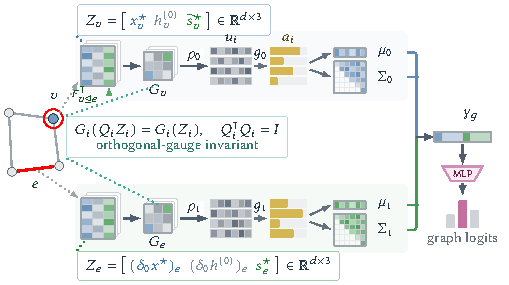
\includegraphics[width=\columnwidth]{figure/sheafcovpool_architecture.pdf}
  \caption{\sheafcovpool{} graph readout. Node and edge view stacks become
  gauge-invariant Gram descriptors; separate attention weights their first and second moments
  before graph classification.}
  \Description{Two parallel node and edge branches.  Each starts with three stalk-valued views,
  forms a Gram descriptor, applies a learned projection and invariant attention, and computes a
  weighted mean and covariance.  Upper-triangular covariance vectors join the means, and the two
  branches concatenate before an MLP outputs graph logits.}
  \label{fig:sheafcovpool}
\end{figure}

\subsection{Training Objective}

\method{} is trained with the supervised task loss and, in auto-discovery mode, the scheduled
\ampss{} discovery objective:
\begin{equation}
  \cL
  =\cL_{\mathrm{task}}
   +\rho(t)\cL_{\mathrm{disc}} .
  \label{eq:loss}
\end{equation}
Here \(\cL_{\mathrm{task}}\) is the task-specific loss: cross-entropy for single-label node and
graph classification, and binary cross-entropy for multi-label classification or link prediction.
The discovery term \(\cL_{\mathrm{disc}}\) combines the schema- and instance-level gate
regularizers used by \ampss{}.  When discovery is disabled, or during the warm-up period before the
gates are active, \(\rho(t)\cL_{\mathrm{disc}}\) is zero.  After warm-up, \(\rho(t)\) either applies
the discovery objective at full strength or increases it linearly, depending on the annealing
setting.  This schedule lets the predictor learn an initial task signal before sparsity, coverage,
and cost pressures begin shaping the schema and instance gates.



\section{Experiments}
\label{sec:experiments}

To ensure generality, we evaluated \method{} on three heterogeneous graph tasks: node classification, link prediction, and graph classification. Model selection was performed using hyperparameter sweeps, and the full per-dataset hyperparameters are listed in Appendix~\ref{app:hyperparameters}. To ensure a fair comparison, we ran each experiment with five random seeds and report the mean performance with standard deviation. The code is available at \url{placeholder_for_code_repository.com}. Results for node classification, link prediction, and graph classification are reported in Tables~\ref{tab:node-cls}, \ref{tab:link-pred}, and~\ref{tab:graph-cls}, respectively. Baselines are grouped by graph type and homophily assumption: Hom./hom., Het./hom., Hom./het., and Het./het., where the first term denotes whether the graph is treated as homogeneous or heterogeneous, and the second denotes whether the method targets homophilic or heterophilic settings.

\subsection{Node Classification}
\label{sec:setup-node}


\paragraph{Datasets.}
On the node classification task, we used three benchmark heterogeneous graph datasets: DBLP \cite{lv2021hgb} and IMDB \cite{lv2021hgb}, and ACM \cite{wang2019han}. The statistics of these datasets are summarized in Table~\ref{tab:node-datasets} given in
Appendix~\ref{app:benchmark-datasets}.


\paragraph{Baselines.} We compared \method{} against four groups of baselines: (i) homogeneous homophilic models, including GCN
\cite{kipf2017gcn}, GAT \cite{velickovic2018gat}, and ChebNetII \cite{he2022chebnetii}; (ii) homogeneous heterophilic models, including NSD
\cite{bodnar2022neural} and CSNN \cite{ribeiro2026cooperative}; (iii)
heterogeneous homophilic models, including HAN \cite{wang2019han}, SeHGNN \cite{yang2023sehgnn},
HiNormer \cite{mao2023hinormer}, and PSHGCN \cite{he2024spectral}; and heterogeneous heterophilic models, including HDHGR \cite{guo2023homophily}, Hetero$^2$Net \cite{li2025hetero2net}, H2SGNN
\cite{lu2026addressing}, HetSheaf \cite{braithwaite2024heterogeneous}, and LatGRL
\cite{shen2025heterophily}.


\paragraph{Evaluation Settings.} We followed the HGB benchmark \cite{lv2021hgb} by using the training/validation/test splits in a ratio of 20\%/20\%/60\% on transductive learning. We used Macro-F1 and Micro-F1 as the evaluation metrics.

\paragraph{Results.}
From the results in Table~\ref{tab:node-cls}, \method{} achieved the best performance on all three benchmark datasets in node classification tasks. \method{} outperforms every baselines in every dataset and every setting. This demonstrates the effectiveness of \method{} in capturing complex heterogeneous graph structures and relationships, leading to improved node classification performance.

\begin{table*}[t]
  \centering
  \caption{Performance on node classification benchmarks reporting in Macro-F1 and Micro-F1. Best values are bold.}
  \label{tab:node-cls}
  \scriptsize
  \resizebox{0.8\textwidth}{!}{%
  \begin{tabular}{llcccccc}
    \toprule
    & &
    \multicolumn{2}{c}{DBLP (59.76)} &
    \multicolumn{2}{c}{ACM (72.39)} &
    \multicolumn{2}{c}{IMDB (50.04)} \\
    \cmidrule(lr){3-4}
    \cmidrule(lr){5-6}
    \cmidrule(lr){7-8}
    \textbf{Group} & \textbf{Model}
    & Macro & Micro
    & Macro & Micro
    & Macro & Micro \\
    \midrule

    \multirow{3}{*}{Hom./hom.}
    & GCN
    & $90.77 \pm 0.76$
    & $90.28 \pm 0.20$
    & $91.63 \pm 0.44$
    & $91.38 \pm 0.39$
    & $62.33 \pm 0.58$
    & $67.69 \pm 0.59$ \\

    & GAT
    & $94.39 \pm 1.03$
    & $92.52 \pm 0.27$
    & $92.07 \pm 0.57$
    & $90.71 \pm 0.21$
    & $62.13 \pm 0.26$
    & $68.09 \pm 0.48$ \\
    
    & ChebNetII
    & $92.89 \pm 1.07$
    & $92.67 \pm 0.50$
    & $91.70 \pm 0.27$
    & $91.59 \pm 0.27$
    & $62.97 \pm 0.66$
    & $68.47 \pm 0.55$ \\

    \midrule

    \multirow{2}{*}{Het./hom.}
    & NSD
    & $92.96 \pm 0.21$
    & $93.42 \pm 0.37$
    & $92.33 \pm 0.78$
    & $92.05 \pm 0.69$
    & $61.61 \pm 0.26$
    & $65.23 \pm 0.51$ \\


    & CSNN
    & $93.73 \pm 0.95$
    & $92.12 \pm 0.19$
    & $93.13 \pm 0.94$
    & $92.81 \pm 0.83$
    & $62.92 \pm 0.34$
    & $62.59 \pm 0.22$ \\


    \midrule

    \multirow{4}{*}{Hom./het.}
    & HAN
    & $91.78 \pm 0.92$
    & $92.24 \pm 0.86$
    & $90.88 \pm 0.67$
    & $91.61 \pm 1.07$
    & $61.95 \pm 0.36$
    & $67.76 \pm 0.51$ \\

    & SeHGNN
    & $95.52 \pm 0.98$
    & $95.48 \pm 0.78$
    & $94.38 \pm 1.00$
    & $94.04 \pm 0.73$
    & $72.01 \pm 0.65$
    & $72.59 \pm 0.18$ \\

    & HiNormer
    & $94.06 \pm 0.40$
    & $94.14 \pm 0.46$
    & $91.87 \pm 0.26$
    & $89.64 \pm 0.39$
    & $64.13 \pm 0.19$
    & $67.53 \pm 0.32$ \\

    & PSHGCN
    & $95.58 \pm 0.80$
    & $95.70 \pm 0.54$
    & $93.66 \pm 0.53$
    & $94.70 \pm 0.39$
    & $71.82 \pm 0.34$
    & $74.34 \pm 0.84$ \\
    \midrule

    \multirow{5}{*}{Het./het.}
    & HDHGR
    & $95.35 \pm 0.81$
    & $95.00 \pm 0.77$
    & $93.99 \pm 0.35$
    & $94.13 \pm 0.87$
    & $59.41 \pm 0.22$
    & $59.63 \pm 0.35$ \\

    & Hetero2Net
    & $93.54 \pm 1.11$
    & $93.54 \pm 0.79$
    & $94.05 \pm 0.71$
    & $92.87 \pm 0.82$
    & $65.34 \pm 0.68$
    & $70.63 \pm 0.69$ \\

    & H2SGNN
    & $95.82 \pm 0.41$
    & $95.11 \pm 0.22$
    & $94.90 \pm 0.49$
    & $94.08 \pm 0.44$
    & $74.23 \pm 0.31$
    & $75.29 \pm 0.86$ \\

    & HetSheaf
    & $93.87 \pm 0.00$
    & $93.77 \pm 0.00$
    & $95.09 \pm 0.00$
    & $94.94 \pm 0.00$
    & $64.65 \pm 0.00$
    & $67.18 \pm 0.00$ \\

    & LatGRL
    & $94.32 \pm 0.44$
    & $94.51 \pm 0.42$
    & $93.47 \pm 0.71$
    & $92.29 \pm 0.43$
    & $58.27 \pm 0.46$
    & $58.81 \pm 0.65$ \\
    \midrule

    Ours
    & \textbf{\method{}}
    & $\mathbf{96.01 \pm 0.58}$
    & $\mathbf{96.31 \pm 0.40}$
    & $\mathbf{95.91 \pm 1.15}$
    & $\mathbf{95.72 \pm 0.68}$
    & $\mathbf{75.05 \pm 0.22}$
    & $\mathbf{76.68 \pm 0.19}$ \\
    \bottomrule
  \end{tabular}%
  }
\end{table*}



\subsection{Graph classification}
\label{sec:setup-graph}
\paragraph{Datasets.}
On the graph classification task, we used four benchmark heterogeneous graph datasets from TUDataset \cite{morris2020tudataset}: biological graphs, including PROTEINS and ENZYMES, and chemical compound graphs, including MUTAG and NCI1. To make those graphs heterogeneous, we treated the node and edge labels supplied by TUDataset as different node and edge types. The detail is  in Table~\ref{tab:graph-datasets} given in Appendix~\ref{app:benchmark-datasets}.



\paragraph{Baselines.} We compared \method{} against four groups of baselines: (i) homogeneous homophilic models, including GCN \cite{kipf2017gcn} and GAT \cite{velickovic2018gat}; (ii) homogeneous heterophilic models, including NSD \cite{bodnar2022neural} and CSNN \cite{ribeiro2026cooperative}; (iii) heterogeneous homophilic models, including HAN \cite{wang2019han} and PSHGCN \cite{he2024spectral}; and (iv) heterogeneous heterophilic models, including HDHGR \cite{guo2023homophily}, Hetero$^2$Net \cite{li2025hetero2net}, H2SGNN \cite{lu2026addressing}, HetSheaf \cite{braithwaite2024heterogeneous}, and LatGRL \cite{shen2025heterophily}.

\paragraph{Evaluation Settings.} Following the graph classification research \cite{zhang2018end, amouzad2024graphunet}, we used 10-fold cross-validation and reported the best evaluation score obtained during training. We used Macro-F1 and Micro-F1 as the evaluation metrics. To ensure a fair comparison, we conducted the experiments with 5 different random seeds, each with 100 epochs for early stopping, and reported the average performance with standard deviation. For the ENZYMES dataset, we used a one-vs-rest (OVR) strategy.

\paragraph{Results.}

From the results in Table~\ref{tab:graph-cls}, \method{} achieved the best performance on all four benchmark datasets in graph classification tasks, tying the MUTAG ceiling and leading PROTEINS, ENZYMES, and NCI1 outright over every compared heterogeneous heterophilic baseline. This suggests that treating the typed node and edge labels as heterogeneous structure, rather than as plain homogeneous graphs with categorical attributes, remains useful even outside the citation- and social-network domains where heterogeneity is usually studied.


\begin{table*}[t]
  \centering
  \caption{Performance on graph classification benchmarks reporting in Macro-F1 and Micro-F1. Best values are bold.}
  \label{tab:graph-cls}
  \scriptsize
  \resizebox{0.8\textwidth}{!}{%
  \begin{tabular}{llcccccccc}
    \toprule
    & &
    \multicolumn{2}{c}{MUTAG} &
    \multicolumn{2}{c}{PROTEINS} &
    \multicolumn{2}{c}{ENZYMES} &
    \multicolumn{2}{c}{NCI1} \\
    \cmidrule(lr){3-4}
    \cmidrule(lr){5-6}
    \cmidrule(lr){7-8}
    \cmidrule(lr){9-10}
    \textbf{Group} & \textbf{Model}
    & Ma. & Mi.
    & Ma. & Mi.
    & Ma. & Mi.
    & Ma. & Mi. \\
    \midrule

    \multirow{2}{*}{Hom./hom.}
    & GCN
    & $89.58 \pm 0.63$
    & $90.00 \pm 0.38$
    & $75.92 \pm 0.55$
    & $79.83 \pm 0.49$
    & $12.75 \pm 0.01$
    & $28.33 \pm 0.03$
    & $64.17 \pm 0.29$
    & $64.96 \pm 0.38$ \\

    & GAT
    & $89.58 \pm 0.06$
    & $90.00 \pm 0.96$
    & $75.27 \pm 0.59$
    & $78.38 \pm 0.71$
    & $14.03 \pm 0.05$
    & $16.55 \pm 0.12$
    & $64.17 \pm 0.27$
    & $64.96 \pm 0.69$ \\
    \midrule

    \multirow{2}{*}{Het./hom.}
    & NSD
    & $\mathbf{100.00 \pm 0.23}$
    & $\mathbf{100.00 \pm 0.31}$
    & $73.60 \pm 0.22$
    & $75.89 \pm 0.49$
    & $33.65 \pm 0.37$
    & $35.00 \pm 0.21$
    & $72.30 \pm 0.31$
    & $72.30 \pm 0.10$ \\

    & CSNN
    & $\mathbf{100.00 \pm 0.39}$
    & $\mathbf{100.00 \pm 0.40}$
    & $76.64 \pm 0.28$
    & $77.92 \pm 0.07$
    & $35.15 \pm 0.07$
    & $37.22 \pm 0.13$
    & $74.11 \pm 0.75$
    & $74.30 \pm 0.80$ \\
    \midrule

    \multirow{2}{*}{Hom./het.}
    & HAN
    & $82.91 \pm 0.61$
    & $85.00 \pm 0.19$
    & $79.19 \pm 0.82$
    & $82.22 \pm 0.50$
    & $46.24 \pm 0.06$
    & $45.02 \pm 0.06$
    & $77.60 \pm 0.43$
    & $77.50 \pm 0.29$ \\

    & PSHGCN
    & $94.88 \pm 0.10$
    & $95.00 \pm 0.42$
    & $70.61 \pm 0.13$
    & $72.32 \pm 0.74$
    & $60.18 \pm 0.24$
    & $58.33 \pm 0.38$
    & $74.17 \pm 0.34$
    & $74.96 \pm 0.37$ \\
    \midrule

    \multirow{5}{*}{Het./het.}
    & HDHGR
    & $84.65 \pm 0.71$
    & $85.00 \pm 0.64$
    & $77.64 \pm 0.83$
    & $81.25 \pm 0.65$
    & $58.27 \pm 0.21$
    & $58.33 \pm 0.64$
    & $79.29 \pm 0.61$
    & $79.32 \pm 0.18$ \\

    & Hetero2Net
    & $89.58 \pm 0.16$
    & $90.00 \pm 0.62$
    & $74.66 \pm 0.69$
    & $78.57 \pm 0.43$
    & $61.53 \pm 0.21$
    & $61.36 \pm 0.49$
    & $63.67 \pm 0.66$
    & $65.45 \pm 0.38$ \\

    & H2SGNN
    & $94.88 \pm 0.09$
    & $95.00 \pm 0.35$
    & $70.61 \pm 0.37$
    & $72.32 \pm 0.14$
    & $62.18 \pm 0.44$
    & $61.31 \pm 0.45$
    & $64.17 \pm 0.06$
    & $64.96 \pm 0.44$ \\

    & HetSheaf
    & $\mathbf{100.00 \pm 0.00}$
    & $\mathbf{100.00 \pm 0.00}$
    & $80.56 \pm 0.00$
    & $82.14 \pm 0.00$
    & $62.35 \pm 0.00$
    & $63.33 \pm 0.00$
    & $79.46 \pm 0.00$
    & $79.46 \pm 0.00$ \\

    & LatGRL
    & $90.88 \pm 0.99$
    & $91.01 \pm 0.11$
    & $71.61 \pm 0.20$
    & $72.32 \pm 0.33$
    & $60.41 \pm 0.09$
    & $60.03 \pm 0.39$
    & $77.98 \pm 0.11$
    & $78.10 \pm 0.41$ \\
    \midrule

    Ours
    & \textbf{\method{}}
    & $\mathbf{100.00 \pm 0.35}$
    & $\mathbf{100.00 \pm 0.83}$
    & $\mathbf{84.44 \pm 0.21}$
    & $\mathbf{86.23 \pm 0.15}$
    & $\mathbf{64.52 \pm 0.56}$
    & $\mathbf{65.10 \pm 0.37}$
    & $\mathbf{81.22 \pm 0.06}$
    & $\mathbf{81.52 \pm 0.20}$ \\
    \bottomrule
  \end{tabular}%
  }
\end{table*}



\subsection{Heterogeneous link prediction}
\label{sec:setup-link}

\paragraph{Datasets.}
On the link prediction task, we used four benchmark heterogeneous graph datasets from HGB \cite{lv2021hgb}: user-item interaction networks, including LastFM, YouTube, and Amazon; and a biological knowledge graph, including PubMed. The statistics of these datasets are summarized in Table~\ref{tab:link-datasets} given in Appendix~\ref{app:benchmark-datasets}.


\paragraph{Baselines.} We compared \method{} against four groups of baselines: (i) homogeneous homophilic models, including GCN \cite{kipf2017gcn} and GAT \cite{velickovic2018gat}; (ii) homogeneous heterophilic models, including NSD \cite{bodnar2022neural} and CSNN \cite{ribeiro2026cooperative}; (iii) heterogeneous homophilic models, including HAN \cite{wang2019han} and PSHGCN \cite{he2024spectral}; and (iv) heterogeneous heterophilic models, including HDHGR \cite{guo2023homophily}, Hetero$^2$Net \cite{li2025hetero2net}, H2SGNN \cite{lu2026addressing}, HetSheaf \cite{braithwaite2024heterogeneous}, and LatGRL \cite{shen2025heterophily}.

\paragraph{Evaluation Settings.} We followed the HGB benchmark \cite{lv2021hgb} by using the training/validation/test splits in a ratio of 81\%/9\%/10\% on transductive learning. We used AUPR and AUROC as the evaluation metrics. The negative sampling strategy is followed the HGB benchmark approach \cite{lv2021hgb} by sampling negative edges for each positive edge in a ratio of 1:1 from the 2-hop neighborhood. 

\paragraph{Results.} From the results in Table~\ref{tab:link-pred}, \method{} achieves the highest mean score on all four link-prediction datasets and all eight reported metrics. The improvement is consistent across both multi-node-type graphs, LastFM and PubMed, and single-node-type multi-relation graphs, Amazon and YouTube. This suggests that the \method{} can capture the complex relationships in heterogeneous heterophilic graphs and \ampss{} path-instance weighting can support link prediction even when heterogeneity is expressed mainly through relation types rather than through multiple node types.

\begin{table*}[t]
  \centering
  \caption{Performance on link prediction benchmarks reporting in AUPR and AUROC. Best values are bold.}
  \label{tab:link-pred}
  \scriptsize
  \setlength{\tabcolsep}{2.5pt}
  \resizebox{0.8\textwidth}{!}
  {%
  \begin{tabular}{llcccccccc}
    \toprule
    & & \multicolumn{2}{c}{LastFM} & \multicolumn{2}{c}{PubMed} & \multicolumn{2}{c}{Amazon} & \multicolumn{2}{c}{YouTube} \\
    \cmidrule(lr){3-4}\cmidrule(lr){5-6}\cmidrule(lr){7-8}\cmidrule(lr){9-10}
    \textbf{Group} & \textbf{Model} & AUPR & AUROC & AUPR & AUROC & AUPR & AUROC & AUPR & AUROC \\
    \midrule

    \multirow{2}{*}{Hom./hom.}
    & GCN
    & $97.06 \pm 0.48$ & $96.96 \pm 0.41$
    & $96.05 \pm 0.52$ & $92.93 \pm 0.36$
    & $92.40 \pm 0.61$ & $89.66 \pm 0.73$
    & $89.30 \pm 0.39$ & $83.26 \pm 0.52$ \\
    & GAT
    & $63.06 \pm 0.27$ & $51.14 \pm 0.19$
    & $96.07 \pm 0.43$ & $93.27 \pm 0.68$
    & $88.62 \pm 0.34$ & $86.10 \pm 0.45$
    & $66.76 \pm 0.31$ & $58.40 \pm 0.22$ \\
    \midrule

    \multirow{2}{*}{Het./hom.}
    & NSD
    & $97.16 \pm 0.71$ & $96.58 \pm 0.65$
    & $96.41 \pm 0.58$ & $93.65 \pm 0.74$
    & $92.63 \pm 0.49$ & $90.04 \pm 0.38$
    & $89.32 \pm 0.43$ & $83.36 \pm 0.57$ \\
    & CSNN
    & $97.99 \pm 0.42$ & $97.75 \pm 0.39$
    & $96.14 \pm 0.30$ & $92.87 \pm 0.29$
    & $92.10 \pm 0.53$ & $89.62 \pm 0.41$
    & $88.64 \pm 0.34$ & $82.97 \pm 0.48$ \\
    \midrule

    \multirow{2}{*}{Hom./het.}
    & HAN
    & $88.26 \pm 0.37$ & $83.32 \pm 0.46$
    & $95.78 \pm 0.49$ & $93.62 \pm 0.62$
    & $95.24 \pm 0.56$ & $93.64 \pm 0.60$
    & $92.46 \pm 0.51$ & $90.10 \pm 0.42$ \\
    & PSHGCN
    & $88.02 \pm 0.44$ & $80.55 \pm 0.50$
    & $97.58 \pm 0.35$ & $93.27 \pm 0.68$
    & $94.28 \pm 0.46$ & $92.34 \pm 0.42$
    & $93.15 \pm 0.63$ & $90.66 \pm 0.58$ \\
    \midrule

    \multirow{5}{*}{Het./het.}
    & HDHGR
    & $97.89 \pm 0.51$ & $97.93 \pm 0.45$
    & $95.03 \pm 0.77$ & $93.15 \pm 0.36$
    & $93.37 \pm 0.40$ & $91.42 \pm 0.59$
    & $91.68 \pm 0.65$ & $88.33 \pm 0.38$ \\
    & Hetero2Net
    & $97.58 \pm 0.29$ & $97.45 \pm 0.61$
    & $94.66 \pm 0.53$ & $92.57 \pm 0.47$
    & $94.71 \pm 0.54$ & $92.34 \pm 0.42$
    & $90.67 \pm 0.70$ & $86.45 \pm 0.41$ \\
    & H2SGNN
    & $97.88 \pm 0.36$ & $97.22 \pm 0.68$
    & $95.22 \pm 0.42$ & $92.32 \pm 0.55$
    & $93.18 \pm 0.61$ & $92.31 \pm 0.50$
    & $90.17 \pm 0.46$ & $88.96 \pm 0.64$ \\
    & LatGRL
    & $96.88 \pm 0.62$ & $96.01 \pm 0.71$
    & $96.61 \pm 0.48$ & $92.32 \pm 0.52$
    & $94.41 \pm 0.43$ & $92.03 \pm 0.57$
    & $89.98 \pm 0.35$ & $88.10 \pm 0.49$ \\
    & HetSheaf
    & $98.51 \pm 0.00$ & $98.00 \pm 0.00$
    & $96.36 \pm 0.00$ & $93.00 \pm 0.00$
    & $93.76 \pm 0.00$ & $91.00 \pm 0.00$
    & $91.27 \pm 0.00$ & $88.00 \pm 0.00$ \\
    \midrule

    Ours
    & \textbf{\method{}}
    & $\mathbf{98.91 \pm 0.37}$ & $\mathbf{98.72 \pm 0.35}$
    & $\mathbf{97.63 \pm 0.41}$ & $\mathbf{96.48 \pm 0.54}$ 
    & $\mathbf{98.53 \pm 0.56}$ & $\mathbf{98.33 \pm 0.44}$
    & $\mathbf{93.95 \pm 0.47}$ & $\mathbf{91.81 \pm 0.33}$  \\
    \bottomrule
  \end{tabular}%
  }
\end{table*}

\section{Discussion}
\label{sec:analysis-results}

\subsection{Ablation Study: Contribution of {\ampss{}}}

To evaluate \ampss{}, we compared the full \method{} on DBLP node classification with variants using no meta-path cells, predefined meta-paths, \ampss{} without the instance-level gate, and the full \ampss{}. As shown in Table~\ref{tab:ablation-schema}, removing meta-path cells decreased Macro-F1/Micro-F1 from $96.01/96.31$ to $93.85/93.72$, confirming that higher-order semantic relations contribute to node classification. Predefined meta-paths recovered most of this loss, while automatically selected schemas achieved comparable performance. The full \ampss{} model performed best after adding the instance-level gate $\beta$, reaching $96.01$ Macro-F1 and $96.31$ Micro-F1. These results suggest that schema-level selection is useful but insufficient: instance-level weighting is needed to filter noisy or uninformative path realizations.

\begin{table}[t]
  \centering
  \caption{Ablation Study of \ampss{} on DBLP node classification.}
  \label{tab:ablation-schema}
  \small
  \begin{tabular}{lcc}
    \toprule
    \textbf{Configuration} & Macro-F1 & Micro-F1 \\
    \midrule
    No meta-path cells & 93.85 & 93.72 \\
    Predefined meta-paths & 95.75 & 96.01 \\
    \ampss{}, $\alpha$ only & 95.88 & 95.92 \\
    \textbf{Full \ampss{}, $\alpha+\beta$} & \textbf{96.01} & \textbf{96.31} \\
    \bottomrule
  \end{tabular}
\end{table}

\subsection{Ablation Study: Contribution of {\sheafcovpool{}}}

To evaluate \sheafcovpool{}, we compared the full \method{} on ENZYMES graph classification with sum, mean, and max pooling over the diffused node state \(x^\star\), SheafPool~\cite{braithwaite2024heterogeneous}, and \sheafcovpool{}. As shown in Table~\ref{tab:ablation-pooling}, the three plain pooling baselines performed similarly. SheafPool improved Macro-F1/Micro-F1 to \(64.05/64.96\), confirming that gauge-invariant readout captures information missed by plain aggregation. \sheafcovpool{} performed best, reaching \(64.52\) Macro-F1 and \(65.10\) Micro-F1. Unlike SheafPool, it pools both node and edge Gram descriptors and retains attention-weighted means together with across-node and across-edge covariances. These results suggest that gauge invariance is useful but not sufficient: second-moment information provides an additional signal for graph-level classification.

\begin{table}[t]
  \centering
  \caption{Ablation study of graph-level readouts on ENZYMES graph classification.}
  \label{tab:ablation-pooling}
  \small
  \begin{tabular}{lcc}
    \toprule
    \textbf{Readout} & Macro-F1 & Micro-F1 \\
    \midrule
    Sum + MLP & 61.25 & 61.79 \\
    Mean + MLP & 61.42 & 62.09 \\
    Max + MLP & 61.38 & 61.62 \\
    SheafPool & 64.05 & 64.96 \\
    \textbf{\sheafcovpool{}} & \textbf{64.52} & \textbf{65.10} \\
    \bottomrule
  \end{tabular}
\end{table}

\section{Conclusion}

To addressed heterogeneous graph learning under heterophily, we introduced \method{}, which treats heterogeneity and heterophily as operator requirements: relation-conditioned node-to-edge maps compare endpoints in a shared local space, while selected meta-path instances remain face-like supports that shape diffusion over an explicit edge cochain instead of being collapsed into induced node-to-node views. Matrix-free Hodge operators propagate node and edge cochains jointly; \ampss{} combines training-only schema preselection with differentiable schema- and instance-level refinement inside the upper edge Laplacian; and \sheafcovpool{} provides a single-level, gauge-invariant readout for graph classification.

The experiments shows that \method{} ranks first among the compared baselines on all three tasks including node-classification, graph-classification , and link prediction on every dataset. Further ablation studies show that the proposed meta-path searching method, \ampss{},  is effective, and that the proposed readout function for graph classification task, \sheafcovpool{}'s, adds useful graph-level signal and improves performance. Together, these results support jointly that modeling type-aware relational structure and heterophily. Altogether, these results indicate complementary benefits from the three components: \method{}
propagates type-aware heterophilic signals through relation-conditioned Hodge operators, \ampss{} subcomponent
learns which schema and path-instance supports should shape the upper edge Laplacian, and
\sheafcovpool{} subcomponent pools gauge-invariant node and edge statistics for graph classification, resulting in a more robust and informative graph neural networks for heterogeneous heterophilic graphs.

\bibliographystyle{ACM-Reference-Format}
\bibliography{references}

\appendix

\section{Data Preparation}
\label{sec:data-prep}
\subsection{Feature Preprocessing}

As feature preprocessing, \method{} uses the same typed input representation for node classification, link prediction,
and graph classification.  We flatten the heterogeneous graph into a single node set and a
directed edge table, while retaining the node-type map \(\phi(v)\) and relation-type map
\(\psi(e)\).  If a node type \(t\) has raw feature width \(d_t\), we store all node features in a
shared padded tensor with width \(D=\max_t d_t\):
\begin{equation}
  \widetilde x_v
  =
  \begin{bmatrix}
    x_v \\ 0_{D-d_{\phi(v)}}
  \end{bmatrix}
  \in\R^D .
  \label{eq:typed-feature-padding}
\end{equation}
The padding is only a storage convention.  The encoder applies the type-specific projection in
Equation~\ref{eq:node-encoder} only to the real feature prefix \(x_v\in\R^{d_{\phi(v)}}\).  For
node types without raw attributes, the same role is played by a learned per-node embedding,
equivalent to applying a linear map to one-hot identity features.  This follows the HGB and
HetSheaf preprocessing convention \cite{lv2021hgb,braithwaite2024heterogeneous}, but keeps the
typed projection inside the model rather than treating the padded tensor as a shared feature
vocabulary.

The only task-dependent preprocessing is used to construct or score candidate schemas for
\ampss{}.  For node classification, we form a training-only label signal
\(Y^{(0)}\in\R^{|V|\times C}\), where \(Y^{(0)}_v\) is the one-hot or multi-hot training label for
\(v\in\mathcal{T}_{\mathrm{train}}\) and is zero otherwise.  Let \(A\) be the directed adjacency
of the flattened graph and let \(D_{\mathrm{in}}\) be the diagonal in-degree matrix.  We propagate
for \(P\) steps with clamping on the training nodes:
\begin{equation}
  Y^{(p+1)}
  =
  \operatorname{row\text{-}norm}
  \!\left(D_{\mathrm{in}}^{-1}A^{\transpose}Y^{(p)}\right),
  \qquad
  Y^{(p+1)}_{\mathcal{T}_{\mathrm{train}}}
  =
  Y^{(0)}_{\mathcal{T}_{\mathrm{train}}}.
  \label{eq:training-label-propagation}
\end{equation}
The resulting \(\widehat Y=Y^{(P)}\) supplies endpoint-evidence channels in the node-classification
probe blocks described in Section~\ref{sec:ampss}.  For link prediction, the same construction is
applied to training-positive endpoint-role indicators rather than class labels.  Graph
classification instead uses per-graph schema presence and frequency.  These task-aligned features
are consumed only by the inner-training probe of Equations~\ref{eq:probe-task-gain}
and~\ref{eq:probe-selection-gain}; they never modify \(\widetilde x\) and never use validation or
test labels or links.  The preprocessing output is therefore the typed graph, the padded typed
feature tensor, and the selected face-like path supports used by the sheaf-Hodge operators.

\subsection{Downstream Readouts}
\label{sec:readouts}

The sheaf-Hodge backbone produces final node states \(x^\star\), final edge states
\(s^\star\), and initial typed node states \(h^{(0)}\).  We leave this backbone unchanged across
tasks and attach a task-specific decoder that maps the relevant final representation to logits.

\paragraph{Node classification.}
For node classification, the readout pools incident edge states back to each node,
\begin{equation}
  \bar s_v^\star
  =
  \begin{cases}
    |E(v)|^{-1}\sum_{e\in E(v)}s_e^\star, & |E(v)|>0,\\
    0, & |E(v)|=0 ,
  \end{cases}
  \label{eq:node-edge-summary}
\end{equation}
and feeds the concatenated node representation into an MLP:
\begin{equation}
  \ell_v
  =
  \operatorname{MLP}_{\mathrm{node}}
  \left(
    x_v^\star\concat h_v^{(0)}\concat\bar s_v^\star
  \right),
  \qquad v\in\mathcal{T}_{\mathrm{target}} .
  \label{eq:node-readout}
\end{equation}
Here \(\ell_v\) denotes the classification logits.  For multiclass node classification we use
cross-entropy loss; for multilabel classification we use binary cross-entropy with logits.

\paragraph{Link prediction.}
For link prediction, the current decoder scores candidate pairs using only the final node states.
Given a candidate pair \((u,v)\), the dot-product decoder returns
\begin{equation}
  \ell_{uv}^{\mathrm{dot}}
  =
  (x_u^\star)^{\transpose}x_v^\star .
  \label{eq:link-dot}
\end{equation}
The concatenation decoder applies an MLP to the endpoint states:
\begin{equation}
  \ell_{uv}^{\mathrm{MLP}}
  =
  \operatorname{MLP}_{\mathrm{link}}
  \left(x_u^\star\concat x_v^\star\right).
  \label{eq:link-mlp}
\end{equation}
The selected decoder output is treated as a raw logit and trained with binary cross-entropy with
logits.

\paragraph{Graph classification.}
For graph classification, \sheafcovpool{} first converts the node and edge cochains of a graph
\(g\) into a permutation- and orthogonal-gauge-invariant summary vector \(\gamma_g\), using the
Gram-descriptor attention and covariance construction described above.  The graph classifier is
then a final MLP:
\begin{equation}
  \ell_g
  =
  \operatorname{MLP}_{\mathrm{graph}}(\gamma_g).
  \label{eq:graph-readout}
\end{equation}
The logits \(\ell_g\) are trained with cross-entropy for single-label graph classification, or
binary cross-entropy with logits for multilabel graph classification.

\section{Hyperparameter Tuning}

For all experiments, we used the same base hyperparameter values for the ACM, DBLP, and IMDB configurations. Dataset-specific overrides are stored in the resolved configuration of each run. The base hyperparameter values are summarized in Table~\ref{tab:hyperparameters}.
Not yet ready
\label{app:hyperparameters}

\begin{table*}[t]
  \centering
  \caption{Base hyperparameter values used in the ACM, DBLP, and IMDB
  configurations. Dataset-specific overrides are stored in the resolved
  configuration of each run.}
  \label{tab:hyperparameters}
  \scriptsize
  
\end{table*}

\section{Benchmark Datasets Explanation}
\label{app:benchmark-datasets}

We evaluated the models on benchmark datasets covering node classification,
link prediction, and graph classification. DBLP, IMDB, and the link-prediction
datasets follow the Heterogeneous Graph Benchmark (HGB)~\cite{lv2021hgb}, while
ACM follows the setup of HAN~\cite{wang2019han}. For graph classification, we
used molecular and biological datasets from TUDataset~\cite{morris2020tudataset};
node and edge labels are treated as node and edge types to instantiate
heterogeneous graph inputs.

\subsection{Node Classification}

\begin{table}[H]
  \centering
  \caption{Node-classification dataset statistics and semantic meta-paths. The \#N and
  \#E columns indicate nodes and edges.}
  \label{tab:node-datasets}
  \scriptsize
  \setlength{\tabcolsep}{2.5pt}
  \resizebox{\columnwidth}{!}
  {%
  \begin{tabular}{lrrrrrll}
    \toprule
    \textbf{Dataset} & \textbf{\#N} & \textbf{\#N types} & \textbf{\#E} &
    \textbf{\#E types} & \textbf{Classes} & \textbf{Target} & \textbf{Meta-paths} \\
    \midrule
    DBLP & 26{,}128 & 4 & 239{,}566 & 6 & 4 & author & APA, APCPA, APTPA \\
    IMDB & 21{,}420 & 4 & 86{,}642 & 6 & 5 & movie & MAM, MDM \\
    ACM & 10{,}942 & 4 & 547{,}806 & 7 & 3 & paper & PAP, PSP \\
    \bottomrule
  \end{tabular}%
  }
\end{table}

\paragraph{DBLP}
is a bibliographic network containing four types of entities: authors,
papers, venues, and terms. These entities are connected through six relation
types, including authorship, publication-venue, paper-term, and author-venue
relations. The prediction target is the author node type, where each author is
assigned to one of four research areas: database systems, data mining,
artificial intelligence, or information retrieval.

\paragraph{IMDB}
is a heterogeneous movie network composed of movies, directors, actors,
and keywords. Its six edge types represent relations such as movie-director,
movie-actor, and movie-keyword associations. The task is multi-label movie
classification, in which a movie may belong to one or more of five genres:
action, comedy, drama, romance, and thriller.

\paragraph{ACM}
is an academic citation network with four node types: papers, authors,
subjects, and terms. Its relations include paper citations, authorship,
paper-subject associations, and paper-term associations. The objective is to
classify papers into three research categories: database systems, wireless
communication, and data mining.

\subsection{Link Prediction}

\begin{table}[H]
  \centering
  \caption{Heterogeneous link-prediction dataset statistics. The \#N and \#E columns
  indicate nodes and edges.}
  \label{tab:link-datasets}
  \scriptsize
  \resizebox{\columnwidth}{!}
  {%
  \begin{tabular}{lrrrrl}
    \toprule
    \textbf{Dataset} & \textbf{\#N} & \textbf{\#N types} & \textbf{\#E} &
    \textbf{\#E types} & \textbf{Target} \\
    \midrule
    LastFM & 20{,}612 & 3 & 141{,}521 & 3 & user-artist \\
    PubMed & 63{,}109 & 4 & 244{,}986 & 10 & disease-disease \\
    YouTube & 2{,}000 & 1 & 1{,}177{,}130 & 5 & user-user \\
    Amazon & 10{,}099 & 1 & 148{,}659 & 2 & product-product \\
    \bottomrule
  \end{tabular}%
  }
\end{table}

\paragraph{LastFM}
is a music-oriented heterogeneous network containing users, artists,
and tags. The graph includes user-artist, user-user, and artist-tag
relations. The link-prediction task determines whether an interaction exists
between a user and an artist.

\paragraph{PubMed}
is a biomedical knowledge graph containing genes, diseases, chemicals,
and species. Ten relation types describe biomedical associations, including
gene-disease, chemical-chemical, and species-disease relations. Evaluation
focuses on predicting links between disease nodes.

\paragraph{YouTube}
is a social interaction graph containing 2,000 user nodes connected by
five distinct types of user interactions. The prediction task is to infer
missing user-user links.

\paragraph{Amazon}
is a product interaction graph with one node type and two relation types. The
task is to predict missing product-product links.

\subsection{Graph Classification}

\begin{table}[H]
  \centering
  \caption{Graph-classification dataset statistics. The Graphs column indicates the
  number of graphs, and \#E indicates edges.}
  \label{tab:graph-datasets}
  \scriptsize
  \setlength{\tabcolsep}{2.5pt}
  \resizebox{\columnwidth}{!}
  {%
  \begin{tabular}{lrrrrl}
    \toprule
    \textbf{Dataset} & \textbf{Graphs} & \textbf{\#N types} & \textbf{\#E} &
    \textbf{\#E types} & \textbf{Target} \\
    \midrule
    MUTAG & 188 & 7 & 7{,}442 & 4 & mutagenicity \\
    PROTEINS & 1{,}113 & 3 & 162{,}088 & 1 & enzyme/non-enzyme \\
    ENZYMES & 600 & 3 & 19{,}580 & 1 & enzyme class \\
    NCI1 & 4{,}110 & 37 & 49{,}205 & 1 & anti-cancer activity \\
    \bottomrule
  \end{tabular}%
  }
\end{table}

\paragraph{MUTAG}
contains 188 molecular graphs representing aromatic and heteroaromatic
nitro compounds. Nodes correspond to seven atom types, while edges encode four
bond types. Each graph is classified according to whether the corresponding
compound exhibits a mutagenic effect.
\paragraph{PROTEINS}
consists of 1,113 protein graphs. Nodes represent secondary-structure
elements belonging to three types, and edges connect elements that are
adjacent either in the amino-acid sequence or in three-dimensional space. The
task is binary classification of proteins into enzyme and non-enzyme classes.
\paragraph{ENZYMES}
contains 600 graph representations of protein tertiary structures
collected from the BRENDA enzyme database. Its nodes describe three types of
secondary-structure elements. Each graph is assigned to one of the six
top-level Enzyme Commission classes.
\paragraph{NCI1}
comprises 4,110 chemical compounds evaluated for their ability to inhibit
the growth of human tumor cell lines. Molecular nodes represent 37 atom types.
The graph-classification objective is to determine whether each compound
exhibits anti-cancer activity.




\section{Additional Experiments: Node Clustering}
\label{sec:additional-clustering}

For a more intuitively comparation and to ensure the performance of keeping locality after training. Although the main experiments evaluate supervised graph-learning tasks, we also used clustering as an additional diagnostic of representation quality. Following the clustering protocol used in the Heterogeneous Graph Attention Network paper \cite{wang2019han}, we ran $k$-means on the learned node embeddings after supervised training. We used DBLP with $k=4$ and ACM with $k=3$, matching the number of classes in each dataset, and set the maximum number of iterations to 300.

We compared \method{} against four groups of baselines: (i) homogeneous homophilic models, including GCN \cite{kipf2017gcn} and GAT \cite{velickovic2018gat}; (ii) homogeneous heterophilic models, including NSD \cite{bodnar2022neural} and CSNN \cite{ribeiro2026cooperative}; (iii) heterogeneous homophilic models, including HAN \cite{wang2019han} and PSHGCN \cite{he2024spectral}; and (iv) heterogeneous heterophilic models, including HDHGR \cite{guo2023homophily}, Hetero$^2$Net \cite{li2025hetero2net}, H2SGNN \cite{lu2026addressing}, HetSheaf \cite{braithwaite2024heterogeneous}, and LatGRL \cite{shen2025heterophily}.

We used Normalized Mutual Information (NMI) and Adjusted Rand Index (ARI) to evaluate clustering quality. We repeated the clustering step over five random seeds and report the mean and standard deviation. As shown in Table~\ref{tab:clustering-diagnostic}, \method{} achieved the highest mean NMI and ARI on both DBLP and ACM. These results suggest that the embeddings learned by \method{} are more separable under this clustering diagnostic. The t-SNE visualizations in Figures~\ref{fig:clustering-acm} and~\ref{fig:clustering-dblp} provide a qualitative view of the learned embeddings \cite{van2008tsne}.

\begin{figure}[H]
    \centering
    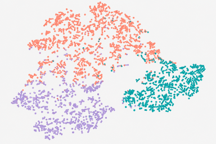
\includegraphics[width=0.45\linewidth]{figure/ACM_clusters.png}
    \caption{t-SNE visualization of learned ACM paper embeddings. Each point represents one paper, and color denotes its class.}
    \label{fig:clustering-acm}
\end{figure}

\begin{figure}[H]
    \centering
    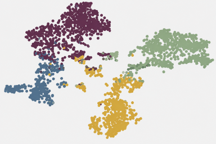
\includegraphics[width=0.45\linewidth]{figure/DBLP_clusters.png}
    \caption{t-SNE visualization of learned DBLP author embeddings. Each point represents one author, and color denotes its research area.}
    \label{fig:clustering-dblp}
\end{figure}

\begin{table}[H]
  \centering
  \caption{Additional clustering-quality diagnostics on DBLP and ACM,
  reported as mean $\pm$ standard deviation over five runs. Best mean
  values are bold.}
  \label{tab:clustering-diagnostic}
  \scriptsize
  \setlength{\tabcolsep}{2.5pt}
  \resizebox{\columnwidth}{!}{%
  \begin{tabular}{llcccc}
    \toprule
    & & \multicolumn{2}{c}{DBLP} & \multicolumn{2}{c}{ACM} \\
    \cmidrule(lr){3-4}
    \cmidrule(lr){5-6}
    \textbf{Group} & \textbf{Model}
    & NMI & ARI
    & NMI & ARI \\
    \midrule

    Hom./hom.
    & GAT
    & $71.50 \pm 0.36$
    & $77.26 \pm 0.48$
    & $57.22 \pm 0.19$
    & $60.47 \pm 0.31$ \\
    \midrule

    \multirow{2}{*}{Het./hom.}
    & NSD
    & $80.21 \pm 0.62$
    & $84.04 \pm 0.43$
    & $62.56 \pm 0.37$
    & $65.02 \pm 0.28$ \\

    & CSNN
    & $81.72 \pm 0.39$
    & $84.25 \pm 0.55$
    & $69.28 \pm 0.45$
    & $71.10 \pm 0.34$ \\
    \midrule

    \multirow{2}{*}{Hom./het.}
    & HAN
    & $79.12 \pm 0.47$
    & $84.76 \pm 0.58$
    & $60.63 \pm 0.22$
    & $64.28 \pm 0.41$ \\

    & PSHGCN
    & $80.38 \pm 0.52$
    & $82.65 \pm 0.36$
    & $71.89 \pm 0.49$
    & $74.31 \pm 0.57$ \\
    \midrule

    \multirow{2}{*}{Het./het.}
    & Hetero2Net
    & $80.54 \pm 0.33$
    & $84.98 \pm 0.46$
    & $70.14 \pm 0.40$
    & $73.42 \pm 0.51$ \\

    & LatGRL
    & $81.36 \pm 0.56$
    & $86.07 \pm 0.38$
    & $72.52 \pm 0.61$
    & $76.75 \pm 0.44$ \\
    \midrule

    Ours
    & \textbf{\method{}}
    & $\mathbf{82.41 \pm 0.35}$
    & $\mathbf{86.52 \pm 0.42}$
    & $\mathbf{75.78 \pm 0.37}$
    & $\mathbf{78.29 \pm 0.31}$ \\
    \bottomrule
  \end{tabular}
  }
\end{table}

\section{Additional Analysis: Diffusion Process of {\method{}}}
\label{sec:diffusion-process-analysis}

We further inspected the training dynamics of \method{} on a controlled four-class
\texttt{FakeHeteroDataset} from torch geometric library. The model was trained with the default synthetic-data settings, and
the visualization includes only nodes with class labels. We recorded the classified-node embedding
layout every five epochs. As shown in Figure~\ref{fig:fakehetero-diffusion-process}, at the beginning of training, nodes from different classes are strongly interleaved. As training proceeds, same-class nodes gradually move toward compact regions, and the
four class-level groups become increasingly separated. This observation suggests that \method{} effectively learns to diffuse information across the heterogeneous graph structure, leading to improved class separability in the learned embeddings.

 \begin{figure}[H]
   \centering
   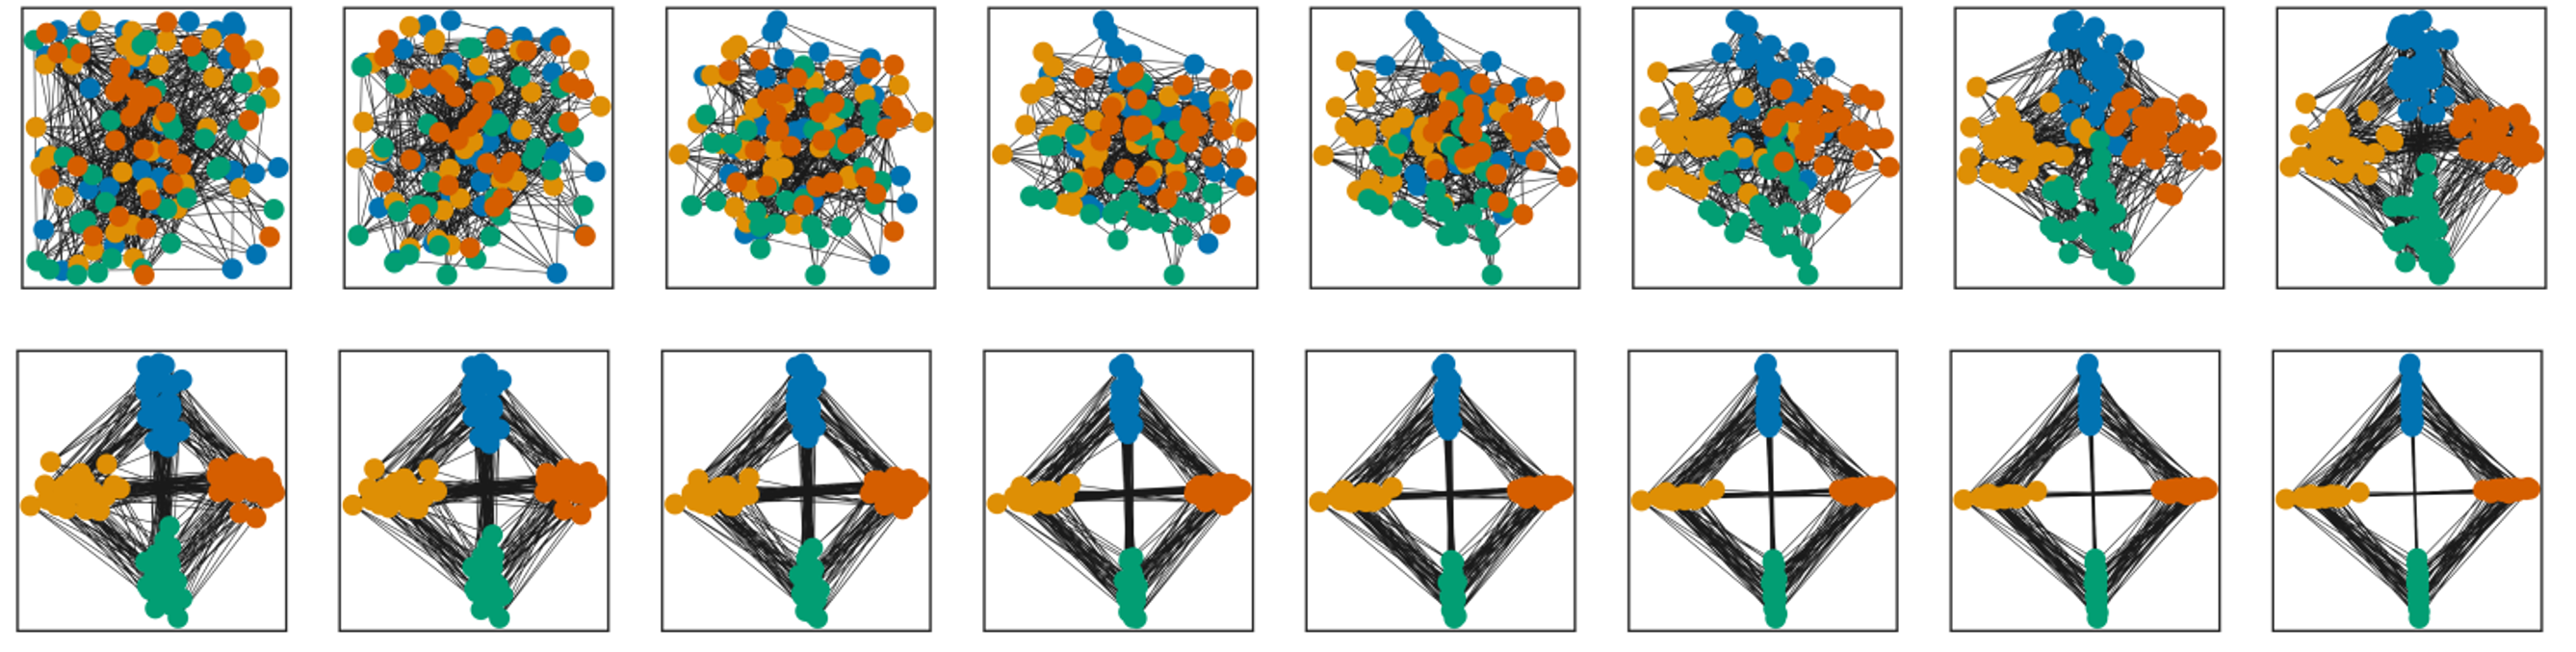
\includegraphics[width=\linewidth]{figure/fakehetero_diffusion_process.png}
   \caption{Training-time diffusion trajectory of \method{} on the four-class
   \texttt{FakeHeteroDataset}. Only labeled nodes are visualized, and consecutive panels are
   separated by five training epochs.}
  \label{fig:fakehetero-diffusion-process}
\end{figure}

\section{Computational Efficiency}

To have a better understanding of the computational cost, we conducted a big-O analysis of \method{}'s, \ampss{}'s, and \sheafcovpool{}'s time and space complexity.

Let $N=|V|$ and
$M=|E|$ be the number of nodes and directed edges, $F$ the number of retained path instances,
and $I=\sum_{f=1}^F \ell_f$ the total edge-face incidences ($\ell_f$ = length of instance
$f$). Let $d$ and $d_r$ denote the stalk and relation-embedding dimensions, and $K$ the number
of Hodge-diffusion steps. Because every edge on a retained path contributes its own edge-to-face
restriction map, the upper Hodge term scales with $I$ rather than $F$ alone.

\paragraph{\ampss{} preprocessing.} Schema construction runs once, before training. With \(P\)
label-propagation steps, \(C_y\) classes, \(C_\Sigma\) viable candidate schemas, \(S\) retained
schemas, maximum schema length \(L\), and \(Q_{\mathrm{type}}\), \(Q_{\mathrm{path}}\) the numbers
of typed and concrete path prefixes visited during enumeration and sampling, preprocessing costs
\[
O\!\left(
P(M+N)C_y + Q_{\mathrm{type}} + Q_{\mathrm{path}}
+ \widehat{F}C_y + C_\Sigma S R N_p S B_Z C_y + I
\right)
\]
time, where \(\widehat{F}\) instances are sampled, \(N_p\) is the inner-probe sample count,
\(B_Z\) bounds one schema's feature width, and \(R\) bounds the linear-probe optimization
iterations.  The last expression is a conservative bound for evaluating up to \(C_\Sigma\)
candidates over \(S\) greedy rounds; incidence-budget rejection reduces the realized number of
probe fits.  Storage is
\(O(M+NC_y+C_\Sigma L+N_pC_\Sigma B_Z+I)\).  In the worst case,
\(Q_{\mathrm{type}}=O(Tb_\Sigma^{L})\) and
\(Q_{\mathrm{path}}=O(C_\Sigma N\bar{d}^{\,L})\);
in practice \ampss{} caps $C_\Sigma$, $S$, and the number of materialized instances, so the
realized cost is output-sensitive rather than exponential. At inference, the schema gates
cost $O(S)$ per forward pass, and the instance gates (MLP width $h_\beta$) add
$O\!\left(F(2d+d_r)h_\beta\right)$ time and $O(F)$ space.

\paragraph{\method{}.} Table~\ref{tab:complexity} summarizes the per-component
cost of a forward pass, with node-to-edge and edge-to-face MLP widths $h_e$, $h_f$, and
$q(d)=O(d^3)$ for the Householder parameterizations we implement ($O(d^2)$ for
unrestricted dense maps).

\begin{table}[h]
\centering
\scriptsize
\caption{Per-component time and space complexity of the \method{} model. $K$ is the number of diffusion steps}
\label{tab:complexity}
\begin{tabular}{lll}
\toprule
Component & Time & Space \\
\midrule
Node-to-edge & $M\left[(2d+d_r)h_e+h_ed^2+q(d)\right]$ & $Md^2$ \\
Edge-to-face & $(I+F)(d+d_r)h_f+Fh_fd^2$ & $Id^2$ \\
Hodge diffusion & $K(M+I)d^2$ & $(M+I)d^2$ \\
\bottomrule
\end{tabular}
\end{table}

Since node-to-edge and edge-to-face maps are cached and reused across all $K$ diffusion
steps, the full forward pass (excluding readout) costs
\[
O\!\left(Nd_{\mathrm{in}}d + (M+I)d^3 + K(M+I)d^2\right)
\]
once hidden widths scale with $d$, linear in the number of edges and retained edge-face
incidences for fixed $d$. Inference memory is $O\!\left((M+I)d^2+(N+M)d+Fh_f\right)$,
dominated by the cached maps; training adds up to $O(K(N+M)d)$ for the diffusion trajectory.
Note that the edge-to-face encoder holds one hidden vector per path \emph{instance} rather than
one per incidence, since the concatenation in Eq.~\eqref{eq:face-map} collapses the position axis
in its first layer.

\paragraph{\sheafcovpool{} readout.} With $r=3$ node/edge views, projected-descriptor
dimension $f$, pooling width $h_p$, batch size $G$, and $C$ classes, the readout costs
\[
\begin{array}{@{}l@{}}
O\bigl((N+M)[dr^2+r^2h_p+h_pf+f^2] \\
\qquad{}+G[h_pf^2+h_pC]\bigr)
\end{array}
\]
time and
\[
O\!\left((N+M)(dr+f^2)+Gf^2\right)
\]
space. With $r=3$ and $f=8$ fixed, this reduces to $O((N+M)d)$: a linear-time readout
added on top of the model, with no dense Laplacian, node-node covariance, or coarsened graph
ever built.

Furthermore, we reported measured runtime, parameter count, and memory on the ACM node
classification task in Table~\ref{tab:efficiency}.

\begin{table}[H]
  \centering
  \caption{Efficiency comparison on ACM. Best values are bold. Hetsheaf's code is not available, so we used the Hetsheaf-ensemble model reported results in the original paper.}
  \label{tab:efficiency}
  \scriptsize
  \begin{tabular}{lccc}
    \toprule
    \textbf{Model} & Runtime (s) & Parameters & Memory (MB) \\
    \midrule
    R-GCN & \textbf{22.1} & 43M & 1{,}240 \\
    HAN & 28.9 & 2.2M & 1{,}780 \\
    HGT & 1{,}025.8 & 7.2M & 6{,}120 \\
    Sheaf-NSD & 47.6 & \textbf{155K} & \textbf{980} \\
    Hetsheaf & 55.7 & 174K & - \\
    \midrule
    \textbf{\method{}} & 72.1 & 517K & 1120 \\
    \bottomrule
  \end{tabular}
\end{table}

\method{} is not the cheapest model in Table~\ref{tab:efficiency}: R-GCN has the lowest runtime,
and Sheaf-NSD, which models neither relation types nor meta-paths, uses the fewest parameters and
the least memory among the compared models. \method{}'s runtime and parameter count are higher
than Hetsheaf's, the closest heterogeneous sheaf baseline, which we attribute to the additional
edge-to-face maps and \ampss{} schema and instance gates that Hetsheaf does not have. Its memory
footprint nonetheless stays within the same order of magnitude as the other compared models and
well below the heterogeneous transformer baseline HGT, so retaining explicit face-level edge state
does not come at a disproportionate memory cost.

\end{document}

\section{Conclusion}
To address heterogeneous graph learning under heterophily, we proposed \method{}, a heterogeneous heterophilic sheaf neural network for supervised learning on typed graphs. The nodes and edges are projected into a shared local space, while selected concrete meta-path instances are retained as path-supported \(2D\)-cells rather than collapsed into induced endpoint-level views. Sheaf-Hodge diffusion with learned restriction maps jointly updates node and edge cochains, allowing selected path-supported \(2D\)-cells to shape local propagation while preserving the ordered, local information carried by each path. We further proposed \ampss{}, which selects task-relevant meta-path schemas and learns an instance-specific weight for each retained path. Finally, we introduced \sheafcovpool{}, a graph-level readout that combines node and incident-edge information into a graph representation invariant to node and edge ordering (permutation invariant) and to independent orthogonal changes of local stalk coordinates, making it suitable for graph-level tasks in sheaf neural networks.
Across the evaluated node-classification, graph-classification, and link-prediction benchmarks, \method{} performs best among the compared methods. The component studies further support the roles of \ampss{} in selecting schemas and path-instance supports and of \sheafcovpool{} in graph-level prediction. Together, these components provide a unified framework for learning from heterogeneous heterophilic graphs while preserving the typed semantic information (heterogeneity), the locality of node and edge information (heterophily), and the graph structure represented by selected concrete meta-path instances as ordered path-supported structures rather than collapsing them into endpoint-only views.



\documentclass[sigconf,anonymous,review]{acmart}

\usepackage{amsthm}
\usepackage{algorithm}
\usepackage{algorithmic}
\usepackage{multirow}

\AtBeginDocument{%
  \providecommand\BibTeX{{Bib\TeX}}}

% Replace the ACM metadata below with the values supplied by the proceedings venue.
\setcopyright{acmlicensed}
\copyrightyear{2026}
\acmYear{2026}
\acmDOI{XXXXXXX.XXXXXXX}
\acmConference[Conference acronym 'XX]{ACM Conference}{Month DD-DD, 2026}{City, Country}
\acmISBN{978-1-4503-XXXX-X/2026/MM}

\newcommand{\R}{\mathbb{R}}
\newcommand{\method}{\textsc{H2S-NN}}
\newcommand{\ampss}{\textsc{AMPSS}}
\newcommand{\sheafcovpool}{\textsc{SheafCovPool}}
\newcommand{\cF}{\mathcal{F}}
\newcommand{\cL}{\mathcal{L}}
\newcommand{\norm}[1]{\left\lVert #1\right\rVert}
\newcommand{\transpose}{\mathsf{T}}
\newcommand{\concat}{\mathbin\Vert}
\newtheorem{proposition}{Proposition}

\title[H2S-NN]{H2S-NN: Heterogeneous Heterophilic Sheaf Neural Network}

% Replace the affiliation placeholder before submission.
\author{Peeradon Sarnkaew}
\email{peeradonsarnkaew46@gmail.com}
\affiliation{%
  \institution{Independent Researcher}
  \city{Bangkok}
  \country{Thailand}
}
\renewcommand{\shortauthors}{Sarnkaew}

\begin{document}

\begin{abstract}
Learning heterogeneous heterophilic graphs requires addressing two properties. First, heterogeneity represents distinct semantic roles through multiple node and relation types in graphs. Second, heterophily means that connected nodes may differ in labels or features, making similarity-based neighbor aggregation unreliable. Another important aspect is the use of meta-path schemas, which expose typed multi-hop semantics. Many existing meta-path methods represent concrete path instances through endpoint-level views and discard the internal path structure and neglect the higher-order information. Therefore, we introduce the Heterogeneous Heterophilic Sheaf Neural Network (\method{}), which retains the observed graph structure and represents meta-path instances as path-supported \(2D\)-cells, thereby preserving graph heterogeneity. In addition, \method{} uses sheaf-Hodge diffusion on sheaf restriction maps to learn graph structure, thereby preserving locality without neglecting heterophily. We also propose Adaptive meta-path schema-to-cell searching and selection (\ampss{}), which uses an auxiliary linear selection model, fitted only on the training data, to select task-relevant meta-path schemas and then learn weights for its concrete path instances. Furthermore, we propose Sheaf covariance pooling (\sheafcovpool{}), which captures graph-level patterns suitable for sheaf neural networks. Across the evaluated node-classification, graph-classification, and link-prediction benchmarks, \method{} achieved the strongest overall performance among the compared methods, supporting its effectiveness for heterogeneous heterophilic graph learning.
\end{abstract}

\ccsdesc[500]{Computing methodologies~Neural networks}

\keywords{heterogeneous graph neural networks, heterophily, sheaf neural networks, meta-path schema searching, graph pooling}

\maketitle

\section{Introduction}
\label{sec:introduction}


Heterogeneous graphs are a common representation for modeling complex relational structures, such as citation 
networks \cite{liu2014meta} or social interactions \cite{singh2025overview}. Unlike homogeneous graphs, heterogeneous graphs contain multiple types of nodes and relations with distinct semantic roles \cite{sun2013mining}. Moreover, many graphs are also heterophilic, meaning that adjacent nodes may have different labels or attributes, making simple similarity-based neighbor aggregation unreliable and prone to oversmoothing. A graph can be both heterogeneous and heterophilic, resulting in a much more complex learning task called heterogeneous heterophilic graph learning, as shown in Figure \ref{fig:het_hom_graph}. Furthermore, modeling graphs under the simplifying assumptions of homogeneity or homophily can obscure important structural and relational patterns. These simplifying assumptions can produce an incomplete representation of the original graph and consequently degrade predictive performance \cite{lin2025heterophily}. 

\begin{figure}
  \centering
  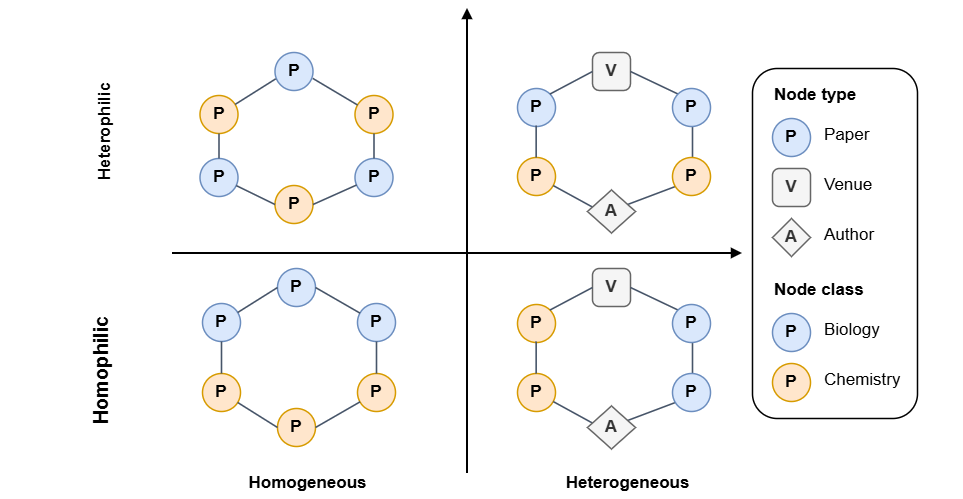
\includegraphics[width=\columnwidth]{figure/Het_HomGraph.drawio.png}
  \caption{An example of a heterogeneous heterophilic graph. The graph contains multiple node and relation types, and adjacent nodes may have different labels or attributes.}
  \label{fig:het_hom_graph}
\end{figure}

Many existing methods address either heterogeneous graphs without explicitly considering heterophily \cite{hu2020heterogeneous,mao2023hinormer,he2024spectral,yang2023simple,wang2019heterogeneous,zhang2019heterogeneous} or heterophilic graphs without modeling heterogeneous node and relation types \cite{grover2025spectro,yue2025graph,bodnar2022neural,ribeiro2026cooperative}. Recent methods have begun to address heterogeneous heterophilic graphs through meta-path-schema-based latent subgraphs \cite{lu2026addressing,chen2025adaptive,li2025hetero2net,guo2023homophily,shen2025heterophily,wang2025homophily}, graph rewiring \cite{tao2025cross}, graph transformers \cite{lin2025heterophily}, and sheaf-based mappings \cite{braithwaite2024heterogeneous}. Another important concept is the use of meta-path schemas. These schemas can express information that is not contained in either node endpoint alone \cite{sun2011pathsim}. For instance, an \texttt{Author-Paper-Author} meta-path schema describes a co-authorship relation in citation networks, as shown in Figure~\ref{fig:meta_path}. However, existing methods either ignore meta-path schemas completely, or use meta-path schemas as semantic views such as filtered edge sets or aggregation channels, rather than retaining each concrete path instance as part of the propagation structure. For example, an \texttt{A-P-A} meta-path schema can connect two authors through a shared paper, but after it is converted into an author-author view, the shared paper and the two authorship edges no longer directly shape the propagation operator. This node-endpoint-only representation is restrictive under heterophily because whether information should be reinforced or contrasted may depend on the relations and intermediate nodes along the path. Collapsing the path can therefore discard local relational structure and higher-order information carried by the concrete path instance.

\begin{figure}
  \centering
  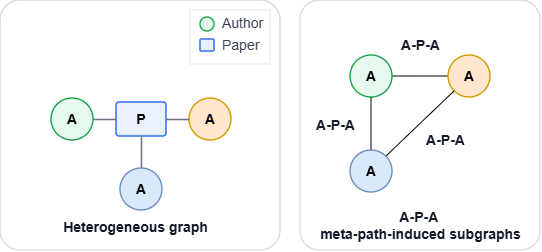
\includegraphics[width=\columnwidth]{figure/meta_path.drawio.png}
  \caption{Illustration of meta-path-schema-induced graph transformation. Under the A-P-A meta-path schema, authors that share a paper in the original heterogeneous graph are connected in an author-level subgraph.}
  \label{fig:meta_path}
\end{figure}

Manually identifying informative meta-path schemas is difficult in complex heterogeneous networks, and datasets often do not provide task-specific meta-path schemas in advance \cite{zhong2022pmhgnn,li2024lmsps}. Hence, there exist multiple methods for finding useful meta-path schemas automatically through greedy selection \cite{meng2015discovering}, progressive sampling \cite{li2024lmsps}, search algorithms \cite{zhang2026mctshgnn,li2023pmmm,li2026amphgnas,sun2025hgsearch}, or reinforcement learning
\cite{zhong2022pmhgnn}. Although automatic meta-path schema search reduces reliance on expert knowledge, most methods still select or weight meta-path schemas at the schema level. However, schema-level weighting is coarse: a \texttt{PAP} schema may be useful overall, while some concrete \texttt{PAP} instances connect unrelated papers and introduce noise. Existing meta-path-schema selection methods may retain noisy instances together with useful ones or discard the entire schema, which does not determine which of its concrete occurrences should influence downstream propagation.

To address these challenges, we propose the \textbf{Heterogeneous Heterophilic Sheaf Neural Network (\method{})}, which retains concrete path instances as path-supported \(2D\)-cells and constructs compatible node-to-edge and edge-to-face geometry for sheaf-Hodge diffusion, thereby preserving the local interactions induced by heterophily and heterogeneity. We further propose \textbf{Adaptive meta-path schema-to-cell searching and selection (\ampss{})}, a two-stage component that selects task-relevant meta-path schemas and learns schema-conditioned weights for its retained concrete path instances. For graph classification, we therefore propose \textbf{Sheaf Covariance Pooling (\sheafcovpool{})}. It aggregates node and edge states through Gram statistics symmetrically, making the readout permutation-invariant and gauge-invariant, i.e., unchanged under independent orthogonal changes of local bases in the node and edge stalks. Together, these components form a unified framework that represents selected concrete path instances as path-supported \(2D\)-cells, which are face-like higher-order structures whose boundaries preserves the ordered path edges. Therefore, the framework learns from heterogeneous heterophilic graphs.

Our main contributions are summarized as follows:
\begin{enumerate}
  \item We introduce a Heterogeneous heterophilic sheaf neural network (\method{}), which retains concrete path instances as path-supported \(2D\)-cells in an augmented path-supported 2D cellular complex, preserving their local relational structure without assuming homophily.
  \item We propose Adaptive meta-path schema-to-cell searching and selection (\ampss{}), a two-stage schema-to-cell selection mechanism that combines training-only schema preselection with differentiable, schema-conditioned instance-level refinement inside the upper edge Laplacian. This subcomponent allows \method{} to learn which concrete occurrences of a selected schema are useful for the task.
  \item We introduce Sheaf Covariance Pooling (\sheafcovpool{}), a graph-level readout that transports incident edge states into node stalks and summarizes node and edge states through attention-weighted Gram means and covariances, yielding a permutation- and gauge-invariant representation.
\end{enumerate}

To this end, we evaluate the framework across node classification, graph classification, and link prediction. As a result, \method{} achieves the best overall performance across all tasks, showing its effectiveness in handling heterogeneous heterophilic graphs.

\section{Preliminaries}
\label{sec:background}


\subsection{Heterogeneous graphs}

A heterogeneous graph is a tuple $G=(V,E,\phi,\psi)$, where $V$ and $E$ are the node and edge
sets, $\phi:V\rightarrow\mathcal{T}$ assigns each node a type, and
$\psi:E\rightarrow\mathcal{R}$ assigns each edge a relation type. The realized type sets are
$\mathcal{T}=\{\phi(v):v\in V\}$ and $\mathcal{R}=\{\psi(e):e\in E\}$. The graph is heterogeneous
when it contains more than one node type or more than one relation type, i.e.,
$|\mathcal{T}|>1$ or $|\mathcal{R}|>1$; it reduces to a homogeneous graph when
$|\mathcal{T}|=|\mathcal{R}|=1$ \cite{lu2026addressing}.

\subsection{Homophily and Heterophily}
Homophily refers to the prevalence of edges between nodes that share the same label. For a graph
$G'=(V',E')$ whose endpoint labels are comparable, its edge homophily is
\begin{equation}
  H_{\mathrm{edge}}(G')
  = \frac{1}{|E'|}\sum_{(u,v)\in E'}\mathbf{1}[y_u=y_v],
  \label{eq:background-edge-homophily}
\end{equation}
where $y_u$ is the label of node $u$ and $\mathbf{1}[\cdot]$ is the indicator function
\cite{zhu2020beyond}. Heterophily describes the opposite prevalence of homophily: adjacent nodes are more likely to have different labels. Larger homophily values indicate stronger label agreement. For heterogeneous graphs, we compute homophily on each meta-path-schema-induced homogeneous subgraph and average across the considered meta-path schemas \cite{shen2025UHGRL}:
\begin{equation}
    \mathcal{H}
    =
    \frac{1}{|\mathcal{P}|}
    \sum_{p \in \mathcal{P}}
    H_{\mathrm{edge}}(G'_p),
    \label{eq:overall-homophily}
\end{equation}
where $\mathcal{P}$ denotes the set of all considered meta-path schemas and $G'_p$ is the homogeneous subgraph induced by meta-path schema $p$.

\subsection{Meta-Path Schemas and Path Instances}
A meta-path schema of length $\ell$ is a typed relation sequence
\begin{equation}
  \pi:
  t_0 \xrightarrow{r_1} t_1 \xrightarrow{r_2}\cdots
  \xrightarrow{r_\ell} t_\ell,
  \qquad t_i\in\mathcal{T},\; r_i\in\mathcal{R},
  \label{eq:background-metapath-schema}
\end{equation}
which specifies a composite relation between its endpoint types \cite{sun2011pathsim}. For each
relation $r$, let $A_r\in\{0,1\}^{|V|\times|V|}$ be its adjacency matrix, with
$(A_r)_{uv}=1$ when a relation of type $r$ connects $u$ to $v$. The schema induces the walk-count
matrix
\begin{equation}
  A_\pi=A_{r_1}A_{r_2}\cdots A_{r_\ell},
  \label{eq:background-metapath-adjacency}
\end{equation}
where $(A_\pi)_{uv}$ counts the concrete walks from $u$ to $v$ that follow $\pi$. When
$t_0=t_\ell$, thresholding $A_\pi$ produces a homogeneous endpoint graph on which
Eq.~\eqref{eq:background-edge-homophily} can be evaluated. For example, as shown in
Figure~\ref{fig:meta_path}, the
paper-author-paper schema has $A_{\mathrm{PAP}}=A_{\mathrm{PA}}A_{\mathrm{AP}}$ and connects
papers that share an author. A concrete path instance is an ordered sequence
$f=(v_0,e_1,v_1,\ldots,e_\ell,v_\ell)$ satisfying $\phi(v_i)=t_i$ and $\psi(e_i)=r_i$. Thus,
$\pi$ describes a type-level pattern, whereas $f$ identifies one occurrence of that pattern in
the observed graph.

\subsection{Cellular Sheaves and Sheaf Neural Networks}

Based on sheaf theory, a graph can be viewed as a one-dimensional cellular complex, with nodes as \(0\)-cells and edges as
\(1\)-cells. More general cellular complexes may include higher-dimensional cells, such as
\(2D\)-cells bounded by edges, but most sheaf neural networks on graphs operate on the node-edge
complex. We write \(c\unlhd\tau\) when a lower-dimensional cell \(c\) is incident to a
higher-dimensional cell \(\tau\).

A cellular sheaf \(\cF\) assigns each cell \(c\) a vector space, or \emph{stalk},
\(\cF(c)\), and each incident pair \(c\unlhd\tau\) a linear restriction map
\(F_{c\unlhd\tau}:\cF(c)\rightarrow\cF(\tau)\). On a graph \(G=(V,E)\), node and edge
assignments form the cochain spaces
\begin{equation}
  C^0(G,\cF)=\bigoplus_{v\in V}\cF(v),
  \qquad
  C^1(G,\cF)=\bigoplus_{e\in E}\cF(e).
\end{equation}
For an oriented edge \(e=(u\rightarrow v)\), the first coboundary operator
\(\delta_0:C^0(G,\cF)\rightarrow C^1(G,\cF)\) compares endpoint signals after transport into the
edge stalk:
\begin{equation}
  (\delta_0x)_e
  =
  F_{v\unlhd e}x_v-F_{u\unlhd e}x_u.
  \label{eq:prelim-delta0}
\end{equation}
The corresponding sheaf Laplacian is
\(L_0=\delta_0^{\transpose}\delta_0\), with energy
\(x^{\transpose}L_0x=\lVert\delta_0x\rVert_2^2\). When all stalks are one-dimensional and all
restriction maps are identities, \(L_0\) recovers the ordinary graph Laplacian.

Sheaf neural networks can address oversmoothing \cite{cai2020note}, oversquashing \cite{alon2021bottleneck}, and heterophily by replacing direct
feature averaging with diffusion through local stalks and learned restriction maps
\cite{hansen2020sheaf,bodnar2022neural}, leading to numerous recent extensions and applications of sheaf neural networks on graphs and in other domains
\cite{barbero2022sheaf,hernandez2024jointdifsheaf,fiorini2025sheaves,mule2025directional,ribeiro2026cooperative,purificato2025sheaf4rec}. HetSheaf further adapts sheaf maps to heterogeneous graphs \cite{braithwaite2024heterogeneous}.  However, these models
define sheaf structure primarily over observed node-edge incidences. In contrast, \method{} retains selected concrete path instances as path-supported \(2D\)-cells in an augmented path-supported \(2D\)-cellular complex and constructs compatible edge-to-face maps, enabling diffusion over an explicit edge cochain.

\section{Methodology}
\label{sec:method}

\subsection{Problem Formulation}

We consider supervised prediction on a directed heterogeneous graph in which neighboring nodes may have different labels or features. The graph is formulated as
\(G=(V,E,\phi,\psi,X^{\mathrm{raw}})\), where
\(\phi:V\rightarrow\mathcal{T}\) assigns node types,
\(\psi:E\rightarrow\mathcal{R}\) assigns relation types, and
\(X^{\mathrm{raw}}=\{x_v^{\mathrm{raw}}\}_{v\in V}\) contains type-dependent node features with
\(x_v^{\mathrm{raw}}\in\R^{d_{\phi(v)}}\). 

The model is given meta-path schemas
\(\pi\), either supplied manually or selected by \ampss{}.  A schema
\(\pi=(t_0,r_1,t_1,\ldots,r_\ell,t_\ell)\) specifies a valid typed relation sequence, while
\(f=(v_0,e_1,v_1,\ldots,e_\ell,v_\ell)\) denotes one concrete path instance satisfying
\(\phi(v_i)=t_i\) and \(\psi(e_i)=r_i\).  Let \(\mathcal{I}_\pi\) be the set of observed
instances of schema \(\pi\), and let
\(\mathcal{I}_\Sigma=\bigcup_{\pi\in\Sigma}\mathcal{I}_\pi\).  Unlike methods that collapse a
meta-path schema into an endpoint-level homogeneous graph, we represent each retained path instance as a path-supported \(2\)-cell: a face-like higher-order structure whose boundary preserves the ordered path
edges and includes a synthetic closure edge introduced below.

The learning problem is to construct a predictor
\[
  \hat{y}_o
  =
  g_\theta(o;G,\mathcal{I}_\Sigma),
\]
for a task-specific supervised object \(o\).  For node classification, \(o\) is a target node; for
link prediction, \(o\) is a candidate typed node pair; and for graph classification, \(o\) is an
entire graph.  Given labeled training objects \(\mathcal{S}_{\mathrm{train}}\), the parameters are
learned by minimizing
\[
  \min_\theta
  \frac{1}{|\mathcal{S}_{\mathrm{train}}|}
  \sum_{o\in\mathcal{S}_{\mathrm{train}}}
  \mathcal{L}\!\left(g_\theta(o;G,\mathcal{I}_\Sigma),y_o\right).
\]

\(\cL\) is cross-entropy for single-label node and graph classification,
and binary cross-entropy for multilabel node classification and link prediction. Thus, the central challenge is to learn type-aware and relation-aware propagation operators that can use selected concrete path instances as path-supported \(2D\)-cells on heterogeneous heterophilic graphs.

\subsection{Overview}

We introduce \method{}, a Heterogeneous heterophilic sheaf neural network, for supervised learning on heterogeneous heterophilic graphs. As shown in Figure~\ref{fig:pipeline}, \method{} consists of four stages. First, \emph{Input graph preprocessing} prepares typed graph features and relations. Second, \ampss{} generates candidate meta-path schemas using bounded
depth-first search, selects a task-relevant schema set (Stage I), and learns schema-conditioned weights for its retained concrete instances (Stage II). Third, the \emph{Sheaf-Hodge Encoding} stage incorporates the selected concrete path instances to learn node-to-edge and path-supported edge-to-face geometry. Finally, the \emph{Sheaf-Hodge Diffusion} stage evolves the node and edge cochains to obtain their final representations, with the proposed \sheafcovpool{} provided as the graph-level readout. Together, these stages allow \method{} to retain the local relational structure of selected concrete path instances while learning from heterogeneous graphs under heterophily.

\begin{figure*}[htbp]
  \centering
  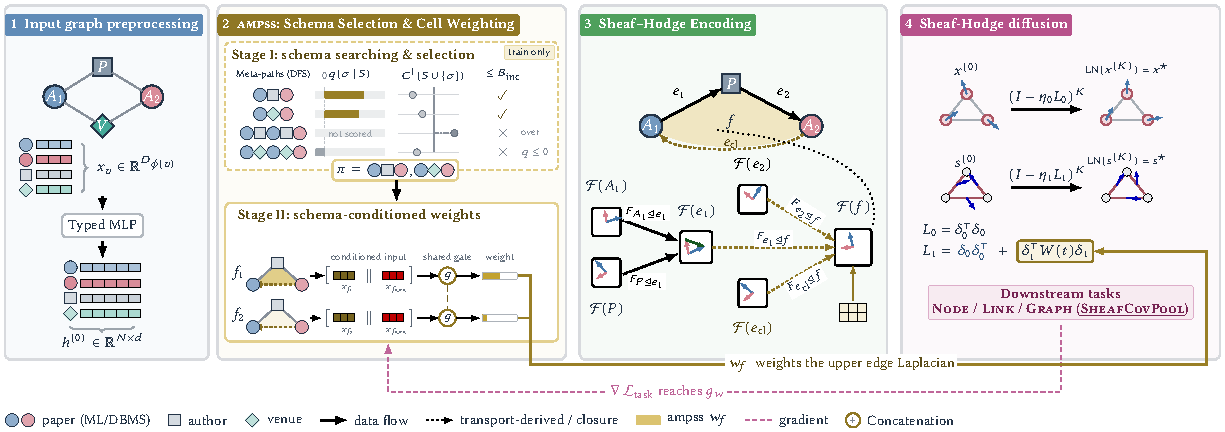
\includegraphics[width=\textwidth]{figure/h2snn_overview.pdf}
  \caption{Overview of \method{} on a citation graph.
\textbf{(1)} Type-specific encoders map heterogeneous node features to a common
\(d\)-dimensional stalk representation.
\textbf{(2)} \ampss{} uses DFS to enumerate meta-path candidates and an auxiliary linear selection model fitted only on the training data to select meta-path schemas in Stage I. In Stage II, it learns schema-conditioned weights for the retained concrete path instances.
\textbf{(3)} Each selected simple path instance is completed by a synthetic
closure \(1\)-cell to form a path-supported \(2D\)-cell. Learned node-to-edge
maps on observed edges define path transports, which construct the closure
restrictions and compatible edge-to-face maps in the corresponding face-stalk
frame.
\textbf{(4)} Node and edge cochains undergo \(K\) parallel Hodge-diffusion steps before task-specific prediction. The learned instance weights modulate the face-induced edge interactions, allowing the supervised task loss to update \ampss{} jointly with the predictor.}
  \Description{A four-panel left-to-right diagram.  Panel one draws a small typed graph and feature
  bars of unequal width becoming bars of equal width d.  Panel two draws a type graph, four
  candidate meta-path schemas with selection-gain bars of which two are kept, and below it two
  concrete path instances of the same schema shaded by their learned weights.  Panel three draws one
  concrete path instance as a shaded polygon closed by a dashed closure edge; below it a node stalk feeds an
  edge stalk, and the stalks of all three boundary edges fan into a single face stalk through
  transports generated by one matrix $A_f$.  Panel four
  draws two parallel diffusion lanes for node and edge cochains and three task heads.  A gold line
  carries the face weight into the upper edge Laplacian and a dashed pink line carries the gradient
  back to the instance-weighting network.}
  \label{fig:pipeline}
\end{figure*}



\subsection{Input Graph Preprocessing: Initialization of Node Stalks and Sheaf Restrictions}

\method{} first maps type-dependent node features into a shared \(d\)-dimensional local feature space (stalk space). This makes representations from different node types compatible with relation-specific restrictions, which transform the endpoint representations into a common edge-stalk space before their disagreement is computed. For each node \(v\), we compute
\begin{equation}
  h_v^{(0)}
  =\operatorname{Dropout}\!\left[
    \operatorname{GELU}\!\left(
      \operatorname{LN}
      \left(W_{\phi(v)}x_v^{\mathrm{raw}}+b_{\phi(v)}\right)
      +q_{\phi(v)}
    \right)
  \right]\in\R^d ,
  \label{eq:node-encoder}
\end{equation}
where \(W_t\) and \(b_t\) are type-specific parameters and \(q_t\) is a learned type embedding. When raw attributes are unavailable, we use a trainable node embedding \(e_v\in\mathbb{R}^{d}\) directly as the initial representation \(h_v^{(0)}\). We initialize the node cochain as \(x^{(0)}=h^{(0)}\) and associate each relation \(r\) with an embedding \(\zeta_r\in\R^{d_r}\).

For an oriented typed edge \(e=(u\xrightarrow{r}v)\), two relation-conditioned networks infer the endpoint restrictions
\(F_{u\unlhd e},F_{v\unlhd e}\in\R^{d\times d}\) from
\(h_u^{(0)}\), \(h_v^{(0)}\), and \(\zeta_r\). The source and target restrictions use the same parameterization:
\begin{equation}
  F_{z\unlhd e}=\lambda_{z,e}Q_{z,e},
  \qquad
  Q_{z,e}^{\transpose}Q_{z,e}=I,
  \qquad
  \lambda_{z,e}>0,
  \quad z\in\{u,v\}.
  \label{eq:conformal-map}
\end{equation}
Here, the orthogonal factor aligns endpoint coordinates, while the positive scale modulates the magnitude of the relation-aware disagreement computed by \(\delta_0\), rather than comparing raw features directly.

We initialize the collection of edge representations (edge cochain) independently from this disagreement:
\begin{equation}
  s_e^{(0)}
  =\operatorname{MLP}_{\mathrm{init}}\!\left(
    h_u^{(0)}\concat h_v^{(0)}\concat \zeta_r
    \concat(\delta_0h^{(0)})_e
  \right).
  \label{eq:edge-init}
\end{equation}
Thus, \(s^{(0)}\) is not restricted to \(\operatorname{im}\delta_0\), allowing the subsequent node-mediated and face-induced edge interactions to act on edge-level information that is not induced solely by node representations. After the selected path instances introduce closure \(1\)-cells, the same coboundary and initialization rules are evaluated over the extended edge set.

\subsection{\ampss{}: Adaptive meta-path schema-to-cell searching and selection}
\label{sec:ampss}

\ampss{} has two stages. Stage I generates candidate meta-path schemas
through bounded depth-first search and selects a task-aligned subset of meta-path schemas from the training data. Stage II assigns schema-conditioned weights to the retained path instances, controlling their contribution to the face-induced edge operator. Thus, Stage I selects typed path patterns, whereas Stage II adapts the influence of individual instances to the
supervised task.

\subsubsection{Stage I: task-aligned schema searching and selection.}
Stage I identifies a compact set of task-relevant meta-path schemas. We
construct a type graph from the relation types available during Stage I and
use bounded depth-first search to generate a candidate pool \(\Pi\) of
schemas \(\pi=(t_0,r_1,t_1,\ldots,r_\ell,t_\ell)\), with lengths between
\(\ell_{\min}\) and \(\ell_{\max}\). Candidates with no feasible simple path
instances are discarded. An edge-face incidence is one occurrence of a boundary edge in a path-supported \(2\)-cell.

For a trial schema set \(S\subseteq\Pi\), deterministic instance and
incidence quotas define the retained instances
\(\mathcal{I}_\pi^q(S)\). These instances provide features derived from the retained path instances of each schema
for an auxiliary linear selection model and determine the structural cost.
Stage I greedily selects schemas subject to a schema limit and instance and
incidence budgets.

The structural cost is the number of retained edge-face incidences:
\begin{equation}
  C^{\mathrm{I}}(S)
  =
  \sum_{\pi\in S}
  \sum_{f\in\mathcal{I}_\pi^q(S)}
  (\ell_f+1),
  \label{eq:stage1-cost}
\end{equation}
%where each path instance contributes \(\ell_f\) path-edge incidences and one
%closure-edge incidence. For graph classification, quotas are applied to each
%training graph and the cost is averaged over the training fold.
where each instance contributes its \(\ell_f\) path edges and one closure edge. Thus, the
incidence budget directly bounds the support of the resulting face-induced edge operator.

The auxiliary linear selection model is fitted on an inner-training
partition and evaluated on a disjoint held-out selection partition. The
gain from adding a candidate schema \(\pi\) is
\begin{equation}
\begin{aligned}
q(\pi \mid S)
&=
\cL_{\mathrm{sel}}(S)
-
\cL_{\mathrm{sel}}(S\cup\{\pi\}),
\qquad
\pi \in \mathcal{A}(S),
\\[3pt]
\mathcal{A}(S)
&=
\left\{
\pi \in \Pi \setminus S
\;\middle|\;
\begin{aligned}
|S\cup\{\pi\}| &\le K_\Sigma,\\
C^{\mathrm{I}}(S\cup\{\pi\}) &\le B_{\mathrm{inc}}
\end{aligned}
\right\}.
\end{aligned}
\label{eq:selection-gain}
\end{equation}
Starting from \(S=\varnothing\), Stage I adds the feasible schema that yields
the largest positive reduction in held-out selection loss. The selection
model is refitted for each trial set using labels from the outer training
split only. For link prediction, inner-selection positive links and their
reverse counterparts are excluded from the graph used for selection. After
selection, the retained instances are constructed on the full outer-training
graph. Because schema selection is discrete, gradients from the \method{}
task loss do not update Stage I. Thus, Stage I provides a task-aligned
schema set for Stage II.

\subsubsection{Stage II: schema-conditioned instance weighting.}
For the schema pool selected in Stage I, Stage II assigns a positive weight
to each retained concrete path instance. Instances sharing the same meta-path
schema can encode different task-relevant information. Let \(\xi_f\) denote
the representation of a retained instance \(f\) produced by the ordered path
encoder before constructing its edge-to-face map \(A_f\), and let
\(e_{\pi(f)}\) denote the embedding of the schema of \(f\). We define
\begin{equation}
  w_f(\tau)
  =
  (1-r(\tau))
  +
  2r(\tau)\,
  \operatorname{sigmoid}\!\left(
    g_w(\xi_f\concat e_{\pi(f)})
  \right),
  \label{eq:instance-weight}
\end{equation}
where \(r(\tau)\in[0,1]\) is a warm-up schedule that gradually changes the weights from uniform to learned values. The output layer of \(g_w\) is
initialized at zero; hence, \(w_f(\tau)=1\) at initialization, and learning
starts from the unweighted face-induced edge interactions. The schema embedding enables
the weighting function to distinguish instances from different schemas, such
as \texttt{PAP} and \texttt{PSP}, whereas \(\xi_f\) distinguishes instances
within the same schema. The weights are learned solely through the supervised
task loss.

Let \(W(\tau)=\mathrm{diag}(w_f(\tau))\). Stage II weights the
face-induced component of the edge operator as
\(\delta_1^{\transpose}W(\tau)\delta_1\). Because \(w_f(\tau)>0\), this
component remains positive semidefinite. The weights therefore modulate only
the contribution of retained path-supported \(2D\)-cells. Closure edges remain
part of the extended edge domain and continue to contribute to
\(\delta_0\), \(L_0\), the node-mediated component of the edge operator, the
weighted face boundary in \(\delta_1\), and the edge readout.

Thus, Stage II provides task-driven, instance-level modulation of the selected path-supported \(2D\)-cells while preserving the extended edge structure.

\subsection{Sheaf-Hodge Encoding}

Because nodes, edges, and selected concrete path instances must be incorporated into the sheaf geometry before they can influence diffusion, we introduce a Sheaf-Hodge encoding to address this requirement. It augments the observed graph with path-supported \(2D\)-cells and defines compatible node-to-edge and edge-to-face restriction maps, preserving the ordered structure of each selected path while enabling node and edge cochains to exchange information through observed relations and retained higher-order supports.

\subsubsection{Augmented Path-Supported \(2\)-Cell Construction}

The Sheaf-Hodge encoder augments the observed graph with retained concrete
path instances. In \ampss{} mode, Stage I selects the corresponding
meta-path schemas and determines the retained instances through its
quotas. Rather than replacing an instance with an endpoint-only relation,
\method{} retains the ordered path and augments it with a synthetic closure \(1\)-cell
\[
  f=(v_0,e_1,v_1,\ldots,e_\ell,v_\ell)
\]
as a path-supported \(2D\)-cell whose boundary preserves the ordered path
edges.

Because this path is open, we introduce a synthetic closure \(1\)-cell,
\(e_{\mathrm{cl}}=(v_\ell\rightarrow v_0)\), to form the closed boundary
\begin{equation}
  \partial f=(e_1,\ldots,e_\ell,e_{\mathrm{cl}}).
  \label{eq:face-boundary}
\end{equation}
The closure \(1\)-cell is not an observed relation, but it is computationally active in the extended edge domain. Its restriction maps are determined by path transport rather than learned independently.

Let \(E_{\mathrm{cl}}\) contain one closure \(1\)-cell for each retained
instance, and let \(E_{\mathrm{ext}}=E\sqcup E_{\mathrm{cl}}\). The retained
instance set is
\[
\mathcal{I}_{\mathrm{ret}}
=
\bigcup_{\pi\in S}\mathcal{I}_\pi^q(S),
\]
where \(S\) denotes the selected schema set. With \(d\)-dimensional node,
edge, and face stalks, the cochain spaces are
\begin{equation}
  C^0(\cF)=\bigoplus_{v\in V}\cF(v),
  \;
  C^1(\cF)=\bigoplus_{e\in E_{\mathrm{ext}}}\cF(e),
  \;
  C^2(\cF)=\bigoplus_{f\in\mathcal{I}_{\mathrm{ret}}}\cF(f).
  \label{eq:extended-cochains}
\end{equation}

After the closure restrictions are defined by the path transport described
below, the first coboundary in Equation~\eqref{eq:prelim-delta0} is evaluated
over \(E_{\mathrm{ext}}\). Hence, closure \(1\)-cells are included in the extended edge domain and
participate in the initial edge cochain and in both \(L_0\) and \(L_1\). We next define the edge-to-face restriction maps for these path-supported \(2D\)-cells in the following section.

\subsubsection{Path-Supported Edge-to-Face Maps}
\label{sec:face-geometry}

The edge-face construction turns each selected concrete path instance into a path-supported \(2D\)-cellular graph. For a selected \(P\!-\!A\!-\!P\) instance, for example, the two paper-author edges remain the boundary
edges of one path-supported \(2D\)-cell.  The intermediate author remains part of the operator through the ordered path boundary, while the synthetic closure edge adds a path-transport-constrained coupling between the endpoints.  This lets the face-induced edge interactions
couple disagreements along the whole paper-author-paper pattern.

For a general instance \(f=(v_0,e_1,v_1,\ldots,e_\ell,v_\ell)\), \method{} first predicts one free
map \(A_f\in\R^{d\times d}\) from the ordered path.  Each face group contains path instances of a single schema, so all instances
in the group have the same length \(\ell\) and relation sequence
\((r_1,\ldots,r_\ell)\).  The default face encoder concatenates the node states in path order
together with the schema's relation embeddings:
\begin{equation}
A_f
=
\operatorname{MLP}_{\ell}\!\left(
  h_{v_0}^{(0)}\concat\cdots\concat h_{v_\ell}^{(0)}
  \concat \zeta_{r_1}\concat\cdots\concat \zeta_{r_\ell}
\right)
\in\mathbb{R}^{d\times d}.
  \label{eq:face-map}
\end{equation}
Here, \(\operatorname{MLP}_{\ell}\) is a path-length-specific MLP that maps
the ordered path representation to the entries of \(A_f\). The resulting map
\(A_f\) defines the local coordinate system of the face stalk for instance
\(f\).
We construct the edge-to-face maps by transporting \(A_f\) along the ordered
path through the node-to-edge restriction maps. This construction ensures
that the face-induced component measures edge-level inconsistency around a
selected path-supported \(2\)-cell, rather than creating an artificial face
signal from an edge cochain induced solely by node representations. Starting
from the base vertex \(v_0\), the transport is
\begin{equation}
  \begin{aligned}
  T_{v_0}&=A_f,
  \qquad
  T_{v_i}=T_{v_{i-1}}F_{u\unlhd e_i}^{-1}F_{v\unlhd e_i},\\
  F_{e_i\unlhd f}&=T_{v_{i-1}}F_{u\unlhd e_i}^{-1},
  \end{aligned}
  \label{eq:transport}
\end{equation}
where \(u=v_{i-1}\) and \(v=v_i\).  

%Because each restriction map is a positive scale times an orthogonal matrix, its inverse has the closed form \(F^{-1}=F^\transpose/\lambda^2\).

The closure edge uses the same path transport:
\begin{equation}
  F_{v_0\unlhd e_{\mathrm{cl}}}=I,
  \qquad
  F_{v_\ell\unlhd e_{\mathrm{cl}}}=T_{v_0}^{-1}T_{v_\ell},
  \qquad
  F_{e_{\mathrm{cl}}\unlhd f}=A_f .
  \label{eq:closure-maps}
\end{equation}
The middle map is the transformation accumulated along the path \(\prod_i F_{u\unlhd e_i}^{-1}F_{v\unlhd e_i}\).  Hence, the closure edge introduces no additional learned restriction map.

Let \(\eta(e,f)\in\{-1,+1\}\) denote the incidence orientation. The weighted second coboundary is
\begin{equation}
  (\delta_{1,w}s)_f
  =
  \sqrt{w_f}
  \sum_{e\in\partial f}
    \eta(e,f)F_{e\unlhd f}s_e .
  \label{eq:delta1}
\end{equation}
Writing
\(B_fs=\sum_{e\in\partial f}\eta(e,f)F_{e\unlhd f}s_e\),
the corresponding face-induced contribution is
\begin{equation}
  \delta_{1,w}^{\transpose}\delta_{1,w}
  =
  \sum_{f\in\mathcal{I}_{\mathrm{ret}}}
    w_f B_f^{\transpose}B_f .
  \label{eq:weighted-up}
\end{equation}

\begin{proposition}[Exact cochain condition]
\label{prop:chain}
For every path instance constructed by \method{} whose node sequence is a
simple path and whose boundary follows the default forward orientation, the
maps in
Eqs.~\eqref{eq:transport} - \eqref{eq:closure-maps} satisfy
\(\delta_{1,w}\delta_0=0\) identically for every node cochain and every value
of the learned parameters.
\end{proposition}
\begin{proof}
By construction \(F_{e_i\unlhd f}F_{u\unlhd e_i}=T_{v_{i-1}}\) and
\(F_{e_i\unlhd f}F_{v\unlhd e_i}=T_{v_i}\).  The \(i\)-th path term of
\(\delta_{1,w}\delta_0x\) is therefore
\(T_{v_i}x_{v_i}-T_{v_{i-1}}x_{v_{i-1}}\), and summing over the path telescopes to
\(T_{v_\ell}x_{v_\ell}-T_{v_0}x_{v_0}\).  The closure maps give
\(F_{e_{\mathrm{cl}}\unlhd f}F_{v_0\unlhd e_{\mathrm{cl}}}=T_{v_0}\) and
\(F_{e_{\mathrm{cl}}\unlhd f}F_{v_\ell\unlhd e_{\mathrm{cl}}}=T_{v_\ell}\), so the closure term
contributes \(T_{v_0}x_{v_0}-T_{v_\ell}x_{v_\ell}\).  The total sum is zero.  The simple-path
condition is required because the transport assigns one map to each node position; a revisited node,
including a coincident endpoint pair, would require two transported values for the same node.
\end{proof}
The chain condition in Proposition~\ref{prop:chain} is scoped to the implemented simple-path,
transport-composed faces and their aligned closure edges.  Within that scope it is
not optimized as an additional penalty but enforced by construction. Its role is to keep
the interpretation of the Hodge decomposition clean: edge signals in \(\operatorname{im}\delta_0\)
come from edge signals induced by node representations, while the face-induced component acts on edge-level residuals around selected
path-supported cycles.

%\begin{figure}[htbp]
%  \centering
%  \fbox{\rule{0pt}{4.2cm}\rule{0.94\columnwidth}{0pt}}
  %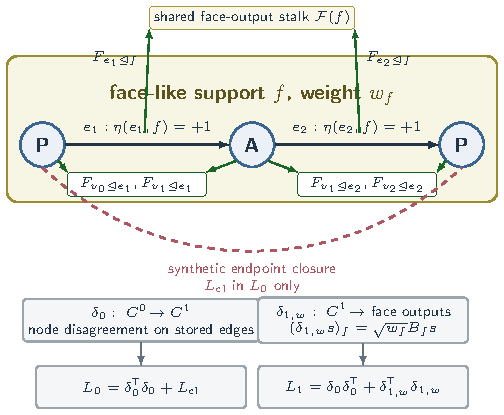
\includegraphics[width=\columnwidth]{figure/h2snn_sheaf_hodge_operator.pdf}
%  \caption{AMPSS-selected path-supported \(2D\)-cells define a sheaf-Hodge operator. Currently in construction.}
%  \label{fig:sheaf-hodge-operator}
%\end{figure}

\subsection{Sheaf-Hodge Diffusion}
\label{sec:closure}

After the restriction maps have been constructed, \method{} diffuses node
and edge cochains using one node operator and one edge operator:
\begin{align}
  L_0x
  &=\delta_0^{\transpose}\delta_0x,
  \label{eq:l0}\\
  L_1s
  &=\underbrace{\delta_0\delta_0^{\transpose}s}_{\text{node-mediated component}}
    +\underbrace{\delta_{1,w}^{\transpose}\delta_{1,w}s}_{\text{face-induced component}} .
  \label{eq:l1}
\end{align}
The node operator \(L_0\) compares transported endpoint signals. The edge diffusion operator \(L_1\) contains a node-mediated component and a face-induced component. The
node-mediated component of \(L_1\) relates edge signals through shared
incident nodes, whereas the face-induced component couples boundary edges
within selected path-supported \(2D\)-cells. In Hodge-theoretic terminology,
these are the lower and upper components of the edge operator, which represent node-mediated and face-induced edge interactions, respectively. Because each closure \(1\)-cell is part of the extended edge
set, it participates in both components without requiring a separate
node-side correction.

Starting from \(x^{(0)}=h^{(0)}\) and the independently initialized edge cochain \(s^{(0)}\),
\(K\) explicit Euler steps give
\begin{equation}
  \begin{aligned}
  x^{(k+1)}&=x^{(k)}-\alpha_0L_0x^{(k)},\\
  s^{(k+1)}&=s^{(k)}-\alpha_1L_1s^{(k)},
  \qquad k=0,\ldots,K-1 .
  \end{aligned}
  \label{eq:diffusion}
\end{equation}
The positive step sizes may be learned.  Node and edge cochains are updated by separate \(L_0\) and \(L_1\) operators. Although updated node and edge states are not exchanged between diffusion steps, both operators share the learned restriction geometry and initial node representations. Layer normalization then gives the terminal states \(x^\star\) and \(s^\star\), which are passed to
the task-specific readout.

The Hodge operators are evaluated through local restriction maps and indexed aggregation without explicitly forming global operators. The implementation batches local restriction maps and aggregates
contributions with indexed sums.  This applies \(\delta_0\), \(\delta_0^{\transpose}\),
\(\delta_{1,w}\), and \(\delta_{1,w}^{\transpose}\) directly on node, edge, and face tensors.

Three implementation boundaries are important.  First, \(\delta_{1,w}\) uses the complete boundary
cycle, consisting of the \(\ell\) path edges and the closure \(1\)-cell.  Second, incidence signs are
represented explicitly.  The paths produced by the current enumeration use \(+1\) signs because the enumeration follows stored edge directions and orients the closure edge along the cycle.  Third, the exact
transport argument assumes simple paths, so instances that revisit a node, including coincident
endpoints, are excluded during enumeration.  Under these constraints, the chain condition is a
property of the constructed operator, not a penalty added to the training objective.

The shared backbone produces final node states \(x^\star\) and edge states \(s^\star\). For node classification, the target-node state is combined with pooled incident-edge information. For link prediction, endpoint representations are formed from node and incident-edge states before applying a pair decoder. For graph classification, \sheafcovpool{} aggregates node and edge
representations into a graph-level vector, as described next.

\subsection{\sheafcovpool{}}

Graph classification requires one representation for the whole graph, yet node and edge states
are expressed in different local coordinate systems. Averaging incident edge coordinates directly
would therefore mix vectors from different spaces. Before pooling, \sheafcovpool{} projects each incident edge state into the corresponding node coordinate space using the transpose of its restriction map:
\begin{equation}
  \widetilde{s}_v^\star
  =
  \frac{1}{\deg_{\mathrm{ext}}(v)}
  \left(
  \sum_{e:\operatorname{src}(e)=v}
  F_{\mathrm{src},e}^{\transpose}s_e^\star
  +
  \sum_{e:\operatorname{tgt}(e)=v}
  F_{\mathrm{tgt},e}^{\transpose}s_e^\star
  \right).
  \label{eq:pool-transport}
\end{equation}
Here \(F_{\mathrm{src},e}\) and \(F_{\mathrm{tgt},e}\) denote the restriction maps from the source
and target nodes of \(e\), respectively, into the edge stalk. \(\deg_{\mathrm{ext}}(v)\) is the
number of incidences at \(v\) over observed and closure edges; an isolated node receives the zero vector.
Both endpoints contribute positively because this quantity summarizes incident context rather than
the orientation-sensitive divergence \(\delta_0^{\transpose}s^\star\). The sums range over the
observed and closure edges, so both types of \(1\)-cell contribute.

The readout then forms three complementary views at each node and edge:
\begin{equation}
  \begin{aligned}
  Z_v^{(0)}
  &=\begin{bmatrix}x_v^\star&h_v^{(0)}&\widetilde{s}_v^\star\end{bmatrix}
    \in\R^{d\times3},\\
  Z_e^{(1)}
  &=\begin{bmatrix}
    (\delta_0x^\star)_e&(\delta_0h^{(0)})_e&s_e^\star
  \end{bmatrix}
    \in\R^{d\times3},\\
   G_i^{(q)}
   &=(Z_i^{(q)})^{\transpose}Z_i^{(q)}
     \in\R^{3\times3},\qquad q\in\{0,1\}.
  \end{aligned}
  \label{eq:pool-views}
\end{equation}
This matrix records the energies and pairwise alignments of the three views while removing their
common orthogonal orientation; we call it a Gram matrix. For an ordered view stack, equality of Gram matrices
characterizes equality up to an orthogonal change of basis.

To see why the transported node view has this property, let \(Q_v,R_e\in O(d)\) be independent
changes of basis in the node and edge stalks. Under the consistent transformation
\begin{equation}
  \begin{aligned}
  F_{v\unlhd e}'&=R_eF_{v\unlhd e}Q_v^{\transpose},
  \qquad s_e^{\star\prime}=R_es_e^\star,\\
  (F_{v\unlhd e}')^{\transpose}s_e^{\star\prime}
  &=Q_vF_{v\unlhd e}^{\transpose}s_e^\star .
  \end{aligned}
  \label{eq:pool-gauge}
\end{equation}
Hence \(Z_v^{(0)}\) transforms by \(Q_v\), while \(Z_e^{(1)}\) transforms by \(R_e\), and both Gram
descriptors remain unchanged. This argument requires orthogonal basis changes; the learned
restrictions themselves may be scaled orthogonal maps.

Nodes and edges serve different roles, so separate networks project their Gram matrices.
Within graph \(g\), attention over these invariant descriptors yields first- and second-order
summaries:
\begin{equation}
  \begin{aligned}
   u_i^{(q)}&=\rho_q(\operatorname{vec}G_i^{(q)})\in\R^{F},\\
   a_i^{(q)}
   &=\frac{\exp(g_q(u_i^{(q)}))}
           {\sum_{j\in\mathcal{C}_q(g)}\exp(g_q(u_j^{(q)}))},\\
   \mu_q(g)&=\sum_{i\in\mathcal{C}_q(g)}a_i^{(q)}u_i^{(q)},\\
   \Sigma_q(g)&=\sum_{i\in\mathcal{C}_q(g)}a_i^{(q)}
     (u_i^{(q)}-\mu_q(g))(u_i^{(q)}-\mu_q(g))^{\transpose}.
  \end{aligned}
  \label{eq:pool-moments}
\end{equation}
Here \(q\in\{0,1\}\), \(\mathcal{C}_0(g)\) is the node set, and \(\mathcal{C}_1(g)\) contains the observed and closure
edges. The mean describes the evidence emphasized by attention, whereas the covariance
records how that evidence varies across the graph. The final graph representation is
\begin{equation}
  \gamma_g=
  \bigl[
  \mu_0(g)\concat\operatorname{triu}(\Sigma_0(g))
  \concat\mu_1(g)\concat\operatorname{triu}(\Sigma_1(g))
  \bigr].
  \label{eq:pool-summary}
\end{equation}
The order of the raw Gram matrix is fixed at three because it is determined by the three
semantic views in each stack, rather than by a freely chosen hidden width. Changing that order
would require adding or removing stalk-valued views and would therefore define a different readout.
We instead control readout capacity through the post-Gram projection width \(F\). The two means and
two upper-triangular covariance vectors give \(\gamma_g\in\R^{F^2+3F}\).
Because every learned score acts on an invariant Gram matrix and every aggregation is
symmetric, \(\gamma_g\) is invariant to node and edge ordering. Given consistently transformed
states and restriction maps, it is also invariant to independent orthogonal changes of basis in
the node and edge stalks.

\begin{figure}[htbp]
  \centering
  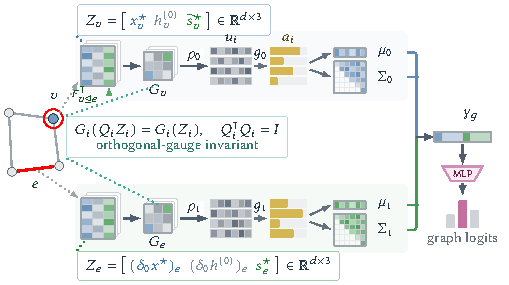
\includegraphics[width=\columnwidth]{figure/sheafcovpool_architecture.pdf}
  \caption{\sheafcovpool{} graph readout. Incident edge states are first expressed in their endpoint node stalks. Node and edge view stacks then become gauge-invariant Gram matrices \(G_i\); attention-weighted means and covariances form the graph representation \(\gamma_g\).}
  \Description{Two parallel lanes, node above and edge below, both fed by the same small graph on
  the left in which every node and edge carries its own local basis.  In each lane a stack of
  three stalk-valued views becomes a three-by-three Gram matrix, a learned projection turns it into
  a token, a learned score turns tokens into attention weights that sum to one within the graph,
  and those weights produce a weighted mean vector and a weighted covariance matrix whose upper
  triangle is kept.  The four summaries concatenate into one vector that an MLP maps to graph
  logits.}
  \label{fig:sheafcovpool}
\end{figure}



\section{Experiments}
\label{sec:experiments}

\subsection{Experiment Settings}
\label{sec:experiment-settings}
To assess the generalizability of \method{} across heterogeneous graph learning settings, we evaluated it on three tasks: node classification, link prediction, and graph classification.
\paragraph{Datasets.}
For node classification, we used three heterogeneous graph benchmarks: DBLP and IMDB from HGB \cite{lv2021hgb} and ACM \cite{wang2019han}. For graph classification, we selected four datasets from TUDataset \cite{morris2020tudataset}: two biological datasets, PROTEINS and ENZYMES, and two chemical-compound datasets, MUTAG and NCI1. To make the graph heterogeneous, we interpreted the node and edge labels provided by TUDataset as node and relation types, respectively. For link prediction, we used four HGB benchmarks \cite{lv2021hgb}: three user-item interaction networks, LastFM, YouTube, and Amazon, and one biological knowledge graph, PubMed. Dataset statistics are reported in Tables~\ref{tab:node-cls}, \ref{tab:graph-cls}, and~\ref{tab:link-pred}.

\paragraph{Baselines.}
For node classification, we compared \method{} with baselines from four model categories. The homogeneous homophilic baselines comprised GCN \cite{kipf2017gcn}, GAT \cite{velickovic2018gat}, and ChebNetII \cite{he2022chebnetii}, while the homogeneous heterophilic baselines included NSD \cite{bodnar2022neural} and CSNN \cite{ribeiro2026cooperative}. For heterogeneous graphs, we considered the homophilic models HAN \cite{wang2019han}, SeHGNN \cite{yang2023sehgnn}, HiNormer \cite{mao2023hinormer}, and PSHGCN \cite{he2024spectral}, as well as the heterophilic models HDHGR \cite{guo2023homophily}, Hetero$^2$Net \cite{li2025hetero2net}, H2SGNN \cite{lu2026addressing}, HetSheaf \cite{braithwaite2024heterogeneous}, and LatGRL \cite{shen2025heterophily}.
For graph classification and link prediction, we used a subset of these baselines while retaining representatives from all four categories. Specifically, we included GCN \cite{kipf2017gcn} and GAT \cite{velickovic2018gat} as homogeneous homophilic models; NSD \cite{bodnar2022neural} and CSNN \cite{ribeiro2026cooperative} as homogeneous heterophilic models; HAN \cite{wang2019han} and PSHGCN \cite{he2024spectral} as heterogeneous homophilic models; and HDHGR \cite{guo2023homophily}, Hetero$^2$Net \cite{li2025hetero2net}, H2SGNN \cite{lu2026addressing}, HetSheaf \cite{braithwaite2024heterogeneous}, and LatGRL \cite{shen2025heterophily} as heterogeneous heterophilic models.
\paragraph{Evaluation Settings.}
For node classification, we followed the HGB benchmark protocol \cite{lv2021hgb}, using transductive training/validation/test splits of 20\%/20\%/60\% and reporting Macro-F1 and Micro-F1. For graph classification, following prior work \cite{zhang2018end,amouzad2024graphunet}, we performed 10-fold cross-validation over five random seeds and reported the mean and standard deviation of Macro-F1 and Micro-F1. For the multi-class ENZYMES dataset, we adopted a one-vs-rest strategy. For link prediction, we followed the HGB protocol \cite{lv2021hgb}, using transductive splits of 81\%/9\%/10\% and reporting AUPR and AUROC. Negative edges were sampled from the 2-hop neighborhood at a 1:1 ratio to positive edges. All models were trained with early stopping using a patience of 100 epochs. Hyperparameters were selected through per-dataset sweeps, with the complete configurations provided in Appendix~\ref{app:hyperparameters}. We group the baselines according to graph type and homophily assumption as Hom./hom., Hom./het., Het./hom., and Het./het., where the first term indicates whether the graph is modeled as homogeneous or heterogeneous and the second indicates whether the method is designed for homophilic or heterophilic settings. Results are averaged over five random seeds and reported with standard deviations. The code is available at \url{placeholder_for_code_repository.com}.
\subsection{Results}
\label{sec:results}

For the node-classification tasks, the results in Table~\ref{tab:node-cls} show that \method{} achieved the best performance on all three benchmark datasets, outperforming every compared baseline. This demonstrates the effectiveness of \method{} in capturing complex heterogeneous graph structures and relationships, leading to improved node classification performance.

\begin{table*}[htbp]
  \centering
  \caption{Performance on node classification benchmarks measured by Macro-F1 and Micro-F1. Best values are bold.}
  \label{tab:node-cls}
  \scriptsize
  \resizebox{0.8\textwidth}{!}{%
  \begin{tabular}{llcccccc}
    \toprule
    & &
    \multicolumn{2}{c}{DBLP (59.76)} &
    \multicolumn{2}{c}{ACM (72.39)} &
    \multicolumn{2}{c}{IMDB (50.04)} \\
    \cmidrule(lr){3-4}
    \cmidrule(lr){5-6}
    \cmidrule(lr){7-8}
    \textbf{Group} & \textbf{Model}
    & Macro-F1 & Micro-F1
    & Macro-F1 & Micro-F1
    & Macro-F1 & Micro-F1 \\
    \midrule

    \multirow{3}{*}{Hom./hom.}
    & GCN
    & $90.77 \pm 0.76$
    & $90.28 \pm 0.20$
    & $91.63 \pm 0.44$
    & $91.38 \pm 0.39$
    & $62.33 \pm 0.58$
    & $67.69 \pm 0.59$ \\

    & GAT
    & $94.39 \pm 1.03$
    & $92.52 \pm 0.27$
    & $92.07 \pm 0.57$
    & $90.71 \pm 0.21$
    & $62.13 \pm 0.26$
    & $68.09 \pm 0.48$ \\
    
    & ChebNetII
    & $92.89 \pm 1.07$
    & $92.67 \pm 0.50$
    & $91.70 \pm 0.27$
    & $91.59 \pm 0.27$
    & $62.97 \pm 0.66$
    & $68.47 \pm 0.55$ \\

    \midrule

    \multirow{2}{*}{Hom./het.}
    & NSD
    & $92.96 \pm 0.21$
    & $93.42 \pm 0.37$
    & $92.33 \pm 0.78$
    & $92.05 \pm 0.69$
    & $61.61 \pm 0.26$
    & $65.23 \pm 0.51$ \\


    & CSNN
    & $93.73 \pm 0.95$
    & $92.12 \pm 0.19$
    & $93.13 \pm 0.94$
    & $92.81 \pm 0.83$
    & $62.92 \pm 0.34$
    & $62.59 \pm 0.22$ \\


    \midrule

    \multirow{4}{*}{Het./hom.}
    & HAN
    & $91.78 \pm 0.92$
    & $92.24 \pm 0.86$
    & $90.88 \pm 0.67$
    & $91.61 \pm 1.07$
    & $61.95 \pm 0.36$
    & $67.76 \pm 0.51$ \\

    & SeHGNN
    & $95.52 \pm 0.98$
    & $95.48 \pm 0.78$
    & $94.38 \pm 1.00$
    & $94.04 \pm 0.73$
    & $72.01 \pm 0.65$
    & $72.59 \pm 0.18$ \\

    & HiNormer
    & $94.06 \pm 0.40$
    & $94.14 \pm 0.46$
    & $91.87 \pm 0.26$
    & $89.64 \pm 0.39$
    & $64.13 \pm 0.19$
    & $67.53 \pm 0.32$ \\

    & PSHGCN
    & $95.58 \pm 0.80$
    & $95.70 \pm 0.54$
    & $93.66 \pm 0.53$
    & $94.70 \pm 0.39$
    & $71.82 \pm 0.34$
    & $74.34 \pm 0.84$ \\
    \midrule

    \multirow{5}{*}{Het./het.}
    & HDHGR
    & $95.35 \pm 0.81$
    & $95.00 \pm 0.77$
    & $93.99 \pm 0.35$
    & $94.13 \pm 0.87$
    & $59.41 \pm 0.22$
    & $59.63 \pm 0.35$ \\

    & Hetero$^2$Net
    & $93.54 \pm 1.11$
    & $93.54 \pm 0.79$
    & $94.05 \pm 0.71$
    & $92.87 \pm 0.82$
    & $65.34 \pm 0.68$
    & $70.63 \pm 0.69$ \\

    & H2SGNN
    & $95.82 \pm 0.41$
    & $95.11 \pm 0.22$
    & $94.90 \pm 0.49$
    & $94.08 \pm 0.44$
    & $74.23 \pm 0.31$
    & $75.29 \pm 0.86$ \\

    & HetSheaf
    & $93.87 \pm 0.00$
    & $93.77 \pm 0.00$
    & $95.09 \pm 0.00$
    & $94.94 \pm 0.00$
    & $64.65 \pm 0.00$
    & $67.18 \pm 0.00$ \\

    & LatGRL
    & $94.32 \pm 0.44$
    & $94.51 \pm 0.42$
    & $93.47 \pm 0.71$
    & $92.29 \pm 0.43$
    & $58.27 \pm 0.46$
    & $58.81 \pm 0.65$ \\
    \midrule

    Ours
    & \textbf{\method{}}
    & $\mathbf{96.01 \pm 0.58}$
    & $\mathbf{96.31 \pm 0.40}$
    & $\mathbf{95.91 \pm 1.15}$
    & $\mathbf{95.72 \pm 0.68}$
    & $\mathbf{75.05 \pm 0.22}$
    & $\mathbf{76.68 \pm 0.19}$ \\
    \bottomrule
  \end{tabular}%
  }
\end{table*}

Moreover, for the graph classification tasks, table~\ref{tab:graph-cls} shows that \method{} tied the best reported MUTAG score and achieved the highest mean Macro-F1 and Micro-F1 on PROTEINS, ENZYMES, and NCI1 among the compared baselines. This suggests that treating the typed node and edge labels as heterogeneous structure, rather than as plain homogeneous graphs with categorical attributes, remains useful even outside the citation- and social-network domains where heterogeneity is usually studied.

\begin{table*}[htbp]
  \centering
  \caption{Performance on graph classification benchmarks measured by Macro-F1 and Micro-F1. Best values are bold.}
  \label{tab:graph-cls}
  \scriptsize
  \resizebox{0.8\textwidth}{!}{%
  \begin{tabular}{llcccccccc}
    \toprule
    & &
    \multicolumn{2}{c}{MUTAG} &
    \multicolumn{2}{c}{PROTEINS} &
    \multicolumn{2}{c}{ENZYMES} &
    \multicolumn{2}{c}{NCI1} \\
    \cmidrule(lr){3-4}
    \cmidrule(lr){5-6}
    \cmidrule(lr){7-8}
    \cmidrule(lr){9-10}
    \textbf{Group} & \textbf{Model}
    & Macro-F1 & Micro-F1
    & Macro-F1 & Micro-F1
    & Macro-F1 & Micro-F1
    & Macro-F1 & Micro-F1 \\
    \midrule

    \multirow{2}{*}{Hom./hom.}
    & GCN
    & $89.58 \pm 0.63$
    & $90.00 \pm 0.38$
    & $75.92 \pm 0.55$
    & $79.83 \pm 0.49$
    & $12.75 \pm 0.01$
    & $28.33 \pm 0.03$
    & $64.17 \pm 0.29$
    & $64.96 \pm 0.38$ \\

    & GAT
    & $89.58 \pm 0.06$
    & $90.00 \pm 0.96$
    & $75.27 \pm 0.59$
    & $78.38 \pm 0.71$
    & $14.03 \pm 0.05$
    & $16.55 \pm 0.12$
    & $64.17 \pm 0.27$
    & $64.96 \pm 0.69$ \\
    \midrule

    \multirow{2}{*}{Hom./het.}
    & NSD
    & $\mathbf{99.47 \pm 0.53}$
    & $\mathbf{99.69 \pm 0.31}$
    & $73.60 \pm 0.22$
    & $75.89 \pm 0.49$
    & $33.65 \pm 0.37$
    & $35.00 \pm 0.21$
    & $72.30 \pm 0.31$
    & $72.30 \pm 0.10$ \\

    & CSNN
    & $\mathbf{99.21 \pm 0.79}$
    & $\mathbf{99.40 \pm 0.60}$
    & $76.64 \pm 0.28$
    & $77.92 \pm 0.07$
    & $35.15 \pm 0.07$
    & $37.22 \pm 0.13$
    & $74.11 \pm 0.75$
    & $74.30 \pm 0.80$ \\
    \midrule

    \multirow{2}{*}{Het./hom.}
    & HAN
    & $82.91 \pm 0.61$
    & $85.00 \pm 0.19$
    & $79.19 \pm 0.82$
    & $82.22 \pm 0.50$
    & $46.24 \pm 0.06$
    & $45.02 \pm 0.06$
    & $77.60 \pm 0.43$
    & $77.50 \pm 0.29$ \\

    & PSHGCN
    & $94.88 \pm 0.10$
    & $95.00 \pm 0.42$
    & $70.61 \pm 0.13$
    & $72.32 \pm 0.74$
    & $60.18 \pm 0.24$
    & $58.33 \pm 0.38$
    & $74.17 \pm 0.34$
    & $74.96 \pm 0.37$ \\
    \midrule

    \multirow{5}{*}{Het./het.}
    & HDHGR
    & $84.65 \pm 0.71$
    & $85.00 \pm 0.64$
    & $77.64 \pm 0.83$
    & $81.25 \pm 0.65$
    & $58.27 \pm 0.21$
    & $58.33 \pm 0.64$
    & $79.29 \pm 0.61$
    & $79.32 \pm 0.18$ \\

    & Hetero$^2$Net
    & $89.58 \pm 0.16$
    & $90.00 \pm 0.62$
    & $74.66 \pm 0.69$
    & $78.57 \pm 0.43$
    & $61.53 \pm 0.21$
    & $61.36 \pm 0.49$
    & $63.67 \pm 0.66$
    & $65.45 \pm 0.38$ \\

    & H2SGNN
    & $94.88 \pm 0.09$
    & $95.00 \pm 0.35$
    & $70.61 \pm 0.37$
    & $72.32 \pm 0.14$
    & $62.18 \pm 0.44$
    & $61.31 \pm 0.45$
    & $64.17 \pm 0.06$
    & $64.96 \pm 0.44$ \\

    & HetSheaf
    & $\mathbf{100.00 \pm 0.00}$
    & $\mathbf{100.00 \pm 0.00}$
    & $80.56 \pm 0.00$
    & $82.14 \pm 0.00$
    & $62.35 \pm 0.00$
    & $63.33 \pm 0.00$
    & $79.46 \pm 0.00$
    & $79.46 \pm 0.00$ \\

    & LatGRL
    & $90.88 \pm 0.99$
    & $91.01 \pm 0.11$
    & $71.61 \pm 0.20$
    & $72.32 \pm 0.33$
    & $60.41 \pm 0.09$
    & $60.03 \pm 0.39$
    & $77.98 \pm 0.11$
    & $78.10 \pm 0.41$ \\
    \midrule

    Ours
    & \textbf{\method{}}
    & $\mathbf{99.65 \pm 0.35}$
    & $\mathbf{99.72 \pm 0.28}$
    & $\mathbf{84.44 \pm 0.21}$
    & $\mathbf{86.23 \pm 0.15}$
    & $\mathbf{64.52 \pm 0.56}$
    & $\mathbf{65.10 \pm 0.37}$
    & $\mathbf{81.22 \pm 0.06}$
    & $\mathbf{81.52 \pm 0.20}$ \\
    \bottomrule
  \end{tabular}%
  }
\end{table*}

The link-prediction results in Table~\ref{tab:link-pred} show that \method{} achieves the best performance on all four link-prediction datasets and all eight reported metrics. This advantage is consistent across multi-node-type graphs (LastFM and
PubMed) and single-node-type, multi-relation graphs (Amazon and YouTube). These results indicate that \method{} supports link prediction on both multi-node-type graphs and single-node-type, multi-relation graphs.

\begin{table*}[htbp]
  \centering
  \caption{Performance on link prediction benchmarks measured by AUPR and AUROC. Best values are bold.}
  \label{tab:link-pred}
  \scriptsize
  \setlength{\tabcolsep}{2.5pt}
  \resizebox{0.8\textwidth}{!}
  {%
  \begin{tabular}{llcccccccc}
    \toprule
    & & \multicolumn{2}{c}{LastFM} & \multicolumn{2}{c}{PubMed} & \multicolumn{2}{c}{Amazon} & \multicolumn{2}{c}{YouTube} \\
    \cmidrule(lr){3-4}\cmidrule(lr){5-6}\cmidrule(lr){7-8}\cmidrule(lr){9-10}
    \textbf{Group} & \textbf{Model} & AUPR & AUROC & AUPR & AUROC & AUPR & AUROC & AUPR & AUROC \\
    \midrule

    \multirow{2}{*}{Hom./hom.}
    & GCN
    & $97.06 \pm 0.48$ & $96.96 \pm 0.41$
    & $96.05 \pm 0.52$ & $92.93 \pm 0.36$
    & $92.40 \pm 0.61$ & $89.66 \pm 0.73$
    & $89.30 \pm 0.39$ & $83.26 \pm 0.52$ \\
    & GAT
    & $63.06 \pm 0.27$ & $51.14 \pm 0.19$
    & $96.07 \pm 0.43$ & $93.27 \pm 0.68$
    & $88.62 \pm 0.34$ & $86.10 \pm 0.45$
    & $66.76 \pm 0.31$ & $58.40 \pm 0.22$ \\
    \midrule

    \multirow{2}{*}{Hom./het.}
    & NSD
    & $97.16 \pm 0.71$ & $96.58 \pm 0.65$
    & $96.41 \pm 0.58$ & $93.65 \pm 0.74$
    & $92.63 \pm 0.49$ & $90.04 \pm 0.38$
    & $89.32 \pm 0.43$ & $83.36 \pm 0.57$ \\
    & CSNN
    & $97.99 \pm 0.42$ & $97.75 \pm 0.39$
    & $96.14 \pm 0.30$ & $92.87 \pm 0.29$
    & $92.10 \pm 0.53$ & $89.62 \pm 0.41$
    & $88.64 \pm 0.34$ & $82.97 \pm 0.48$ \\
    \midrule

    \multirow{2}{*}{Het./hom.}
    & HAN
    & $88.26 \pm 0.37$ & $83.32 \pm 0.46$
    & $95.78 \pm 0.49$ & $93.62 \pm 0.62$
    & $95.24 \pm 0.56$ & $93.64 \pm 0.60$
    & $92.46 \pm 0.51$ & $90.10 \pm 0.42$ \\
    & PSHGCN
    & $88.02 \pm 0.44$ & $80.55 \pm 0.50$
    & $97.58 \pm 0.35$ & $93.27 \pm 0.68$
    & $94.28 \pm 0.46$ & $92.34 \pm 0.42$
    & $93.15 \pm 0.63$ & $90.66 \pm 0.58$ \\
    \midrule

    \multirow{5}{*}{Het./het.}
    & HDHGR
    & $97.89 \pm 0.51$ & $97.93 \pm 0.45$
    & $95.03 \pm 0.77$ & $93.15 \pm 0.36$
    & $93.37 \pm 0.40$ & $91.42 \pm 0.59$
    & $91.68 \pm 0.65$ & $88.33 \pm 0.38$ \\
    & Hetero$^2$Net
    & $97.58 \pm 0.29$ & $97.45 \pm 0.61$
    & $94.66 \pm 0.53$ & $92.57 \pm 0.47$
    & $94.71 \pm 0.54$ & $92.34 \pm 0.42$
    & $90.67 \pm 0.70$ & $86.45 \pm 0.41$ \\
    & H2SGNN
    & $97.88 \pm 0.36$ & $97.22 \pm 0.68$
    & $95.22 \pm 0.42$ & $92.32 \pm 0.55$
    & $93.18 \pm 0.61$ & $92.31 \pm 0.50$
    & $90.17 \pm 0.46$ & $88.96 \pm 0.64$ \\
    & LatGRL
    & $96.88 \pm 0.62$ & $96.01 \pm 0.71$
    & $96.61 \pm 0.48$ & $92.32 \pm 0.52$
    & $94.41 \pm 0.43$ & $92.03 \pm 0.57$
    & $89.98 \pm 0.35$ & $88.10 \pm 0.49$ \\
    & HetSheaf
    & $98.51 \pm 0.00$ & $98.00 \pm 0.00$
    & $96.36 \pm 0.00$ & $93.00 \pm 0.00$
    & $93.76 \pm 0.00$ & $91.00 \pm 0.00$
    & $91.27 \pm 0.00$ & $88.00 \pm 0.00$ \\
    \midrule

    Ours
    & \textbf{\method{}}
    & $\mathbf{98.91 \pm 0.37}$ & $\mathbf{98.72 \pm 0.35}$
    & $\mathbf{97.63 \pm 0.41}$ & $\mathbf{96.48 \pm 0.54}$ 
    & $\mathbf{98.53 \pm 0.56}$ & $\mathbf{98.33 \pm 0.44}$
    & $\mathbf{93.95 \pm 0.47}$ & $\mathbf{91.81 \pm 0.33}$  \\
    \bottomrule
  \end{tabular}%
  }
\end{table*}

\section{Discussion}
\label{sec:analysis-results}

\subsection{Ablation Study: Contribution of {\ampss{}}}

To evaluate \ampss{}, we compared the full \method{} on DBLP node classification with variants using no path-supported \(2D\)-cells, predefined meta-path schemas, \ampss{} with Stage-I selection only, and Stage-II weighting without the instance gate. As shown in Table~\ref{tab:ablation-schema}, removing path-supported \(2D\)-cells decreased Macro-F1/Micro-F1, confirming that path-supported \(2D\)-cells contribute to node classification. Predefined meta-path schemas recovered most of this loss, while the full \ampss{} model performed best. These results suggest that automatic meta-path schema selection can improve performance, but schema-level selection alone is insufficient; instance-level weighting helps filter noisy or uninformative path realizations.

\begin{table}[H]
  \centering
  \caption{Ablation Study of \ampss{} on DBLP node classification.}
  \label{tab:ablation-schema}
  \small
  \begin{tabular}{lcc}
    \toprule
    \textbf{Configuration} & Macro-F1 & Micro-F1 \\
    \midrule
    No path-supported \(2D\)-cells & 93.85 & 93.92 \\
    Predefined meta-path schemas & 95.75 & 96.01 \\
    \ampss{}, stage I only & 95.88 & 96.02 \\
    \ampss{}, schema weight only & 95.91 & 96.08 \\
    \ampss{}, instance weight only & 95.95 & 96.13 \\
    \textbf{\ampss{}} & \textbf{96.01} & \textbf{96.31} \\
    \bottomrule
  \end{tabular}
\end{table}

\subsection{Ablation Study: Contribution of {\sheafcovpool{}}}

To evaluate \sheafcovpool{}, we compared the full \method{} on ENZYMES graph classification with sum, mean, and max pooling, SheafPool~\cite{braithwaite2024heterogeneous}, and \sheafcovpool{}. As shown in Table~\ref{tab:ablation-pooling}, SheafPool improved Macro-F1/Micro-F1 to \(64.05/64.96\), indicating that, under this protocol, a gauge-invariant readout retained information not captured by the three plain aggregation baselines. \sheafcovpool{} performed best because \sheafcovpool{} pools both node and edge Gram matrices and retains attention-weighted means together with across-node and across-edge covariances. These results suggest that gauge invariance is useful but not sufficient, and that retaining second-order statistics of the node and edge cochains is important for graph-level prediction.
\begin{table}[H]
  \centering
  \caption{Ablation study of graph-level readouts on ENZYMES graph classification.}
  \label{tab:ablation-pooling}
  \small
  \begin{tabular}{lcc}
    \toprule
    \textbf{Readout} & Macro-F1 & Micro-F1 \\
    \midrule
    Sum + MLP & 61.25 & 61.79 \\
    Mean + MLP & 61.42 & 62.09 \\
    Max + MLP & 61.38 & 61.62 \\
    SheafPool & 64.05 & 64.96 \\
    \textbf{\sheafcovpool{}} & \textbf{64.52} & \textbf{65.10} \\
    \bottomrule
  \end{tabular}
\end{table}

\section{Conclusion}
To address heterogeneous graph learning under heterophily, We presented \method{}, a heterogeneous heterophilic sheaf neural network for supervised learning on typed graphs. The model retains selected concrete meta-path instances as path-supported \(2D\)-cells rather than collapsing them into endpoint-level views. Learned restriction maps and sheaf-Hodge diffusion jointly update node and edge cochains, allowing these ordered path structures to influence propagation. \ampss{} selects task-relevant schemas and learns schema-conditioned weights for retained path instances, while \sheafcovpool{} provides a permutation- and gauge-invariant graph-level readout that combines node and incident-edge information.
On the evaluated benchmarks, \method{} achieved the best results on all node-classification, graph-classification, and link-prediction datasets. The ablations support the contributions of \ampss{} and \sheafcovpool{}. These results suggest that retaining typed, ordered path structure and learning sheaf-based propagation can provide a useful framework for heterogeneous heterophilic graph learning.


\bibliographystyle{ACM-Reference-Format}
\bibliography{references}

\appendix

\section{Data Preparation}
\label{sec:data-prep}

\subsection{Downstream Readouts}
\label{sec:readouts}

After sheaf-Hodge diffusion, the model has integrated information across both nodes and
typed relations while retaining representations at the node and edge levels.  Different
prediction tasks, however, require this information to be summarized differently: node
classification is centered on an individual target node, whereas link and graph prediction
also depend on relational or graph-level structure.  We therefore keep the sheaf-Hodge
backbone shared across tasks and use a lightweight task-specific readout to convert the
relevant final representations into logits.

Specifically, the backbone produces final node states \(x^\star\), final edge states
\(s^\star\), and the initial typed node states \(h^{(0)}\), which the corresponding decoder
uses according to the downstream task.

\paragraph{Node classification.}
For node classification, the readout pools the states of observed and closure edges incident to
each target node \(v\in V_{\mathrm{target}}\), where \(V_{\mathrm{target}}\subseteq V\) denotes the
target-node set. Let \(E(v)\) denote this set of incident edges:
\begin{equation}
  \bar s_v^\star
  =
  \begin{cases}
    |E(v)|^{-1}\sum_{e\in E(v)}s_e^\star, & |E(v)|>0,\\
    0, & |E(v)|=0 ,
  \end{cases}
  \label{eq:node-edge-summary}
\end{equation}
and feeds the concatenated node representation into an MLP:
\begin{equation}
  \ell_v
  =
  \operatorname{MLP}_{\mathrm{node}}
  \left(
    x_v^\star\concat h_v^{(0)}\concat\bar s_v^\star
  \right),
  \qquad v\in V_{\mathrm{target}} .
  \label{eq:node-readout}
\end{equation}
Here \(\ell_v\) denotes the classification logits.  For multiclass node classification we use
cross-entropy loss; for multilabel classification we use binary cross-entropy with logits.

\paragraph{Link prediction.}
For link prediction, incident states from the edge cochain over both observed and closure edges are first
pooled to each node as in Equation~\ref{eq:node-edge-summary}.  A shared projection forms
\[
  z_v=\operatorname{GELU}\!\left(
  W_{\mathrm{link}}[x_v^\star\concat\bar s_v^\star]+b_{\mathrm{link}}
  \right)\in\R^d .
\]
This makes the task loss depend on the edge stream and therefore on the
learned instance weights in the face-induced component.
Given a candidate pair \((u,v)\), the dot-product decoder returns
\begin{equation}
  \ell_{uv}^{\mathrm{dot}}
  =
  z_u^{\transpose}z_v .
  \label{eq:link-dot}
\end{equation}
The concatenation decoder applies an MLP to the endpoint states:
\begin{equation}
  \ell_{uv}^{\mathrm{MLP}}
  =
  \operatorname{MLP}_{\mathrm{link}}
  \left(z_u\concat z_v\right).
  \label{eq:link-mlp}
\end{equation}
The DistMult decoder analogously applies its relation matrix between \(z_u\) and \(z_v\).
The selected decoder output is treated as a raw logit and trained with binary cross-entropy with
logits.

\paragraph{Graph classification.}
For graph classification, \sheafcovpool{} converts the node and edge cochains of a graph
\(g\) into a summary vector \(\gamma_g\). The attention-weighted means and covariances of the
Gram-matrix features make this vector invariant to node and edge permutations and to independent
orthogonal changes of stalk basis. The graph classifier is then a final MLP:
\begin{equation}
  \ell_g
  =
  \operatorname{MLP}_{\mathrm{graph}}(\gamma_g).
  \label{eq:graph-readout}
\end{equation}
The logits \(\ell_g\) are trained with cross-entropy for single-label graph classification, or
binary cross-entropy with logits for multilabel graph classification.

\section{Hyperparameter Tuning}

The registered primary tuning protocol uses W\&B Bayesian search with Hyperband early
termination and the task-specific validation monitor. Node and link prediction use one
complete-graph forward/backward update per epoch; query minibatching is not part of this
initial protocol. Graph classification uses the implementation's fixed batch size of 32
independent graphs while retaining each graph as a complete complex. Optimizer family, scheduler,
gradient clipping, data splits, and AMPSS Stage-I support are held fixed. Early-stopping
patience is fixed within each sweep and is supplied by the experiment configuration or command.
Table~\ref{tab:hyperparameters} lists only the active primary search dimensions.

\label{app:hyperparameters}

\begin{table*}[htbp]
  \centering
  \caption{Registered primary hyperparameter search space. Conditional entries are included only when the named module consumes them.}
  \label{tab:hyperparameters}

  \begin{tabular}{lll}
    \toprule
    \textbf{Type}
    & \textbf{Parameter}
    & \textbf{Set of parameters} \\
    \midrule

    \multirow{9}{*}{H2SNN}
      & Stalk dimension
      & node/link: $\{16,32\}$; graph: $\{16,32,64\}$ \\
      & Hodge-diffusion steps (K)
      & $\{2,3,4,5,6\}$ \\
      & Node-to-edge diffusion step size
      & log-uniform on $[0.005,0.3]$ \\
      & Edge-to-face diffusion step size
      & log-uniform on $[0.005,0.3]$ \\
      & Layer dropout
      & $\{0.0,0.1,0.2,0.3\}$ \\
      & Input dropout
      & $\{0.0,0.1,0.2,0.3\}$ \\
      & Classifier/head dropout
      & $\{0.0,0.1,0.2,0.3\}$ when consumed by the head \\
      & Learning rate
      & $\{10^{-5},5{\times}10^{-5},10^{-4},5{\times}10^{-4},10^{-3},5{\times}10^{-3},10^{-2},5{\times}10^{-2}\}$ \\
      & Weight decay
      & $\{0,10^{-5},5{\times}10^{-5},10^{-4},5{\times}10^{-4},10^{-3},5{\times}10^{-3}\}$ \\

    \midrule

    \multirow{2}{*}{SheafCovPool}
      & Raw Gram dimension
      & fixed at $3{\times}3$ (three semantic views) \\
      & Post-Gram feature dimension $F$
      & $\{4,8,16\}$ \\

    \bottomrule
  \end{tabular}
\end{table*}

Encoder dropout is omitted for the all-featureless identity-embedding fallback, and decoder
dropout is omitted for dot-product and DistMult link decoders. Optional pooling-family,
decoder-family, and AMPSS operator-ramp sweeps are treated as ablations rather than being
mixed into the primary search. Changing the stalk dimension does not silently rewrite the
restriction rank or the edge, face, and classifier hidden widths stored in the base configuration.

\section{Benchmark Datasets}
\label{app:benchmark-datasets}

We evaluated the models on benchmark datasets covering node classification,
link prediction, and graph classification. The node- and link-prediction
datasets follow the Heterogeneous Graph Benchmark (HGB)~\cite{lv2021hgb}. For graph classification, we
used datasets from TUDataset~\cite{morris2020tudataset}; node and edge labels are treated as node and relation types to instantiate heterogeneous graph inputs \cite{braithwaite2024heterogeneous}.

\subsection{Node Classification}

\begin{table}[htbp]
  \centering
  \caption{Node-classification dataset statistics and semantic meta-path schemas. The \#N and
  \#E columns indicate nodes and edges.}
  \label{tab:node-datasets}
  \scriptsize
  \setlength{\tabcolsep}{2.5pt}
  \resizebox{\columnwidth}{!}
  {%
  \begin{tabular}{lrrrrrll}
    \toprule
    \textbf{Dataset} & \textbf{\#N} & \textbf{\#N types} & \textbf{\#E} &
    \textbf{\#R types} & \textbf{\#Classes} & \textbf{Target} & \textbf{Meta-path schemas} \\
    \midrule
    DBLP & 26{,}128 & 4 & 239{,}566 & 6 & 4 & author & APA, APCPA, APTPA \\
    IMDB & 21{,}420 & 4 & 86{,}642 & 6 & 5 & movie & MAM, MDM \\
    ACM & 10{,}942 & 4 & 547{,}806 & 7 & 3 & paper & PAP, PSP \\
    \bottomrule
  \end{tabular}%
  }
\end{table}

\paragraph{DBLP}
DBLP is a bibliographic network containing four types of entities: authors,
papers, venues, and terms. These entities are connected through six relation
types, including authorship, publication-venue, paper-term, and author-venue
relations. The prediction target is the author node type, where each author is
assigned to one of four research areas: database systems, data mining,
artificial intelligence, or information retrieval.

\paragraph{IMDB}
IMDB is a heterogeneous movie network composed of movies, directors, actors,
and keywords. Its six relation types represent relations such as movie-director,
movie-actor, and movie-keyword associations. The task is multilabel movie
classification, in which a movie may belong to one or more of five genres:
action, comedy, drama, romance, and thriller.

\paragraph{ACM}
ACM is an academic citation network with four node types: papers, authors,
subjects, and terms. Its relations include paper citations, authorship,
paper-subject associations, and paper-term associations. The objective is to
classify papers into three research categories: database systems, wireless
communication, and data mining.

\subsection{Link Prediction}

\begin{table}[htbp]
  \centering
  \caption{Heterogeneous link-prediction dataset statistics. The \#N and \#E columns
  indicate nodes and edges.}
  \label{tab:link-datasets}
  \scriptsize
  \resizebox{\columnwidth}{!}
  {%
  \begin{tabular}{lrrrrl}
    \toprule
    \textbf{Dataset} & \textbf{\#N} & \textbf{\#N types} & \textbf{\#E} &
    \textbf{\#R types} & \textbf{Target} \\
    \midrule
    LastFM & 20{,}612 & 3 & 141{,}521 & 3 & user-artist \\
    PubMed & 63{,}109 & 4 & 244{,}986 & 10 & disease-disease \\
    YouTube & 2{,}000 & 1 & 1{,}177{,}130 & 5 & user-user \\
    Amazon & 10{,}099 & 1 & 148{,}659 & 2 & product-product \\
    \bottomrule
  \end{tabular}%
  }
\end{table}

\paragraph{LastFM}
LastFM is a music-oriented heterogeneous network containing users, artists,
and tags. The graph includes user-artist, user-user, and artist-tag
relations. The link-prediction task determines whether an interaction exists
between a user and an artist.

\paragraph{PubMed}
PubMed is a biomedical knowledge graph containing genes, diseases, chemicals,
and species. Ten relation types describe biomedical associations, including
gene-disease, chemical-chemical, and species-disease relations. Evaluation
focuses on predicting links between disease nodes.

\paragraph{YouTube}
YouTube is a social interaction graph containing 2,000 user nodes connected by
five distinct types of user interactions. The prediction task is to infer
missing user-user links.

\paragraph{Amazon}
Amazon is a product interaction graph with one node type and two relation types. The
task is to predict missing product-product links.

\subsection{Graph Classification}

\begin{table}[htbp]
  \centering
  \caption{Graph-classification dataset statistics. The Graphs column indicates the
  number of graphs, and \#E indicates edges.}
  \label{tab:graph-datasets}
  \scriptsize
  \setlength{\tabcolsep}{2.5pt}
  \resizebox{\columnwidth}{!}
  {%
  \begin{tabular}{lrrrrl}
    \toprule
    \textbf{Dataset} & \textbf{\#Graphs} & \textbf{\#N types} & \textbf{\#E} &
    \textbf{\#R types} & \textbf{Target} \\
    \midrule
    MUTAG & 188 & 7 & 7{,}442 & 4 & mutagenicity \\
    PROTEINS & 1{,}113 & 3 & 162{,}088 & 1 & enzyme/non-enzyme \\
    ENZYMES & 600 & 3 & 19{,}580 & 1 & enzyme class \\
    NCI1 & 4{,}110 & 37 & 49{,}205 & 1 & anti-cancer activity \\
    \bottomrule
  \end{tabular}%
  }
\end{table}

\paragraph{MUTAG}
MUTAG contains 188 molecular graphs representing aromatic and heteroaromatic
nitro compounds. Nodes correspond to seven atom types, while edges encode four
bond types. Each graph is classified according to whether the corresponding
compound exhibits a mutagenic effect.
\paragraph{PROTEINS}
PROTEINS consists of 1,113 protein graphs. Nodes represent secondary-structure
elements belonging to three types, and edges connect elements that are
adjacent either in the amino-acid sequence or in three-dimensional space. The
task is binary classification of proteins into enzyme and non-enzyme classes.
\paragraph{ENZYMES}
ENZYMES contains 600 graph representations of protein tertiary structures
collected from the BRENDA enzyme database. Its nodes describe three types of
secondary-structure elements. Each graph is assigned to one of the six
top-level Enzyme Commission classes.
\paragraph{NCI1}
NCI1 comprises 4,110 chemical compounds evaluated for their ability to inhibit
the growth of human tumor cell lines. Molecular nodes represent 37 atom types.
The graph-classification objective is to determine whether each compound
exhibits anti-cancer activity.




\section{Additional \method{} Experiments: Node Clustering}
\label{sec:additional-clustering}

Although the main experiments evaluate supervised graph-learning tasks, we also used clustering
to examine whether the learned representations preserve class-relevant local structure. Following
the evaluation procedure used for Heterogeneous Graph Attention Networks
\cite{wang2019han}, we ran $k$-means on the node embeddings after supervised training. We used
DBLP with $k=4$ and ACM with $k=3$, matching the number of classes in each dataset, and set the
maximum number of iterations to 300.

We compared \method{} against four groups of baselines: (i) homogeneous homophilic models, including GAT \cite{velickovic2018gat}; (ii) homogeneous heterophilic models, including NSD \cite{bodnar2022neural} and CSNN \cite{ribeiro2026cooperative}; (iii) heterogeneous homophilic models, including HAN \cite{wang2019han} and PSHGCN \cite{he2024spectral}; and (iv) heterogeneous heterophilic models, including HDHGR \cite{guo2023homophily}, Hetero$^2$Net \cite{li2025hetero2net}, and LatGRL \cite{shen2025heterophily}.

We used normalized mutual information (NMI) and the adjusted Rand index (ARI) to evaluate
clustering quality. We repeated the clustering step over five random seeds and reported the mean and
standard deviation. As shown in Table~\ref{tab:clustering-diagnostic}, \method{} achieved the
highest mean NMI and ARI on both DBLP and ACM. These results suggest that the embeddings learned
by \method{} are more separable under this clustering diagnostic. The t-SNE visualizations in
Figures~\ref{fig:clustering-acm} and~\ref{fig:clustering-dblp} provide a qualitative view of these
embeddings \cite{van2008tsne}.

\begin{figure}[htbp]
    \centering
    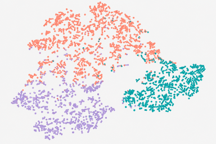
\includegraphics[width=0.45\linewidth]{figure/ACM_clusters.png}
    \caption{t-SNE visualization of learned ACM paper embeddings. Each point represents one paper, and color denotes its class.}
    \label{fig:clustering-acm}
\end{figure}

\begin{figure}[htbp]
    \centering
    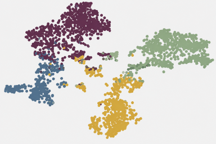
\includegraphics[width=0.45\linewidth]{figure/DBLP_clusters.png}
    \caption{t-SNE visualization of learned DBLP author embeddings. Each point represents one author, and color denotes its research area.}
    \label{fig:clustering-dblp}
\end{figure}

\begin{table}[htbp]
  \centering
  \caption{Additional clustering-quality diagnostics on DBLP and ACM,
  reported as mean $\pm$ standard deviation over five runs. Best mean
  values are bold.}
  \label{tab:clustering-diagnostic}
  \scriptsize
  \setlength{\tabcolsep}{2.5pt}
  \resizebox{\columnwidth}{!}{%
  \begin{tabular}{llcccc}
    \toprule
    & & \multicolumn{2}{c}{DBLP} & \multicolumn{2}{c}{ACM} \\
    \cmidrule(lr){3-4}
    \cmidrule(lr){5-6}
    \textbf{Group} & \textbf{Model}
    & NMI & ARI
    & NMI & ARI \\
    \midrule

    Hom./hom.
    & GAT
    & $71.50 \pm 0.36$
    & $77.26 \pm 0.48$
    & $57.22 \pm 0.19$
    & $60.47 \pm 0.31$ \\
    \midrule

    \multirow{2}{*}{Hom./het.}
    & NSD
    & $80.21 \pm 0.62$
    & $84.04 \pm 0.43$
    & $62.56 \pm 0.37$
    & $65.02 \pm 0.28$ \\

    & CSNN
    & $81.72 \pm 0.39$
    & $84.25 \pm 0.55$
    & $69.28 \pm 0.45$
    & $71.10 \pm 0.34$ \\
    \midrule

    \multirow{2}{*}{Het./hom.}
    & HAN
    & $79.12 \pm 0.47$
    & $84.76 \pm 0.58$
    & $60.63 \pm 0.22$
    & $64.28 \pm 0.41$ \\

    & PSHGCN
    & $80.38 \pm 0.52$
    & $82.65 \pm 0.36$
    & $71.89 \pm 0.49$
    & $74.31 \pm 0.57$ \\
    \midrule

    \multirow{2}{*}{Het./het.}
    & Hetero$^2$Net
    & $80.54 \pm 0.33$
    & $84.98 \pm 0.46$
    & $70.14 \pm 0.40$
    & $73.42 \pm 0.51$ \\

    & LatGRL
    & $81.36 \pm 0.56$
    & $86.07 \pm 0.38$
    & $72.52 \pm 0.61$
    & $76.75 \pm 0.44$ \\
    \midrule

    Ours
    & \textbf{\method{}}
    & $\mathbf{82.41 \pm 0.35}$
    & $\mathbf{86.52 \pm 0.42}$
    & $\mathbf{75.78 \pm 0.37}$
    & $\mathbf{78.29 \pm 0.31}$ \\
    \bottomrule
  \end{tabular}
  }
\end{table}
\section{Visualization of Node Embedding Separability During Training}
\label{sec:diffusion-process-analysis}

We further inspected the training dynamics of \method{} on the controlled four-class
\texttt{FakeHeteroDataset} from PyTorch Geometric \cite{FeyPyG2019,FeyPyG2025}. The model was trained with the default
synthetic-data settings, and the visualization includes only labeled nodes. We recorded the node
embeddings every five epochs. As shown in Figure~\ref{fig:fakehetero-diffusion-process}, nodes from
different classes are strongly interleaved at the beginning of training. As training proceeds, the
projected embeddings of nodes in the same class form increasingly compact and separated regions. This
observation suggests that training \method{} produces more class-separable node representations on
this controlled dataset.

\begin{figure}[htbp]
   \centering
   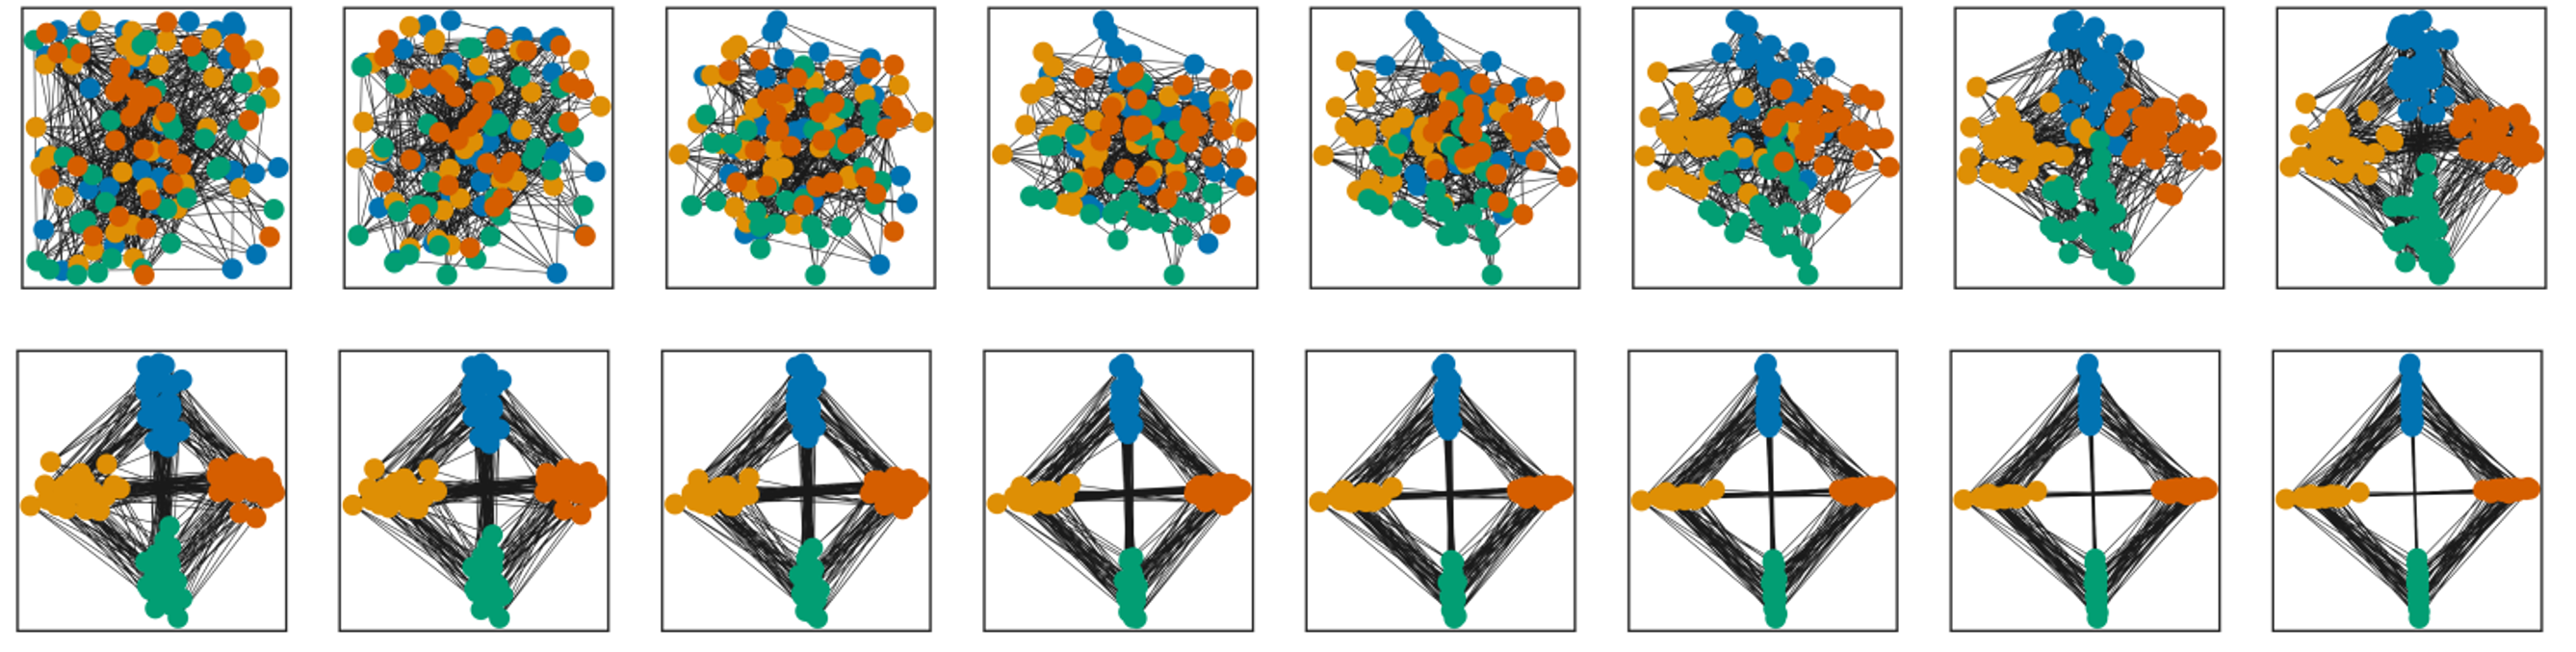
\includegraphics[width=\linewidth]{figure/fakehetero_diffusion_process.png}
   \caption{Qualitative visualization of node embedding dynamics during training on
the four-class \texttt{FakeHeteroDataset}.}
  \label{fig:fakehetero-diffusion-process}
\end{figure}


\section{Computational Efficiency}

To characterize the computational cost, we analyze the \method{} model, the
\ampss{} component, and \sheafcovpool{} readout.

Let \(N=|V|\) and \(M=|E|\) denote the numbers of nodes and observed directed
edges. Let \(N_{\mathrm{inst}}\) be the number of retained concrete path instances,
\[
I_{\mathrm{bnd}}=\sum_{f\in\mathcal{I}_{\mathrm{ret}}}(\ell_f+1)
\]
the number of boundary incidences, including one closure \(1\)-cell per
instance, and \(\widetilde M=M+N_{\mathrm{inst}}\) the size of the extended edge domain.
We use \(d\) for the stalk dimension and \(K\) for the number of diffusion
steps.

\paragraph{\ampss{}.}
Stage I runs once before training. Let \(C_\Sigma\) be the number of viable
schemas, \(S_{\max}\) the selection limit, \(N_p\) the number of probe examples,
\(B\) the feature width per schema, \(C_y\) the number of classes, and \(R_{\mathrm{sel}}\)
the number of probe iterations. Greedy selection evaluates
\(O(C_\Sigma S_{\max})\) subsets whose feature width grows to \(S_{\max}B\), giving
\[
O(R_{\mathrm{sel}}N_pBC_yC_\Sigma S_{\max}^2)
\]
probe time. Label propagation and schema/path enumeration additionally cost
\(O(K_{\mathrm{LP}}(M+N)C_y+Q_{\mathrm{type}}+Q_{\mathrm{samp}})\), where
\(K_{\mathrm{LP}}\) is the number of label-propagation iterations and the \(Q\) terms
count the visited typed and concrete path prefixes. Sparse coverage and
schema features require
\[
O(C_\Sigma L_{\max}+N_pS_{\max}B+N_{\mathrm{cov}}+I_{\mathrm{bnd}})
\]
storage, where \(L_{\max}\) is the maximum schema length and \(N_{\mathrm{cov}}\) is the
number of stored coverage entries. Stage II adds
\(O(N_{\mathrm{inst}}(h_f+d_r)h_\beta)\) instance-weighting time, where \(h_f\) is the
ordered-path latent width and \(h_\beta\) is the weighting-network width. The positive weights
do not prune operator tensors.

\paragraph{\method{}.}
To construct the scaled-orthogonal restriction maps, we use the Fast
Householder Product parameterization~\cite{mathiasen2020fasth}. Node-to-edge
maps are learned only for the \(M\) observed edges, whereas closure and
edge-to-face maps are obtained by path transport. Their dense
\(d\times d\) matrix operations require \(O((M+I_{\mathrm{bnd}})d^3)\) construction time.
The resulting maps are cached across diffusion steps, requiring
\(O((\widetilde M+I_{\mathrm{bnd}})d^2)\) space. Thus, map construction is cubic in the
stalk dimension, while memory grows quadratically.
Each matrix-free diffusion step applies the node-mediated and face-induced
components of the edge operator in
\[
O\!\left((\widetilde M+I_{\mathrm{bnd}})d^2+(N+\widetilde M)d\right)
\]
time. Hence, when the MLP widths and \(d_r\) scale with \(d\), the backbone
costs
\[
O\!\left(
Nd_{\mathrm{in}}d+(M+I_{\mathrm{bnd}})d^3
+K\bigl[(\widetilde M+I_{\mathrm{bnd}})d^2+(N+\widetilde M)d\bigr]
\right)
\]
time and
\[
O\!\left((\widetilde M+I_{\mathrm{bnd}})d^2+(N+\widetilde M+I_{\mathrm{bnd}})d\right)
\]
inference space. For fixed \(d\) and \(K\), both costs are linear in the
graph size and retained boundary incidences; no dense Laplacian is formed.

\paragraph{\sheafcovpool{}.}
With three node/edge views, projected dimension \(d_p\), pooling width \(h_p\),
\(N_{\mathrm{graph}}\) graphs, and \(C_{\mathrm{cls}}\) classes, the readout costs
\[
O\!\left(
\widetilde M d^2
+(N+\widetilde M)(d+h_pd_p+d_p^2)
+N_{\mathrm{graph}}(h_pd_p^2+h_pC_{\mathrm{cls}})
\right)
\]
time and
\[
O\!\left((N+\widetilde M)(d+d_p^2)+N_{\mathrm{graph}}d_p^2\right)
\]
space. The \(\widetilde M d^2\) term transports extended-edge states into
their endpoint stalks. With fixed dimensions, \sheafcovpool{} is linear in
the extended graph size and constructs neither a dense node-to-node
covariance matrix nor a coarsened graph.

Table~\ref{tab:efficiency} reports the measured runtime, parameter count, and memory usage on the
ACM node-classification task.

\begin{table}[htbp]
  \centering
  \caption{Efficiency comparison on ACM. Best values are bold. HetSheaf's code is unavailable, so we use the results reported for the HetSheaf ensemble model in the original paper.}
  \label{tab:efficiency}
  \scriptsize
  \begin{tabular}{lccc}
    \toprule
    \textbf{Model} & Runtime (s) & Parameters & Memory (MB) \\
    \midrule
    HAN & 28.9 & 2.2M & 1{,}780 \\
    HGT & 1{,}025.8 & 7.2M & 6{,}120 \\
    NSD & 47.6 & \textbf{155K} & \textbf{980} \\
    HetSheaf & 55.7 & 174K & - \\
    \midrule
    \textbf{\method{}} & 72.1 & 517K & 1120 \\
    \bottomrule
  \end{tabular}
\end{table}

Table~\ref{tab:efficiency} shows that \method{} requires more parameters, more memory, and has a higher runtime than other models including HetSheaf, the closest heterogeneous sheaf baseline. This is because \method{} retains path-supported \(2D\)-cells and performs sheaf-Hodge diffusion on both node and edge cochains, which increases the computational cost. However, \method{} achieves better performance than all baselines, as shown in Table~\ref{tab:node-cls}, Table~\ref{tab:link-pred}, and Table~\ref{tab:graph-cls}. This suggests that the additional computational cost of \method{} is justified by its superior performance.

\end{document}
